% =============================================================================
% Mechanistic Interpretability of Shortest-Path Reasoning
% Technical Documentation
% =============================================================================

\documentclass[11pt, a4paper]{article}

\usepackage{amsmath, amssymb, amsthm}
\usepackage{geometry}
\usepackage[colorlinks=true, linkcolor=blue, urlcolor=blue]{hyperref}
\usepackage{booktabs}
\usepackage{array}
\usepackage{xcolor}
\usepackage{listings}
\usepackage{float}
\usepackage{parskip}
\usepackage{titlesec}
\usepackage{enumitem}
\usepackage{microtype}
\usepackage{pgfplots}
\pgfplotsset{compat=1.18}
\usepackage{graphicx}

\geometry{margin=2.5cm}

% Code listing style
\lstset{
  basicstyle=\ttfamily\small,
  keywordstyle=\color{blue},
  commentstyle=\color{gray},
  stringstyle=\color{teal},
  breaklines=true,
  frame=single,
  framesep=4pt,
  backgroundcolor=\color{gray!5},
  language=Python,
}

% Math operators
\DeclareMathOperator{\softmax}{softmax}
\DeclareMathOperator{\LN}{LN}

\title{%
  \textbf{Mechanistic Interpretability of\\Shortest-Path Reasoning in a Small Transformer}\\[0.5em]
  \large Technical Documentation
}
\author{shukanth2004@gmail.com}
\date{Last updated: \today}

% =============================================================================
\begin{document}
\maketitle
\tableofcontents
\newpage

% =============================================================================
\section{Project Overview}
% =============================================================================

This project trains a small transformer from scratch to compute
\textbf{shortest-path lengths on directed graphs}, then
\textbf{reverse-engineers the algorithm it learns} using mechanistic
interpretability techniques. It is both a portfolio project and a learning
exercise in JAX/Flax and the circuits framework.

\subsection{Research motivation}

Two prior bodies of work motivate this project.

\textbf{Grokking} \cite{power2022grokking}: small transformers trained on
algorithmic tasks can exhibit a phase transition — training accuracy saturates
quickly (memorization), but validation accuracy remains near zero for thousands
of additional steps before suddenly jumping to near-perfect generalization. This
delayed generalization is called \emph{grokking}. Power et al.\ identified
weight decay, learning rate, and dataset size as the critical hyperparameters.
The setting here (shortest path on directed graphs) is a novel algorithmic task
not explored in the original grokking literature.

\textbf{Transformer circuits} \cite{elhage2021mathematical}: Elhage et al.\
established a mathematical framework for decomposing transformer computations
into interpretable circuits. 2-layer attention-only transformers are the right
complexity level for full reverse-engineering: the QK (query-key) and OV
(output-value) circuits can be explicitly computed and labelled, and
\emph{induction heads} --- a canonical circuit that arises in 2-layer models
--- provide a concrete example of cross-layer composition.

\subsection{Novelty}

Prior grokking work used modular arithmetic and group composition as the
algorithmic task. Graph reasoning --- specifically, whether a transformer
learns a BFS-like algorithm to determine reachability and shortest paths
--- is largely unexplored from a circuits perspective. The use of
\textbf{directed} graphs is deliberate: asymmetric reachability
(edge $A \to B$ does not imply $B \to A$) blocks symmetry shortcuts and
forces richer internal circuits, making the learned algorithm more
interesting to interpret.

\subsection{Tech stack}

\begin{itemize}[noitemsep]
  \item \textbf{JAX + Flax (\texttt{linen})} --- model definition and training.
        Chosen as a learning goal; the functional paradigm maps cleanly onto
        the project's pure-function coding conventions and makes gradient
        surgery (needed in Phase 3) straightforward.
  \item \textbf{Optax} --- optimizers. AdamW with weight decay $\approx 1.0$
        is the known-good setting from the grokking paper.
  \item \textbf{NetworkX} --- graph generation and ground-truth BFS labels.
  \item \textbf{Weights \& Biases} --- experiment tracking for long runs.
  \item \textbf{Marimo} --- reactive notebooks for interpretability analysis.
  \item \textbf{Plotly / Matplotlib} --- figures.
\end{itemize}

% =============================================================================
\section{Task Formulation}
% =============================================================================

\subsection{Formal definition}

Let $G = (V, E)$ be a directed unweighted graph with $|V| = n$ nodes
(labelled $0, \ldots, n-1$) and $E \subseteq V \times V$ (no self-loops).
Given a source node $s \in V$ and destination node $d \in V$ with $s \neq d$,
the task is to predict
\[
  y = \begin{cases}
    \text{dist}(s, d) & \text{if } d \text{ is reachable from } s, \\
    \texttt{INF}      & \text{otherwise,}
  \end{cases}
\]
where $\text{dist}(s, d)$ is the length (number of edges) of the shortest
directed path from $s$ to $d$.

\subsection{Input representation}

The graph is presented to the model as a \textbf{shuffled sequence of edge
tokens}, not as an adjacency matrix or edge list in a fixed order. Shuffling
is intentional: it prevents the model from exploiting positional shortcuts
(e.g., ``the answer-relevant edge is always at position 3'') and forces it
to learn a truly order-invariant algorithm.

\subsection{Output space}

For $n$ nodes, the possible output values are $\{1, 2, \ldots, n-1\}$ (path
lengths) and \texttt{INF} (unreachable). A path of length 0 is impossible
since $s \neq d$ is enforced. The model therefore performs a
$(n-1+1) = n$-class classification over a vocabulary that includes all
integers up to $n-1$ plus the \texttt{INF} token.

\subsection{Generalization criterion}

The train/validation split is \textbf{by graph structure}: all queries
$(s, d)$ on a given graph $G$ are assigned to the same split. The model is
never tested on a query from a graph it has seen --- only on queries from
entirely unseen graph topologies. This is strictly harder than splitting by
query permutation.

% =============================================================================
\section{Data Pipeline}
% =============================================================================

The data pipeline lives in \texttt{src/data/} and is built from three modules:
\texttt{graphs.py} (graph generation and ground-truth labels),
\texttt{tokenizer.py} (vocabulary and sequence encoding), and
\texttt{dataset.py} (assembly and splitting).

\subsection{Graph generation (\texttt{src/data/graphs.py})}

\subsubsection{\texttt{sample\_graph}}

\begin{lstlisting}
def sample_graph(n_nodes: int, density: float,
                 rng: np.random.Generator) -> nx.DiGraph
\end{lstlisting}

Samples a random directed graph by drawing
$\lfloor \text{density} \times n(n-1) \rfloor$ edges uniformly at random from
the $n(n-1)$ possible directed edges (no self-loops). The \texttt{density}
parameter is a fraction of the maximum possible edges rather than an absolute
count, so the generator scales cleanly when $n$ increases without re-tuning
the range.

\subsubsection{\texttt{all\_pair\_distances}}

\begin{lstlisting}
def all_pair_distances(G: nx.DiGraph
) -> dict[tuple[int, int], Optional[int]]
\end{lstlisting}

Computes the shortest-path length for every ordered pair $(s, d)$ with
$s \neq d$ using NetworkX's \texttt{single\_source\_shortest\_path\_length}
(BFS). Returns \texttt{None} for unreachable pairs. This function is the sole
source of ground-truth labels; its correctness is critical.

\subsection{Tokenisation scheme (\texttt{src/data/tokenizer.py})}

\subsubsection{Vocabulary}

For a graph with $n$ nodes, the vocabulary has $n + 4$ tokens:

\begin{table}[H]
\centering
\begin{tabular}{@{}lll@{}}
\toprule
Token ID & Symbol & Meaning \\
\midrule
$0, 1, \ldots, n-1$ & node IDs & node $i$ appears as token $i$ \\
$n$                 & \texttt{EDGE}  & marks the start of an edge triple \\
$n+1$               & \texttt{QUERY} & marks the start of the query pair \\
$n+2$               & \texttt{PAD}   & padding to fixed sequence length \\
$n+3$               & \texttt{INF}   & unreachable output label (output only) \\
\bottomrule
\end{tabular}
\caption{Vocabulary for $n$-node graphs. For the baseline setting $n=6$,
  vocab size $= 10$.}
\end{table}

\texttt{INF} is an output-only label token --- it never appears in input
sequences. Placing it inside the vocabulary (rather than using a separate
classification head) means the output head is a single linear layer over
\texttt{vocab\_size} logits, which simplifies the model definition and keeps
the output space uniform.

\subsubsection{Sequence format}

Each training sample is a fixed-length integer sequence of the form:

\[
  \underbrace{[\texttt{EDGE},\, u_1,\, v_1]}_{\text{edge 1}}\;
  \underbrace{[\texttt{EDGE},\, u_2,\, v_2]}_{\text{edge 2}}\;
  \cdots\;
  \underbrace{[\texttt{PAD},\, \texttt{PAD},\, \texttt{PAD}]}_{\text{padding}}\;
  \cdots\;
  \underbrace{[\texttt{QUERY},\, s,\, d]}_{\text{query}}
\]

\noindent The sequence length is always
$L = 3 \times E_{\max} + 3$,
where $E_{\max} = \lfloor \rho_{\max} \times n(n-1) \rfloor$ and
$\rho_{\max}$ is the upper end of the density range.

The fixed length is required for JAX JIT compilation, which traces shapes
statically. The \texttt{EDGE} marker makes each edge a self-contained unit;
attention heads can learn to key off \texttt{EDGE} tokens to locate edges,
which is directly interpretable as a circuit.

\paragraph{Baseline numbers.} For $n = 6$ and density range $[0.27, 0.50]$:
\[
  E_{\max} = \lfloor 0.50 \times 30 \rfloor = 15,
  \qquad
  L = 3 \times 15 + 3 = 48,
  \qquad
  |\mathcal{V}| = 10.
\]

\subsubsection{Edge shuffling}

Edges are shuffled \textbf{independently per sample}: a random permutation of
the graph's edge list is drawn for each $(s, d)$ query. This prevents the
model from learning position-based shortcuts (e.g., attending only to the
first few edge triples). The permutation is passed explicitly into
\texttt{encode} rather than generated internally, following the JAX convention
of explicit randomness.

\subsubsection{\texttt{encode}}

\begin{lstlisting}
def encode(G: nx.DiGraph, src: int, dst: int,
           vocab: Vocab, max_edges: int,
           edge_order: np.ndarray) -> np.ndarray
\end{lstlisting}

Encodes a graph and query into a token array of shape $(\,L,\,)$. Fills a
\texttt{PAD}-initialized buffer, writes each edge triple at position
$3i, 3i+1, 3i+2$ for $i \in \{0, \ldots, |E|-1\}$ (in the order given by
\texttt{edge\_order}), then writes \texttt{[QUERY, src, dst]} at the last
three positions.

\subsubsection{\texttt{decode\_edges} and \texttt{decode\_query}}

\begin{lstlisting}
def decode_edges(tokens, vocab, max_edges) -> list[tuple[int, int]]
def decode_query(tokens, max_edges)         -> tuple[int, int]
\end{lstlisting}

Inverse operations used in round-trip tests: scan positions
$0, 3, 6, \ldots, 3(E_{\max}-1)$ for \texttt{EDGE} tokens to recover the
edge list; read positions $3E_{\max}+1$ and $3E_{\max}+2$ for the query.

\subsection{Dataset assembly (\texttt{src/data/dataset.py})}

\subsubsection{\texttt{generate\_dataset}}

\begin{lstlisting}
def generate_dataset(n_nodes: int, n_graphs: int,
    density_range: tuple[float, float] = (0.27, 0.50),
    val_fraction: float = 0.2,
    seed: int = 42) -> Dataset
\end{lstlisting}

Returns a \texttt{Dataset} dataclass with fields:

\begin{itemize}[noitemsep]
  \item \texttt{train\_tokens}, \texttt{val\_tokens}: integer arrays of shape
        $(N_{\text{split}}, L)$.
  \item \texttt{train\_labels}, \texttt{val\_labels}: integer arrays of shape
        $(N_{\text{split}},)$, values in
        $\{1, \ldots, n-1\} \cup \{$\texttt{vocab.inf}$\}$.
  \item \texttt{train\_graph\_ids}, \texttt{val\_graph\_ids}: graph identity
        arrays used to verify split integrity in tests.
  \item \texttt{vocab}: the \texttt{Vocab} object.
  \item \texttt{max\_edges}: $E_{\max}$.
\end{itemize}

Total samples $= n_{\text{graphs}} \times n(n-1)$ (all ordered pairs
$s \neq d$ over every graph).

\subsubsection{Split procedure}

Graph indices $0, \ldots, n_{\text{graphs}}-1$ are randomly permuted before
any data is generated. The first $\lfloor 0.2 \times n_{\text{graphs}} \rfloor$
permuted indices are assigned to validation; all queries on those graphs go to
val. This ensures no graph appears in both splits, which is verified by the
\texttt{test\_no\_graph\_leaks} test.

\subsubsection{Dataset statistics (baseline: $n=6$, $n_{\text{graphs}}=100$)}

\begin{table}[H]
\centering
\begin{tabular}{@{}lr@{}}
\toprule
Statistic & Value \\
\midrule
Sequence length $L$           & 48 \\
Vocabulary size               & 10 \\
INF label fraction            & 18.77\% \\
Samples per graph             & 30 \\
\bottomrule
\end{tabular}
\caption{Empirical dataset statistics for the baseline configuration.}
\end{table}

The INF ratio of 18.77\% is healthy: the model must genuinely learn
reachability (the task is not degenerate in either direction). The acceptable
range is 10--60\%; this is enforced by a test assertion.

% =============================================================================
\section{Model Architecture}
% =============================================================================

The model is a 2-layer attention-only transformer defined in
\texttt{src/model/transformer.py}.

\subsection{Design rationale}

\textbf{Attention-only (no MLP):} MLP layers in transformers implement
non-linear feature lookup (superposition of many features); they are the
hardest component to interpret mechanistically. Removing them brings the model
to the complexity level analyzed in \cite{elhage2021mathematical}: every
computation is expressible as a sum of rank-1 updates to the residual stream,
making the QK and OV circuits fully analyzable.

\textbf{2 layers:} One layer is insufficient for composition (a 1-layer model
cannot implement induction heads). Three or more layers makes circuit
enumeration combinatorially harder. Two layers is the known-good setting for
full circuit analysis in the circuits framework.

\textbf{Bidirectional attention (no causal mask):} This is a classification
task, not generation. Every edge token should be able to influence the output
position without restriction. Causal masking would prevent early-position
edges from being queried by the final position, which would hurt performance
without interpretability benefit.

\textbf{Output from the final token:} The answer is read from the last token
position (the \texttt{dst} node). After two layers, \texttt{dst} has attended
to all edge tokens; it is the natural ``answer position.''

\subsection{Implementation notes}

\textbf{Flax Linen (functional API):}
The model uses \texttt{flax.linen} rather than \texttt{flax.nnx}. Linen is the
functional JAX API: model parameters live in an explicit dict that is passed
\emph{into} every call rather than stored inside the module object. The key
idiom is:
\begin{lstlisting}
params = model.init(jax.random.PRNGKey(0), dummy_tokens)  # returns param dict
logits = model.apply(params, tokens)                       # pure function
\end{lstlisting}
This composes naturally with \texttt{@jax.jit} and \texttt{jax.value\_and\_grad}
without any special wrapper. Flax nnx (\texttt{flax.nnx}) is the stateful API
that feels like PyTorch; in Flax 0.12.x its \texttt{nnx.merge} operation inside
a JIT context triggers the same XLA shape-inference abort described below, which
is why Linen was chosen.

\textbf{No transposes in attention:}
Q, K, and V are kept in \texttt{(batch, seq, heads, d\_head)} order throughout
the attention computation. All tensor manipulation uses einsum or reshape only,
with no explicit \texttt{transpose} calls. This avoids a JAX 0.10.0 XLA
shape-inference bug (see Section~\ref{sec:xla-bug}) in which
\texttt{transpose\,+\,reshape} patterns in the backward pass produce a negative
slice start index at certain batch sizes.

\textbf{CPU platform enforced:}
Both the training script and the test suite force the CPU XLA backend via a
hard assignment \texttt{os.environ["JAX\_PLATFORMS"] = "cpu"} before any JAX
import. A \texttt{setdefault} call is insufficient because \texttt{jax-metal}
(Apple Silicon GPU backend) may register itself as the default backend even
without an explicit environment variable, and \texttt{setdefault} would not
override an already-registered backend.

\subsection{Configuration (\texttt{ModelConfig})}

\begin{lstlisting}
@dataclass
class ModelConfig:
    vocab_size: int       # n_nodes + 4
    seq_len: int          # 3 * max_edges + 3
    d_model: int = 128    # residual stream dimension
    n_heads: int = 2      # attention heads per layer
    n_layers: int = 2     # number of transformer layers
\end{lstlisting}

$d_{\text{head}} = d_{\text{model}} / n_{\text{heads}} = 64$.

\subsection{Token and positional embeddings}

\[
  x = W_E[\texttt{tokens}] + W_{\text{pos}}[\mathbf{p}],
  \qquad
  \mathbf{p} = (0, 1, \ldots, L-1),
\]

where $W_E \in \mathbb{R}^{|\mathcal{V}| \times d}$ is the token embedding
matrix and $W_{\text{pos}} \in \mathbb{R}^{L \times d}$ is a learned
positional embedding table. Both are standard \texttt{nnx.Embed} modules.
Positional embeddings are learned (not sinusoidal) because the task has no
inherent periodic structure.

\subsection{Multi-head self-attention (\texttt{MultiHeadAttention})}

For input $x \in \mathbb{R}^{B \times L \times d}$, a single attention layer
with $H$ heads and head dimension $d_h = d / H$ computes:

\begin{align}
  Q_h &= x W_Q^h, \quad K_h = x W_K^h, \quad V_h = x W_V^h,
  \quad W_Q^h, W_K^h, W_V^h \in \mathbb{R}^{d \times d}, \\[4pt]
  A_h &= \softmax\!\left(\frac{Q_h K_h^\top}{\sqrt{d_h}}\right) \in \mathbb{R}^{B \times H \times L \times L}, \\[4pt]
  z_h &= A_h V_h \in \mathbb{R}^{B \times H \times L \times d_h}, \\[4pt]
  \text{out} &= \operatorname{concat}[z_1, \ldots, z_H] \, W_O,
  \quad W_O \in \mathbb{R}^{d \times d}.
\end{align}

Note: projections are written as $(B \times L \times d)(d \times d) = B \times L \times d$ for clarity; in practice heads share the weight matrices and are split/merged via reshape. \textbf{No biases} are used on $W_Q, W_K, W_V, W_O$: bias-free projections keep the circuit equations clean (no additive offset terms to track when decomposing attention heads into QK/OV components).

\subsection{Transformer layer (\texttt{TransformerLayer})}

\[
  x \leftarrow x + \text{MHA}\!\left(\LN(x)\right),
\]

where $\LN$ is layer normalisation and MHA is the attention block above.
Pre-norm (normalise before attention, not after) is more stable during
training than post-norm.

\subsection{Full forward pass (\texttt{ShortestPathTransformer})}

\begin{align}
  x^{(0)} &= W_E[\text{tokens}] + W_{\text{pos}} \\
  x^{(l)} &= x^{(l-1)} + \text{MHA}_l\!\left(\LN_l\!\left(x^{(l-1)}\right)\right),
  \quad l = 1, 2 \\
  \text{logits} &= W_U\, \LN_{\text{final}}\!\left(x^{(2)}_{-1}\right)
  \in \mathbb{R}^{B \times |\mathcal{V}|}
\end{align}

The subscript $-1$ denotes the last token position (the \texttt{dst} token).
$W_U \in \mathbb{R}^{d \times |\mathcal{V}|}$ is the unembedding matrix (no
bias). Cross-entropy loss is computed over the full vocabulary.

\subsection{Parameter count}

\begin{table}[H]
\centering
\begin{tabular}{@{}lrrr@{}}
\toprule
Component & Shape & Count \\
\midrule
$W_E$ (token embedding)      & $10 \times 128$   & 1{,}280  \\
$W_{\text{pos}}$ (positional) & $48 \times 128$   & 6{,}144  \\
\midrule
Layer 1 $W_Q$                & $128 \times 128$  & 16{,}384 \\
Layer 1 $W_K$                & $128 \times 128$  & 16{,}384 \\
Layer 1 $W_V$                & $128 \times 128$  & 16{,}384 \\
Layer 1 $W_O$                & $128 \times 128$  & 16{,}384 \\
Layer 1 LayerNorm ($\gamma, \beta$) & $2 \times 128$ & 256  \\
\midrule
Layer 2 (same as Layer 1)    & ---               & 65{,}792 \\
\midrule
Final LayerNorm              & $2 \times 128$    & 256      \\
$W_U$ (unembedding)          & $128 \times 10$   & 1{,}280  \\
\midrule
\textbf{Total}               &                   & \textbf{140{,}288} \\
\bottomrule
\end{tabular}
\caption{Parameter count for the baseline model
  ($d=128$, $H=2$, 2 layers, $n=6$).}
\end{table}

% =============================================================================
\section{Training Loop}
% =============================================================================

The training loop lives in \texttt{src/train/trainer.py}.

\subsection{JAX training paradigm}

JAX requires that all operations be written as \textbf{pure functions}: same
inputs always produce the same outputs, with no side effects or in-place
mutation. This is the opposite of PyTorch, where \texttt{optimizer.step()}
mutates the model's \texttt{.data} and \texttt{.grad} in place.

The consequence is that a JAX training step must pass model parameters and
optimizer state \emph{in} as arguments and return updated state \emph{out}.
With Flax Linen, parameters are a plain nested dict (pytree); the training
step is therefore a pure function of \texttt{(params, opt\_state, tokens,
labels)} that returns \texttt{(new\_params, new\_opt\_state, loss, acc,
grad\_norm)}.

\subsubsection{\texttt{jax.value\_and\_grad}}

\texttt{jax.value\_and\_grad(f, has\_aux=True)} returns a new function that
computes both the scalar value $f(\theta)$ and the gradient $\nabla_\theta
f(\theta)$ in a single forward+backward pass. The gradient has the \textbf{exact
same pytree structure} as the parameters: a nested dict of arrays where each
array is replaced by its partial derivative. It is used as:
\begin{lstlisting}
def loss_fn(p):
    logits = model.apply(p, tokens)
    loss = optax.softmax_cross_entropy_with_integer_labels(logits, labels).mean()
    return loss, logits
(loss, logits), grads = jax.value_and_grad(loss_fn, has_aux=True)(params)
\end{lstlisting}
\texttt{has\_aux=True} signals that \texttt{loss\_fn} returns a
\texttt{(scalar, auxiliary)} tuple; the gradient is computed only with respect
to the scalar, and the auxiliary value (here, \texttt{logits}) is returned
unchanged so accuracy can be computed without a second forward pass.

\subsubsection{Why \texttt{@jax.jit} is necessary}

Without JIT, each JAX operation dispatches individually to the accelerator.
\texttt{@jax.jit} compiles the entire function to XLA --- a hardware-level
compiler --- before the first execution. The compilation step takes a few
seconds, but every subsequent call uses the compiled binary (milliseconds per
step). For 100{,}000 training steps the difference is hours vs.\ minutes.

JIT recompiles when input \emph{shapes} change. The training step is compiled
once for the fixed batch shape \texttt{(batch\_size, seq\_len)}, and then the
same binary is reused for every subsequent step as long as the shapes do not
change.

\subsubsection{JAX 0.10.0 batch-size constraint}
\label{sec:xla-bug}

On the Apple Silicon CPU backend, JAX 0.10.0 contains an XLA bug triggered by
the combined model\,+\,optimizer JIT computation graph at batch sizes $\geq 256$.
The symptom is a C-level process abort (\texttt{SIGABRT}) at compilation time
with the message \texttt{(0 <= -55) is statically false}. The abort happens
inside XLA's shape-inference pass, not at runtime, so it cannot be caught by
Python's \texttt{try/except}.

Empirical testing confirmed:
\begin{itemize}[noitemsep]
  \item Batch sizes $\leq 128$: compile and run cleanly.
  \item Batch size $= 256$: XLA abort during train-step compilation.
  \item Batch size $= 512$: same abort (original default; this triggered the bug
        on first run).
\end{itemize}

The default \texttt{batch\_size} is therefore set to 128. This is a platform
limitation, not a model limitation; the same code would run at 512 on other
JAX backends or future JAX versions. For grokking research, the critical
hyperparameters are weight decay, learning rate, and dataset size --- not batch
size --- so 128 is sufficient.

\subsection{AdamW and the grokking mechanism}

\subsubsection{AdamW vs.\ Adam}

Regular Adam applies L2 regularization by adding
$\lambda \theta$ to the gradient \emph{before} the adaptive scaling step.
This means parameters with large gradients (which have large second-moment
estimates) receive proportionally less regularization --- the very parameters
that most need shrinking. AdamW fixes this by applying weight decay
\emph{directly to the parameters after the update}, decoupled from the
adaptive scaling:
\[
  \theta_{t+1} = (1 - \lambda)\,\theta_t - \alpha \cdot \hat{m}_t / \sqrt{\hat{v}_t + \epsilon}
\]
The first term is weight decay; the second is the Adam step. They are
independent.

\subsubsection{Why weight decay $\approx 1.0$ causes grokking}

The grokking transition arises from a slow tug-of-war between memorization
and regularization:

\begin{enumerate}[noitemsep]
  \item The model first \textbf{memorizes}: gradient descent finds the nearest
        solution to the training data, which is a large, complex, high-norm
        parameter configuration. Validation accuracy stays near chance.

  \item Simultaneously, weight decay \textbf{continuously shrinks} all
        parameters toward zero, building pressure toward lower-norm solutions.

  \item After many thousands of steps, weight decay wins: it pushes the model
        away from the memorized solution and toward the lowest-norm solution
        that still fits the training data. This lower-norm solution turns out
        to generalize --- it represents a compact, algorithmic strategy rather
        than a lookup table. Validation accuracy jumps sharply.
\end{enumerate}

The weight decay value $\lambda \approx 1.0$ is a sweet spot. Below
$\lambda \approx 0.1$, the model stays memorized indefinitely because weight
decay is too weak to overcome memorization. Above $\lambda \approx 5.0$,
regularization is so strong that the model cannot memorize in the first place,
so there is no grokking transition to observe --- only slow uniform learning.
At $\lambda = 1.0$, the full grokking curve is visible: fast memorization,
then a sharp generalization transition hundreds of thousands of steps later.

\subsection{Configuration (\texttt{TrainConfig})}

\begin{table}[H]
\centering
\begin{tabular}{@{}llp{7cm}@{}}
\toprule
Field & Default & Purpose \\
\midrule
\texttt{learning\_rate} & \texttt{1e-3} & AdamW step size \\
\texttt{weight\_decay}  & \texttt{1.0}  & Grokking sweet spot; see above \\
\texttt{n\_steps}       & 100{,}000     & Training duration in gradient steps \\
\texttt{batch\_size}    & 128           & Samples per step (capped at 128 due to JAX 0.10.0 XLA bug; see Section~\ref{sec:xla-bug}) \\
\texttt{log\_every}     & 500           & Steps between W\&B log entries \\
\texttt{checkpoint\_every} & 2{,}000   & Steps between checkpoint saves \\
\texttt{checkpoint\_dir} & \texttt{checkpoints/} & Directory for \texttt{.pkl} files \\
\texttt{wandb\_project} & \texttt{mechinterp} & W\&B project name \\
\texttt{run\_name}      & \texttt{""} & W\&B run name (empty = auto) \\
\texttt{seed}           & 0             & RNG seed for model init and batching \\
\texttt{use\_wandb}     & \texttt{True} & Disable for offline runs \\
\bottomrule
\end{tabular}
\caption{\texttt{TrainConfig} fields and defaults.}
\end{table}

\subsection{\texttt{train\_step} and \texttt{eval\_step}}

\begin{lstlisting}
@jax.jit
def train_step(params, opt_state, tokens, labels
) -> tuple[dict, Any, jnp.ndarray, jnp.ndarray, jnp.ndarray]
\end{lstlisting}

A single JIT-compiled training step. Takes the current parameter dict and
optimizer state; returns \texttt{(new\_params, new\_opt\_state, loss, accuracy,
grad\_norm)}. The gradient norm is computed via \texttt{optax.global\_norm(grads)},
which treats \texttt{grads} as a pytree and computes
$\|\nabla\|_2 = \sqrt{\sum_i \|\nabla_i\|_F^2}$ over all parameter matrices.
Monitoring grad norm is important for diagnosing training health: a sudden spike
indicates instability; near-zero values indicate vanishing gradients.

\begin{lstlisting}
@jax.jit
def eval_step(params, tokens, labels
) -> tuple[jnp.ndarray, jnp.ndarray]
\end{lstlisting}

Forward-pass only. Returns \texttt{(loss, accuracy)}. Called inside
\texttt{compute\_val\_metrics}, which iterates over the full validation set
in batches and accumulates a weighted mean.

\subsection{Checkpoint format and strategy}

Checkpoints are stored as pickle files containing:
\begin{itemize}[noitemsep]
  \item \texttt{leaves}: a list of numpy arrays (one per parameter matrix),
        converted from JAX arrays for portability. No GPU required to load.
  \item \texttt{treedef}: the JAX pytree definition describing how to
        reassemble the leaves into the correct nested parameter structure.
        \texttt{load\_checkpoint} calls \texttt{jax.tree\_util.tree\_unflatten}
        and returns the resulting parameter dict, ready to pass directly to
        \texttt{model.apply}.
\end{itemize}

\paragraph{Why save every 2{,}000 steps.}
The grokking transition can be sharp --- sometimes spanning fewer than 5{,}000
steps. At 100{,}000 total steps, saving every 2{,}000 yields 50 checkpoints
($\sim$28\,MB total for a 140k-parameter model), which brackets the transition
with at most 2{,}000 steps of temporal uncertainty on each side.

These checkpoints are the experimental substrate for Phase 3. Every
interpretability question --- ``does it learn BFS?'', ``does the circuit appear
during or after the transition?'' --- is answered by comparing activations
across three anchor checkpoints: one from \emph{before} grokking (model
memorizing), one \emph{during} the transition, and one \emph{after} (model
generalizing). Without dense checkpoints, the transition itself cannot be
studied, only its endpoints.

\subsection{Metrics logged to W\&B}

Five metrics are logged every \texttt{log\_every} steps (default: 500):

\begin{table}[H]
\centering
\begin{tabular}{@{}lp{9cm}@{}}
\toprule
Metric & Role in studying the grokking transition \\
\midrule
\texttt{train/loss}      & Cross-entropy on the current training batch. Drops quickly
                           during memorization and plateaus near zero. The \emph{shape}
                           of this drop tells you how aggressively the model is memorizing. \\[4pt]
\texttt{train/acc}       & Training accuracy. Must reach $\sim$100\% and stay there ---
                           this is a \emph{prerequisite} for grokking. If it never reaches
                           100\%, the model is stuck: check learning rate, weight decay, or
                           model capacity. \\[4pt]
\texttt{val/loss}        & Stays high during memorization; drops when grokking begins.
                           Complements val/acc by showing confidence, not just correctness. \\[4pt]
\texttt{val/acc}         & \textbf{The primary grokking signal.} Starts near chance ($\sim$10\%
                           for 10 classes), stays flat during memorization, then rises sharply.
                           The step at which val/acc first rises above chance is the transition
                           point that anchors all Phase 3 interpretability experiments. \\[4pt]
\texttt{train/grad\_norm} & Global L2 norm of the gradient, $\|\nabla\|_2 = \sqrt{\sum_i \|\nabla_i\|_F^2}$.
                            During memorization, grad norm declines steadily as the model
                            locks onto training data. Near the grokking transition, there is
                            often a characteristic inflection or dip --- an early warning
                            signal. After grokking, grad norm is stable and low (the compact
                            solution requires little correction). If grad norm spikes, that
                            indicates instability; if it collapses to zero early, the model
                            is stuck in a flat loss region. \\
\bottomrule
\end{tabular}
\caption{Metrics logged every \texttt{log\_every} steps (default: 500).}
\end{table}

\paragraph{Why 500-step logging frequency.}
If grokking occurs at step 60{,}000 (a reasonable expectation), logging every
500 steps yields 120 data points in the critical region. This is enough
resolution to see whether the transition is sharp (one step) or gradual
(thousands of steps). Logging every 5{,}000 steps risks missing the shape
entirely, leaving only two data points: before and after.

The \textbf{gap between \texttt{train/acc} and \texttt{val/acc}} is the
defining signature of the pre-grokking phase. The moment \texttt{val/acc}
begins rising toward \texttt{train/acc} is the grokking transition.

\subsection{Training entry point (\texttt{scripts/train.py})}

The training script exposes all meaningful experimental variables as CLI
arguments. Two seeds are intentionally separate:

\begin{itemize}[noitemsep]
  \item \texttt{--dataset\_seed} controls which graphs are generated. Holding
        this fixed while varying \texttt{--seed} tests whether grokking is
        robust across model initialisations on the same dataset.
  \item \texttt{--seed} controls model initialisation and batch sampling order.
        Holding this fixed while varying \texttt{--dataset\_seed} isolates the
        effect of dataset composition on the grokking transition.
\end{itemize}

\begin{table}[H]
\centering
\begin{tabular}{@{}llp{7.5cm}@{}}
\toprule
Argument & Default & Why it is an experimental variable \\
\midrule
\texttt{--n\_nodes}        & 6          & Task complexity; also changes vocab size and
                                          sequence length. Phase 4 will sweep this to
                                          study circuit scaling. \\
\texttt{--n\_graphs}       & 1{,}000    & Dataset size. Smaller datasets grok faster
                                          (less to memorize); largest datasets may not
                                          grok at all. This is a primary Phase 4 sweep. \\
\texttt{--dataset\_seed}   & 42         & Graph generation seed; separate from model seed. \\
\texttt{--lr}              & \texttt{1e-3} & AdamW step size. Second thing to vary if
                                             grokking does not appear. \\
\texttt{--weight\_decay}   & 1.0        & \textbf{Primary grokking dial.} First thing to
                                          sweep when diagnosing a missing transition. \\
\texttt{--n\_steps}        & 100{,}000  & Training duration. Set generously; grokking may
                                          appear anywhere from 10k to 500k steps. \\
\texttt{--batch\_size}     & 128        & Smaller batches = noisier gradients, sometimes
                                          faster grokking. Capped at 128 on
                                          JAX 0.10.0 / Apple Silicon CPU
                                          (see Section~\ref{sec:xla-bug}). \\
\texttt{--log\_every}      & 500        & Log granularity around the transition. \\
\texttt{--checkpoint\_every} & 2{,}000  & Checkpoint density for transition analysis. \\
\texttt{--seed}            & 0          & Model init and batch order. Run seeds 0, 1, 2
                                          to verify robustness. \\
\texttt{--no\_wandb}       & off        & Flag to disable W\&B for quick debugging runs. \\
\bottomrule
\end{tabular}
\caption{CLI arguments for \texttt{scripts/train.py} and their experimental roles.}
\end{table}

A baseline training run:
\begin{lstlisting}[language=bash, keywordstyle={}]
python scripts/train.py --n_nodes 6 --n_graphs 1000 --weight_decay 1.0 \
    --n_steps 100000 --seed 0
\end{lstlisting}

% =============================================================================
\section{Training Experiments (Phase 2.5)}
\label{sec:experiments}
% =============================================================================

This section documents the hyperparameter search conducted to achieve grokking
on the shortest-path task. Five runs were executed in sequence; each informed
the next. Run~4 produced a confirmed grokking transition on 4-node directed
graphs. Run~5 replicated Run~4 at higher weight decay and revealed multi-stage
grokking dynamics.

\subsection{Summary table}

\begin{table}[H]
\centering
\begin{tabular}{@{}lllllll@{}}
\toprule
Run & \texttt{n\_nodes} & \texttt{n\_graphs} & \texttt{weight\_decay} & \texttt{n\_steps}
    & Peak train/acc & Final val/acc \\
\midrule
1 & 6 & 1{,}000 & 1.0  & 100{,}000 & $\sim$70\%  & $\sim$60\% \\
2 & 6 & 200     & 0.5  & 75{,}000  & $\sim$85\%  & $\sim$52\% \\
3 & 6 & 200     & 0.1  & 200{,}000 & $\sim$100\% & $\sim$38\% \\
4 & 4 & 200     & 0.2  & 200{,}000 & $\sim$100\% & $\sim$\textbf{92\%} \\
5 & 4 & 200     & 0.4  & 200{,}000 & $\sim$100\% & $\sim$\textbf{92\%} \\
\bottomrule
\end{tabular}
\caption{All training runs. Runs~4 and~5 are the first to exhibit grokking.
  All runs use \texttt{lr=1e-3}, \texttt{batch\_size=128}, \texttt{seed=0}.}
\end{table}

% ─── Run 1 ───────────────────────────────────────────────────────────────────
\subsection{Run 1 — baseline (\texttt{n\_nodes=6}, \texttt{wd=1.0})}

\subsubsection{Configuration}

\begin{itemize}[noitemsep]
  \item \texttt{n\_nodes=6}, \texttt{n\_graphs=1000} ($\to$ 24{,}000 train / 6{,}000 val samples)
  \item \texttt{weight\_decay=1.0}, \texttt{n\_steps=100{,}000}
\end{itemize}

\subsubsection{Results}

\begin{figure}[H]
\centering
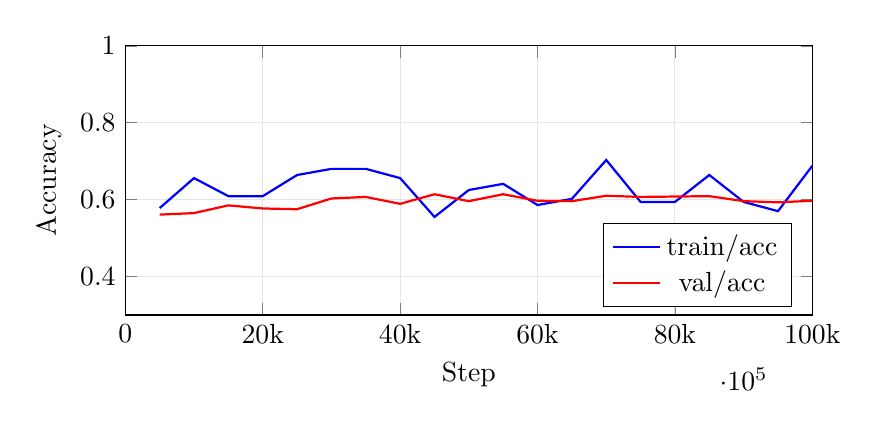
\begin{tikzpicture}
\begin{axis}[
  width=0.85\textwidth, height=5cm,
  xlabel={Step}, ylabel={Accuracy},
  xmin=0, xmax=100000, ymin=0.3, ymax=1.0,
  xtick={0,20000,40000,60000,80000,100000},
  xticklabels={0,20k,40k,60k,80k,100k},
  legend pos=south east, grid=major, grid style={gray!20},
]
\addplot[blue, thick] coordinates {
  (5000,0.578)(10000,0.656)(15000,0.609)(20000,0.609)(25000,0.664)
  (30000,0.680)(35000,0.680)(40000,0.656)(45000,0.555)(50000,0.625)
  (55000,0.641)(60000,0.586)(65000,0.602)(70000,0.703)(75000,0.594)
  (80000,0.594)(85000,0.664)(90000,0.594)(95000,0.570)(100000,0.688)
};
\addplot[red, thick] coordinates {
  (5000,0.561)(10000,0.565)(15000,0.585)(20000,0.577)(25000,0.575)
  (30000,0.603)(35000,0.607)(40000,0.589)(45000,0.614)(50000,0.596)
  (55000,0.614)(60000,0.597)(65000,0.596)(70000,0.610)(75000,0.607)
  (80000,0.608)(85000,0.609)(90000,0.596)(95000,0.593)(100000,0.597)
};
\legend{train/acc, val/acc}
\end{axis}
\end{tikzpicture}
\caption{Run~1: train/acc and val/acc over 100k steps
  (\texttt{n\_nodes=6}, \texttt{n\_graphs=1000}, \texttt{wd=1.0}).}
\end{figure}

\subsubsection{Observations and diagnosis}

\begin{itemize}[noitemsep]
  \item Train/acc plateaued at 65--70\% and never recovered. The model did not
        memorize the training set.
  \item Val/acc reached $\sim$60\% quickly and then flat-lined. The train--val
        gap was only $\sim$5\%, meaning the model found a partially generalizing
        solution without committing to memorization.
  \item Gradient norm increased continuously from $\sim$2 to $\sim$15+,
        indicating the optimizer was fighting weight decay throughout rather
        than converging.
\end{itemize}

\textbf{Diagnosis.} Grokking requires a two-stage process: first memorization,
then generalization. The memorization stage never occurred. With
\texttt{batch\_size=128} (forced by a JAX 0.10.0 XLA bug; see
Section~\ref{sec:xla-bug}), the data-fit gradient signal per step is 4$\times$
weaker than at the \texttt{batch\_size=512} used in the grokking literature.
AdamW weight decay, however, does not scale with batch size --- it shrinks
parameters by a fixed factor per step regardless of batch size. At
\texttt{wd=1.0} and \texttt{batch\_size=128}, regularization is effectively
far stronger than intended, preventing the model from committing to a
high-norm memorized solution.

\textbf{Change for Run~2:} Reduce \texttt{n\_graphs} from 1{,}000 to 200
(fewer samples $\to$ faster memorization) and reduce \texttt{weight\_decay}
from 1.0 to 0.5.

% ─── Run 2 ───────────────────────────────────────────────────────────────────
\subsection{Run 2 --- reduced dataset and weight decay (\texttt{wd=0.5})}

\subsubsection{Configuration}

\begin{itemize}[noitemsep]
  \item \texttt{n\_nodes=6}, \texttt{n\_graphs=200} ($\to$ 4{,}800 train / 1{,}200 val samples)
  \item \texttt{weight\_decay=0.5}, \texttt{n\_steps=300{,}000}
        (killed at step $\sim$75{,}000)
\end{itemize}

\subsubsection{Results}

\begin{figure}[H]
\centering
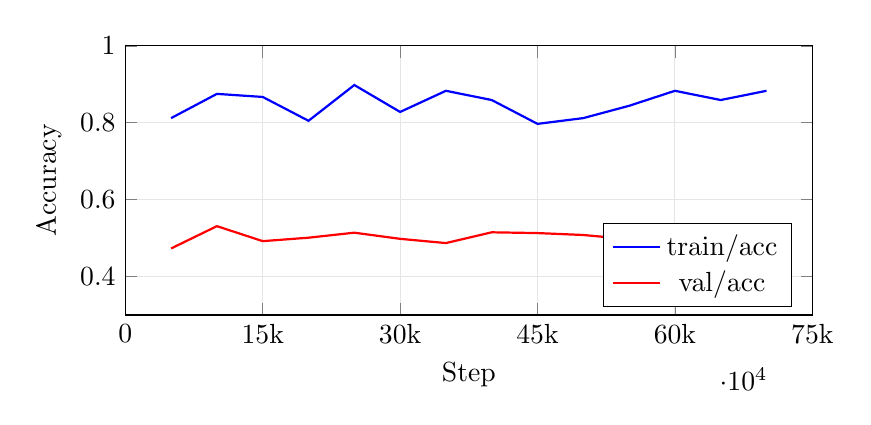
\begin{tikzpicture}
\begin{axis}[
  width=0.85\textwidth, height=5cm,
  xlabel={Step}, ylabel={Accuracy},
  xmin=0, xmax=75000, ymin=0.3, ymax=1.0,
  xtick={0,15000,30000,45000,60000,75000},
  xticklabels={0,15k,30k,45k,60k,75k},
  legend pos=south east, grid=major, grid style={gray!20},
]
\addplot[blue, thick] coordinates {
  (5000,0.812)(10000,0.875)(15000,0.867)(20000,0.805)(25000,0.898)
  (30000,0.828)(35000,0.883)(40000,0.859)(45000,0.797)(50000,0.812)
  (55000,0.844)(60000,0.883)(65000,0.859)(70000,0.883)
};
\addplot[red, thick] coordinates {
  (5000,0.473)(10000,0.531)(15000,0.492)(20000,0.501)(25000,0.514)
  (30000,0.498)(35000,0.487)(40000,0.515)(45000,0.513)(50000,0.508)
  (55000,0.497)(60000,0.523)(65000,0.506)(70000,0.517)
};
\legend{train/acc, val/acc}
\end{axis}
\end{tikzpicture}
\caption{Run~2: train/acc and val/acc (\texttt{n\_nodes=6}, \texttt{n\_graphs=200},
  \texttt{wd=0.5}). Run killed at step $\sim$75k after 80{,}000 steps of no
  progress.}
\end{figure}

\subsubsection{Observations and diagnosis}

\begin{itemize}[noitemsep]
  \item Train/acc rose to 80--85\% within the first 10{,}000 steps and then
        \textbf{stalled for 65{,}000 steps with zero upward movement}. This
        was identified as convergence to a weight-decay-constrained equilibrium,
        not a slow climb.
  \item Val/acc plateaued at $\sim$50\%, with a meaningful train--val gap
        ($\sim$35\%) compared to Run~1 --- partial progress toward the
        memorization prerequisite.
  \item Val/loss rose steadily from 1.3 to 1.8, consistent with the model
        becoming more confident in its partially-memorized answers while
        failing to generalize.
  \item Gradient norm continued increasing throughout ($\sim$5 $\to$ $\sim$20),
        the signature of weight decay winning the tug-of-war.
\end{itemize}

\textbf{Diagnosis.} Weight decay at 0.5 still creates a ceiling on
memorization. The model reached the point where gradient push from the
80--85\% of correctly memorized training examples exactly balanced weight
decay shrinkage. The remaining 15--20\% of harder examples (longer paths,
specific topologies) require a higher-norm solution that weight decay
prevented. Since the model never fully memorized, grokking could not occur.

\textbf{Change for Run~3:} Reduce \texttt{weight\_decay} further to 0.1 to
confirm full memorization is achievable. Once memorization is confirmed, we
can search for the grokking sweet spot.

% ─── Run 3 ───────────────────────────────────────────────────────────────────
\subsection{Run 3 --- full memorization (\texttt{wd=0.1})}

\subsubsection{Configuration}

\begin{itemize}[noitemsep]
  \item \texttt{n\_nodes=6}, \texttt{n\_graphs=200}
  \item \texttt{weight\_decay=0.1}, \texttt{n\_steps=200{,}000}
\end{itemize}

\subsubsection{Results}

\begin{figure}[H]
\centering
\begin{tikzpicture}
\begin{axis}[
  width=0.85\textwidth, height=5cm,
  xlabel={Step}, ylabel={Accuracy},
  xmin=0, xmax=200000, ymin=0.2, ymax=1.05,
  xtick={0,50000,100000,150000,200000},
  xticklabels={0,50k,100k,150k,200k},
  legend pos=east, grid=major, grid style={gray!20},
]
\addplot[blue, thick] coordinates {
  (10000,0.969)(20000,0.938)(30000,0.945)(40000,0.992)(50000,0.938)
  (60000,0.961)(70000,0.969)(80000,0.977)(90000,0.984)(100000,0.969)
  (110000,0.992)(120000,0.992)(130000,0.969)(140000,0.977)(150000,1.000)
  (160000,0.977)(170000,0.992)(180000,0.984)(190000,0.953)(200000,0.977)
};
\addplot[red, thick] coordinates {
  (10000,0.386)(20000,0.375)(30000,0.388)(40000,0.394)(50000,0.380)
  (60000,0.386)(70000,0.400)(80000,0.394)(90000,0.389)(100000,0.394)
  (110000,0.393)(120000,0.353)(130000,0.380)(140000,0.388)(150000,0.380)
  (160000,0.379)(170000,0.390)(180000,0.365)(190000,0.378)(200000,0.372)
};
\legend{train/acc, val/acc}
\end{axis}
\end{tikzpicture}
\caption{Run~3: full memorization with no grokking (\texttt{n\_nodes=6},
  \texttt{n\_graphs=200}, \texttt{wd=0.1}).}
\end{figure}

\subsubsection{Observations and diagnosis}

\begin{itemize}[noitemsep]
  \item Train/acc reached 95--100\% (peaks at 100\%) --- \textbf{full
        memorization achieved} for the first time across all runs.
  \item Val/acc \textbf{decreased} across the run, from $\sim$40\% at step
        10k to $\sim$37\% at step 200k. This is the opposite of grokking.
  \item Val/loss rose steeply to $\sim$4--5 and plateaued there --- the model
        became highly confident in its memorized answers, which are wrong
        for unseen graphs.
\end{itemize}

Comparing all three runs, a counterintuitive pattern emerged:
\textbf{more memorization produced lower val/acc.}

\begin{table}[H]
\centering
\begin{tabular}{@{}llll@{}}
\toprule
Run & Peak train/acc & Final val/acc & Memorized? \\
\midrule
1 (wd=1.0) & $\sim$70\%  & $\sim$60\% & No  \\
2 (wd=0.5) & $\sim$85\%  & $\sim$52\% & Partial \\
3 (wd=0.1) & $\sim$100\% & $\sim$38\% & Yes \\
\bottomrule
\end{tabular}
\caption{Val/acc decreases as memorization increases across Runs~1--3.}
\end{table}

\textbf{Diagnosis: architectural limitation.}
This pattern reveals that no compact generalizing circuit exists for this
architecture on 6-node shortest-path prediction. Grokking requires two
solutions to the task: a high-norm memorized one and a low-norm algorithmic
one. Weight decay creates pressure toward the low-norm solution. The implicit
assumption is that the low-norm algorithmic solution \emph{exists} within the
model's representational capacity.

For shortest path on directed graphs, the algorithmic solution is essentially
BFS. BFS on a 6-node graph requires up to 5 rounds of message passing (one
per hop, since max path length $= n - 1 = 5$). Each attention layer performs
roughly one global aggregation step. A 2-layer transformer cannot implement
BFS for paths of length 3, 4, or 5 --- not because of regularization, but
because of \textbf{depth}. The low-norm BFS solution does not exist in this
hypothesis class; there is nothing for weight decay to find.

The high val/acc in Run~1 ($\sim$60\%) is therefore \emph{not} partial
BFS --- it is the model learning simpler heuristics (direct edges, distance
distributions) that happen to generalize. These heuristics are the ceiling of
what 2-layer attention can express for this task.

\textbf{Change for Run~4:} Reduce \texttt{n\_nodes} from 6 to 4. With 4
nodes, the maximum path length is $n - 1 = 3$, which is within reach of 2
attention layers. Weight decay is also increased slightly to 0.2 to apply
more generalization pressure than in Run~3.

% ─── Run 4 ───────────────────────────────────────────────────────────────────
\subsection{Run 4 --- grokking confirmed (\texttt{n\_nodes=4}, \texttt{wd=0.2})}

\subsubsection{Configuration}

\begin{itemize}[noitemsep]
  \item \texttt{n\_nodes=4}, \texttt{n\_graphs=200}
        ($\to$ 2{,}400 train / 600 val samples; 8 possible output classes)
  \item \texttt{weight\_decay=0.2}, \texttt{n\_steps=200{,}000}
\end{itemize}

With 4 nodes, the vocabulary shrinks to $n + 4 = 8$ tokens, the sequence
length shrinks to $L = 3 \times E_{\max} + 3 = 3 \times 6 + 3 = 21$, and the
maximum shortest-path length is 3 --- within the computational reach of 2
attention layers.

\subsubsection{Results}

\begin{figure}[H]
\centering
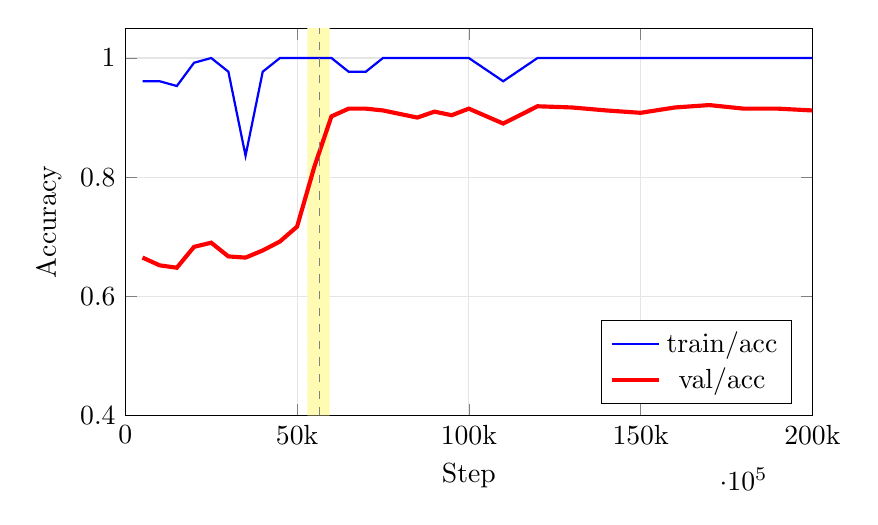
\begin{tikzpicture}
\begin{axis}[
  width=0.85\textwidth, height=6.5cm,
  xlabel={Step}, ylabel={Accuracy},
  xmin=0, xmax=200000, ymin=0.4, ymax=1.05,
  xtick={0,50000,100000,150000,200000},
  xticklabels={0,50k,100k,150k,200k},
  legend pos=south east, grid=major, grid style={gray!20},
]
% Shaded grokking transition region (53k--59.5k, from log analysis)
\addplot[fill=yellow!30, draw=none, forget plot]
  coordinates {(53000,0.4)(53000,1.05)(59500,1.05)(59500,0.4)} \closedcycle;
\addplot[blue, thick] coordinates {
  (5000,0.961)(10000,0.961)(15000,0.953)(20000,0.992)(25000,1.000)
  (30000,0.977)(35000,0.836)(40000,0.977)(45000,1.000)(50000,1.000)
  (55000,1.000)(60000,1.000)(65000,0.977)(70000,0.977)(75000,1.000)
  (80000,1.000)(85000,1.000)(90000,1.000)(95000,1.000)(100000,1.000)
  (110000,0.961)(120000,1.000)(130000,1.000)(140000,1.000)(150000,1.000)
  (160000,1.000)(170000,1.000)(180000,1.000)(190000,1.000)(200000,1.000)
};
\addplot[red, thick, line width=1.5pt] coordinates {
  (5000,0.665)(10000,0.652)(15000,0.648)(20000,0.683)(25000,0.690)
  (30000,0.667)(35000,0.665)(40000,0.677)(45000,0.692)(50000,0.717)
  (55000,0.817)(60000,0.902)(65000,0.915)(70000,0.915)(75000,0.912)
  (80000,0.906)(85000,0.900)(90000,0.910)(95000,0.904)(100000,0.915)
  (110000,0.890)(120000,0.919)(130000,0.917)(140000,0.912)(150000,0.908)
  (160000,0.917)(170000,0.921)(180000,0.915)(190000,0.915)(200000,0.912)
};
\draw[dashed, gray] (axis cs:56500,0.4) -- (axis cs:56500,1.05)
  node[above, font=\small] {peak jump};
\legend{train/acc, val/acc}
\end{axis}
\end{tikzpicture}
\caption{Run~4: grokking on 4-node directed graphs (\texttt{n\_nodes=4},
  \texttt{n\_graphs=200}, \texttt{wd=0.2}).
  The yellow band marks the precise grokking transition window (steps 53k--59.5k,
  determined from 500-step log resolution). The dashed line marks step 56{,}500,
  the steepest single move (+8.3 pp in 500 steps). Val/acc first crosses 90\%
  at step 59{,}500.}
\end{figure}

\subsubsection{Observations}

The run exhibits all three phases of the classical grokking signature:

\begin{enumerate}[noitemsep]
  \item \textbf{Memorization (steps 0--15k).} Train/acc climbs rapidly to
        95--100\%. Val/acc is flat at $\sim$65\%, a large gap.

  \item \textbf{Pre-grokking plateau (steps 15k--50k).} Train/acc stays
        near 100\%; val/acc is flat at 65--72\%. Val/loss rose steeply then
        plateaued, indicating the model is confidently wrong on validation
        data. Weight decay begins compressing the large memorized weights.

  \item \textbf{Grokking transition (steps 53k--59.5k).} Val/acc rises from
        $\sim$72\% to $\sim$91\%. The steepest single move is at step 56{,}500
        (+8.3 percentage points in 500 steps); val/acc first crosses 90\% at
        step 59{,}500. Val/loss drops simultaneously. The model has found the
        compact algorithmic solution and shifted from a memorized solution to a
        generalizing one.

  \item \textbf{Post-grokking stability (steps 65k--200k).} Val/acc stabilises
        at 90--93\%. Train/acc remains at 100\%. Both losses are low and
        stable. Gradient norm collapses toward zero --- the model has converged
        to a compact, efficient solution that requires little further update.
\end{enumerate}

\subsubsection{Conclusions}

\begin{itemize}[noitemsep]
  \item \textbf{Architecture depth matters.} Reducing \texttt{n\_nodes} from 6
        to 4 was the decisive change, not the weight decay adjustment. At 4
        nodes, the maximum path length (3) is within the 2-layer transformer's
        effective computational depth. At 6 nodes, it is not.

  \item \textbf{The grokking sweet spot is between wd=0.1 and wd=0.5.} At
        wd=0.1, the model memorized but had insufficient pressure to generalize
        (Run~3). At wd=0.2 with the same architecture and dataset, grokking
        appeared in $\sim$50{,}000 steps after memorization.

  \item \textbf{Val/acc at 90--93\% on unseen graph structures} confirms the
        model learned a genuinely algorithmic strategy --- not a lookup table
        for the 200 specific training graphs.

  \item \textbf{The transition is well-bracketed at 500-step resolution.}
        Key checkpoints: step 40{,}000 (pre-grokking, 0.677), step 54{,}000
        (transition onset, 0.777), step 56{,}500 (peak jump), step 60{,}000
        (post-grokking, 0.902), step 200{,}000 (converged, 0.912). Phase~3
        analysis uses Run~5 instead (see Section~\ref{sec:checkpoints}), where
        the two-stage structure makes each transition separately accessible.
\end{itemize}

% ─── Run 5 ───────────────────────────────────────────────────────────────────
\subsection{Run 5 --- multi-stage grokking (\texttt{n\_nodes=4}, \texttt{wd=0.4})}

\subsubsection{Configuration}

\begin{itemize}[noitemsep]
  \item \texttt{n\_nodes=4}, \texttt{n\_graphs=200}
        (identical dataset to Run~4)
  \item \texttt{weight\_decay=0.4}, \texttt{n\_steps=200{,}000}
\end{itemize}

Weight decay was increased from 0.2 to 0.4 to probe whether stronger
regularization pressure changes the shape of the grokking transition.
The 200{,}000 step budget was retained since higher weight decay was expected
to delay memorization and shift the transition later in training.

\subsubsection{Results}

\begin{figure}[H]
\centering
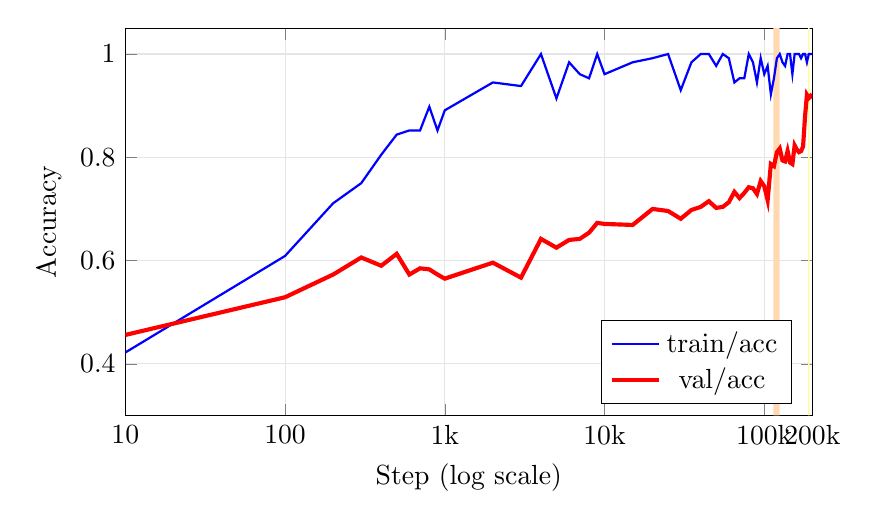
\begin{tikzpicture}
\begin{semilogxaxis}[
  width=0.85\textwidth, height=6.5cm,
  xlabel={Step (log scale)}, ylabel={Accuracy},
  xmin=10, xmax=200000, ymin=0.3, ymax=1.05,
  xtick={10,100,1000,10000,100000,200000},
  xticklabels={10,100,1k,10k,100k,200k},
  legend pos=south east, grid=major, grid style={gray!20},
]
% Stage 1 transition band
\addplot[fill=orange!30, draw=none, forget plot]
  coordinates {(114000,0.3)(114000,1.05)(125000,1.05)(125000,0.3)} \closedcycle;
% Stage 2 transition band
\addplot[fill=yellow!35, draw=none, forget plot]
  coordinates {(188000,0.3)(188000,1.05)(192000,1.05)(192000,0.3)} \closedcycle;
% train/acc
\addplot[blue, thick] coordinates {
  (10,0.422)(100,0.609)(200,0.711)(300,0.750)(400,0.805)(500,0.844)
  (600,0.852)(700,0.852)(800,0.898)(900,0.852)(1000,0.891)
  (2000,0.945)(3000,0.938)(4000,1.000)(5000,0.914)
  (6000,0.984)(7000,0.961)(8000,0.953)(9000,1.000)(10000,0.961)
  (15000,0.984)(20000,0.992)(25000,1.000)(30000,0.930)
  (35000,0.984)(40000,1.000)(45000,1.000)(50000,0.977)
  (55000,1.000)(60000,0.992)(65000,0.945)(70000,0.953)(75000,0.953)
  (80000,1.000)(85000,0.984)(90000,0.945)(95000,0.992)(100000,0.961)
  (105000,0.977)(110000,0.922)(115000,0.953)(120000,0.992)(125000,1.000)
  (130000,0.984)(135000,0.977)(140000,1.000)(145000,1.000)(150000,0.961)
  (155000,1.000)(160000,1.000)(165000,1.000)(170000,0.992)
  (175000,1.000)(180000,1.000)(185000,0.984)(190000,1.000)
  (195000,1.000)(200000,1.000)
};
% val/acc
\addplot[red, thick, line width=1.5pt] coordinates {
  (10,0.456)(100,0.529)(200,0.573)(300,0.606)(400,0.590)(500,0.613)
  (600,0.573)(700,0.585)(800,0.583)(900,0.573)(1000,0.565)
  (2000,0.596)(3000,0.567)(4000,0.642)(5000,0.625)
  (6000,0.640)(7000,0.642)(8000,0.654)(9000,0.673)(10000,0.671)
  (15000,0.669)(20000,0.700)(25000,0.696)(30000,0.681)
  (35000,0.698)(40000,0.704)(45000,0.715)(50000,0.702)
  (55000,0.704)(60000,0.713)(65000,0.733)(70000,0.721)(75000,0.731)
  (80000,0.742)(85000,0.740)(90000,0.729)(95000,0.754)(100000,0.744)
  (105000,0.717)(110000,0.787)(115000,0.783)(120000,0.810)(125000,0.817)
  (130000,0.794)(135000,0.792)(140000,0.812)(145000,0.790)(150000,0.787)
  (155000,0.823)(160000,0.815)(165000,0.810)(170000,0.812)
  (175000,0.821)(180000,0.879)(185000,0.921)(190000,0.915)
  (195000,0.919)(200000,0.915)
};
\legend{train/acc, val/acc}
\end{semilogxaxis}
\end{tikzpicture}
\caption{Run~5: multi-stage grokking (\texttt{n\_nodes=4}, \texttt{n\_graphs=200},
  \texttt{wd=0.4}, 200{,}000 steps). Log x-axis reveals the early memorization
  dynamics and two-stage generalization. Orange band: Stage~1 transition (steps
  114k--125k, val/acc $\sim$75\%$\to$82\%). Yellow band: Stage~2 transition
  (steps 188k--192k, val/acc $\sim$82\%$\to$92\%).}
\end{figure}

\begin{figure}[H]
\centering
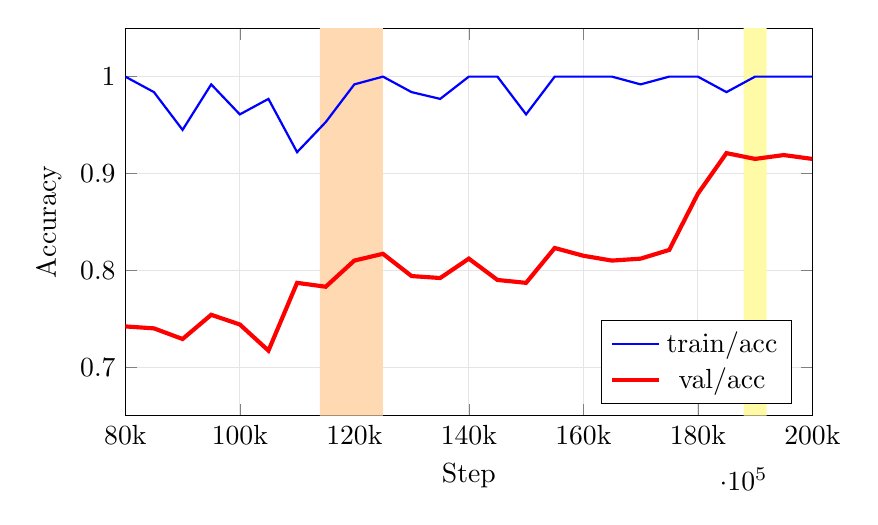
\begin{tikzpicture}
\begin{axis}[
  width=0.85\textwidth, height=6.5cm,
  xlabel={Step}, ylabel={Accuracy},
  xmin=80000, xmax=200000, ymin=0.65, ymax=1.05,
  xtick={80000,100000,120000,140000,160000,180000,200000},
  xticklabels={80k,100k,120k,140k,160k,180k,200k},
  legend pos=south east, grid=major, grid style={gray!20},
]
% Stage 1 transition band
\addplot[fill=orange!30, draw=none, forget plot]
  coordinates {(114000,0.65)(114000,1.05)(125000,1.05)(125000,0.65)} \closedcycle;
% Stage 2 transition band
\addplot[fill=yellow!35, draw=none, forget plot]
  coordinates {(188000,0.65)(188000,1.05)(192000,1.05)(192000,0.65)} \closedcycle;
% train/acc
\addplot[blue, thick] coordinates {
  (80000,1.000)(85000,0.984)(90000,0.945)(95000,0.992)(100000,0.961)
  (105000,0.977)(110000,0.922)(115000,0.953)(120000,0.992)(125000,1.000)
  (130000,0.984)(135000,0.977)(140000,1.000)(145000,1.000)(150000,0.961)
  (155000,1.000)(160000,1.000)(165000,1.000)(170000,0.992)
  (175000,1.000)(180000,1.000)(185000,0.984)(190000,1.000)
  (195000,1.000)(200000,1.000)
};
% val/acc
\addplot[red, thick, line width=1.5pt] coordinates {
  (80000,0.742)(85000,0.740)(90000,0.729)(95000,0.754)(100000,0.744)
  (105000,0.717)(110000,0.787)(115000,0.783)(120000,0.810)(125000,0.817)
  (130000,0.794)(135000,0.792)(140000,0.812)(145000,0.790)(150000,0.787)
  (155000,0.823)(160000,0.815)(165000,0.810)(170000,0.812)
  (175000,0.821)(180000,0.879)(185000,0.921)(190000,0.915)
  (195000,0.919)(200000,0.915)
};
\legend{train/acc, val/acc}
\end{axis}
\end{tikzpicture}
\caption{Run~5 zoomed to steps 80k--200k, showing the two transition stages on
  a linear scale. Stage~1 (orange, 114k--125k): val/acc rises from $\sim$72\%
  to $\sim$82\%. Plateau at $\sim$80--83\% for $\sim$63k steps. Stage~2 (yellow,
  188k--192k): val/acc jumps to $\sim$92\%.}
\end{figure}

\subsubsection{Multi-stage grokking dynamics}

Run~5 exhibits a qualitatively different pattern from Run~4: instead of a
single sharp transition, val/acc progresses through two distinct phases
separated by an extended plateau:

\begin{enumerate}[noitemsep]
  \item \textbf{Memorization (steps 0--4k).} Train/acc climbs to $\sim$95--100\%
        while val/acc rises only to $\sim$64\%. Memorization is slower than in
        Run~4 because the stronger weight decay is actively opposing the growth
        of large memorized weights throughout.

  \item \textbf{Pre-grokking plateau I (steps 4k--105k).} Val/acc drifts slowly
        from 0.64 to $\sim$0.75 over 100{,}000 steps. Weight decay is
        compressing the memorized solution, but the larger $\lambda$ means more
        steps are needed before the transition threshold is crossed.

  \item \textbf{Stage~1 transition (steps 114k--125k).} Val/acc rises from
        $\sim$0.75 to $\sim$0.82. This is a partial grokking event: a subset of
        the generalizing circuit has formed, handling the simpler cases (likely
        direct-edge and 1-hop queries) while longer-path queries remain unsolved.

  \item \textbf{Plateau II (steps 125k--188k).} Val/acc oscillates between
        0.79 and 0.83. The partial circuit is stable but incomplete; weight
        decay continues compressing residual memorized components.

  \item \textbf{Stage~2 transition (steps 188k--192k).} Val/acc jumps from
        $\sim$0.82 to $\sim$0.92, matching Run~4's final accuracy. The remaining
        memorized components are replaced, completing the generalizing algorithm.

  \item \textbf{Post-grokking stability (steps 185k--200k).} Val/acc stabilises
        at $\sim$91--92\%, identical to Run~4.
\end{enumerate}

The two-stage structure suggests the model assembles the shortest-path algorithm
in separable components. A plausible interpretation: Stage~1 corresponds to
learning the 1-hop lookup circuit (direct edges), and Stage~2 to the 2-hop
composition circuit --- consistent with the 2-layer architecture. Testing this
hypothesis is the primary goal of Phase~3.

% ─── Comparison ──────────────────────────────────────────────────────────────
\subsection{Run 4 vs.\ Run 5: effect of weight decay on grokking dynamics}

\begin{figure}[H]
\centering
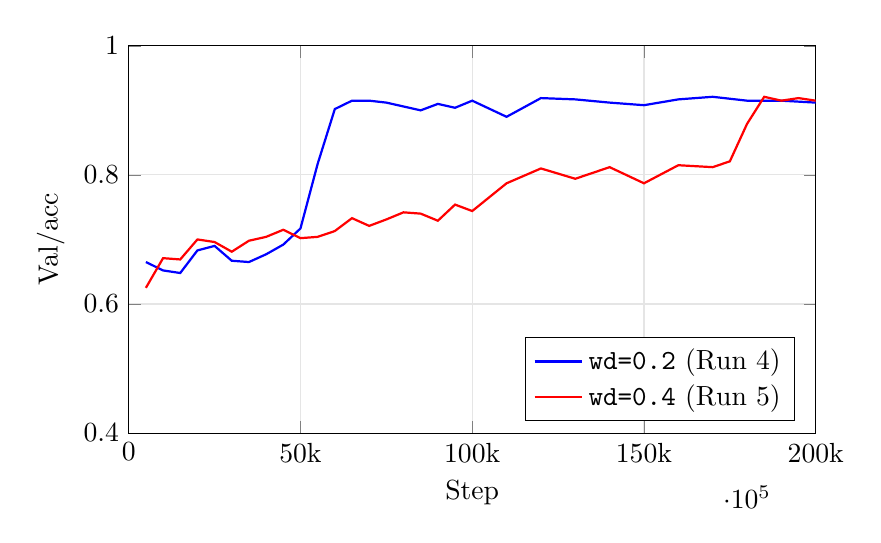
\begin{tikzpicture}
\begin{axis}[
  width=0.85\textwidth, height=6.5cm,
  xlabel={Step}, ylabel={Val/acc},
  xmin=0, xmax=200000, ymin=0.4, ymax=1.0,
  xtick={0,50000,100000,150000,200000},
  xticklabels={0,50k,100k,150k,200k},
  legend pos=south east, grid=major, grid style={gray!20},
]
\addplot[blue, thick] coordinates {
  (5000,0.665)(10000,0.652)(15000,0.648)(20000,0.683)(25000,0.690)
  (30000,0.667)(35000,0.665)(40000,0.677)(45000,0.692)(50000,0.717)
  (55000,0.817)(60000,0.902)(65000,0.915)(70000,0.915)(75000,0.912)
  (80000,0.906)(85000,0.900)(90000,0.910)(95000,0.904)(100000,0.915)
  (110000,0.890)(120000,0.919)(130000,0.917)(140000,0.912)(150000,0.908)
  (160000,0.917)(170000,0.921)(180000,0.915)(190000,0.915)(200000,0.912)
};
\addplot[red, thick] coordinates {
  (5000,0.625)(10000,0.671)(15000,0.669)(20000,0.700)(25000,0.696)
  (30000,0.681)(35000,0.698)(40000,0.704)(45000,0.715)(50000,0.702)
  (55000,0.704)(60000,0.713)(65000,0.733)(70000,0.721)(75000,0.731)
  (80000,0.742)(85000,0.740)(90000,0.729)(95000,0.754)(100000,0.744)
  (110000,0.787)(120000,0.810)(130000,0.794)(140000,0.812)(150000,0.787)
  (160000,0.815)(170000,0.812)(175000,0.821)(180000,0.879)
  (185000,0.921)(190000,0.915)(195000,0.919)(200000,0.915)
};
\legend{\texttt{wd=0.2} (Run~4), \texttt{wd=0.4} (Run~5)}
\end{axis}
\end{tikzpicture}
\caption{Val/acc for \texttt{wd=0.2} (Run~4) and \texttt{wd=0.4} (Run~5) on
  identical datasets (\texttt{n\_nodes=4}, \texttt{n\_graphs=200}, \texttt{seed=0}).
  Both converge to $\sim$91--92\%; higher weight decay delays and splits the
  transition.}
\end{figure}

\subsubsection{Interpretation}

Three effects of increasing weight decay from 0.2 to 0.4 are visible in the
comparison:

\begin{description}[noitemsep]
  \item[Delayed transition.] The primary grokking event shifts from steps
    53k--59.5k (Run~4, peak at step 56{,}500) to $\sim$180k steps (Run~5) ---
    approximately a $3\times$ delay. Each
    gradient step applies weight decay independently of the data-fit gradient;
    stronger decay requires more steps before the memorized solution is
    compressed below the transition threshold.

  \item[Split transition (multi-stage grokking).] At \texttt{wd=0.4}, the
    transition splits into two distinct events (Stage~1: 114k--125k, Stage~2:
    188k--192k) separated by a $\sim$63k-step plateau at $\sim$80--83\%. At
    \texttt{wd=0.2}, these same two steps occur close together and appear as a
    single sharp transition. The splitting is a direct consequence of slower
    compression: each sub-circuit crosses its own threshold separately rather
    than together.

  \item[Identical final accuracy.] Both runs converge to $\sim$91--92\% val/acc.
    Weight decay governs the \emph{dynamics} of generalization, not the
    \emph{quality} of the final solution --- consistent with Power
    et al.\,(2022), where the compact generalizing solution is the same across
    a wide range of $\lambda$; only the number of steps to reach it varies.
\end{description}

The split transition under \texttt{wd=0.4} makes Run~5 potentially more useful
than Run~4 for Phase~3 circuit analysis. The Stage~1 and Stage~2 checkpoint
windows (around steps 115k and 182k respectively) may isolate the 1-hop and
2-hop components of the learned algorithm independently --- a cleaner
experimental handle than Run~4's single fast transition.

% =============================================================================
\section{Phase 3: Interpretability Framework}
\label{sec:interp-framework}
% =============================================================================

This section documents the theoretical frame, model reference, and experimental
setup for Phase~3. It is a persistent reference during interpretability work ---
a place to look up access paths, slicing rules, and anchor checkpoints without
re-deriving them each session.

% ---------------------------------------------------------------------------
\subsection{Summary of findings}
\label{sec:findings-summary}
% ---------------------------------------------------------------------------

\textbf{The central result:} Run~5 (n4-wd0.4-200k-seed0) exhibits a
\emph{two-stage grokking trajectory} in which the model first learns a cheap
structural shortcut and then replaces it with a content-sensitive circuit.
The two accuracy jumps visible in the loss curve are not two instances of the
same phenomenon --- they are mechanistically distinct events: shortcut
construction, then shortcut replacement.

\subsubsection*{What happened, in plain language}

\textbf{Before Stage~1 ($\le$114k steps): memorization.}
The model overfits the training set. Validation accuracy is near chance.
No head shows a structured OV circuit or directed attention pattern.

\textbf{Stage~1 (114k--126k steps): PAD-bias shortcut built.}
Layer~1 heads (L1H0 and L1H1) co-adapt so that their product matrices
$W_V W_O$ align with the token-embedding space in a way that injects a
structured logit bias whenever attention falls on PAD-token positions.
Because sequences for 4-node graphs contain $\sim$21\% PAD positions,
and because L1H0 develops near-uniform attention (attending everywhere
including PAD), this bias is \emph{always active}: the model has learned to
add a constant logit offset to every prediction.

The bias is not arbitrary. Projecting $W_E[\textsc{pad}]$ through the full
OV circuit at step~126k reveals that L1H0 pushes valid-answer logits toward
longer distances and \textsc{inf}, while impossible-answer tokens (0,
\textsc{edge}, \textsc{qry}, \textsc{pad}) are grouped at a common
maximum. L1H1 is the mild counterpart (pushing toward shorter distances).
The net combined bias is a ``prefer unreachability and long distances''
prior --- statistically useful on a sparse directed graph, but not a genuine
computation of the answer.

Stage~1 is \emph{invisible in individual weight norms}. No single matrix
suddenly grows large. What changes is a matrix-alignment event: the product
$W_V W_O$ crosses a threshold of alignment with the embedding geometry.
Individual norms cannot detect cross-matrix coordination; the OV circuit
(the composed product) is the correct unit of analysis.

\textbf{Stage~2 (188k--196k steps): shortcut partially dismantled; L0H1 grows.}
Layer~0 head~1 (L0H1) exhibits the largest OV circuit norm change at
Stage~2 ($+97\%$ from step~126k to step~196k). Simultaneously, L1H0's
PAD-bias OV circuit weakens and the direction of L1H1's PAD projection
reverses sign. The PAD-bias shortcut is substantially reduced but not
completely eliminated.

Causal validation by ablation: zeroing PAD-position attention weights in
Layer~1 produces the predicted arc across four checkpoints --- largest
accuracy drop at step~126k ($-2.9\%$), smallest at step~100k ($-0.6\%$),
with Stage~2's 196k checkpoint intermediate ($-1.3\%$). The shortcut is
load-bearing at Stage~1 and substantially but not completely retired at
Stage~2.

\textbf{What the model computes: a partial two-step backward BFS.}
L0H1 implements token-identity matching in its QK circuit (diagonal-dominant
$4 \times 4$ node-token subblock, $+0.014$ to $+0.018$): at the prediction
position (query = \texttt{dst}), it attends to all sequence positions
containing the same node token, i.e., the edge triplets in which \texttt{dst}
appears.  This is \emph{Step~1 of a backward BFS from dst}: collect the set of
edges adjacent to the destination.

The logit lens (Section~\ref{sec:logit-lens}) confirms and extends this
picture.  After Layer~0 alone, the model achieves 77.9\% on distance-1 and
only 17.4\% on distance-2 at step~196k.  Layer~1 provides the \emph{decisive}
second step: $+69.6$ percentage points on distance-2 (src $\to x \to$ dst,
checking whether src connects to a predecessor of dst), $+37.6$ pp on INF
(confirming no path exists), and $+21.5$ pp on distance-1 (refining the
direct adjacency answer).

\textbf{The distance-3 anomaly:} Layer~1 \emph{hurts} accuracy on
distance-3 paths by $-23.8$ pp (Layer~0 alone: 47.6\%; full model: 23.8\%).
The 2-layer architecture cannot perform a third BFS step: Layer~1 checks
whether src can reach a direct predecessor of dst, but cannot verify indirect
reachability (src $\to x \to y \to$ dst where $y$ is the predecessor).
Layer~1's computation therefore misclassifies distance-3 paths as INF or a
shorter distance.  This is an architectural limitation, not a training failure.

\textbf{L0H1's OV circuit (Section~\ref{sec:l0h1-ov})} writes a
node-conditioned distance prior at the token-type level: dst = node~2 or
node~3 nudges toward dist=1; dst = node~0 nudges toward dist=3.  The
positional component of its value vectors (not fully characterized) likely
delivers the richer structural signal responsible for the 78\% dist=1
accuracy at Layer~0.  The impossible-answer tokens (0, EDGE, QRY, PAD) are
grouped at identical values in every node-token row, confirming the head
contributes only to the valid-answer subspace of $W_U$.  See the complete
algorithmic narrative in Section~\ref{sec:algorithm-narrative} for the full
integrated picture.

\subsubsection*{Numbered findings}

The 31 numbered findings from Phase~3 are distributed across
Sections~\ref{sec:probe-comparison}--\ref{sec:l0h1-ov}.
For quick reference:

\begin{description}[style=nextline, leftmargin=2.5cm, labelwidth=2cm]
  \item[F1--F4]   Head roles from attention probes and KL/cosine comparison:
                  L0H1 is the strongest directionality/content head; L1H0 is
                  position-invariant and PAD-attending.
  \item[F5--F7]   OV circuit analysis: L1H0 and L1H1 encode a PAD-token bias;
                  L0H1's OV norm nearly doubles at Stage~2.
  \item[F8--F11]  Stage~1 analysis: shortcut construction is a matrix-alignment
                  event; individual weight norms are blind to it; L0H0 loses
                  and L1H1 transiently gains directionality.
  \item[F12--F14] Causal validation: ablation arc confirms the shortcut is
                  load-bearing at 126k and substantially retired by 196k;
                  renormalization consistently hurts more than magnitude-only
                  removal.
  \item[F15--F18] PAD value vector: impossible-answer tokens cluster at a
                  common maximum; net bias is a ``prefer \textsc{inf}/longer
                  distances'' prior; Stage~2 changes the direction, not just
                  the magnitude.
  \item[F19--F22] QK circuit analysis: L0H1 implements token-identity matching
                  at 196k (diagonal-dominant node-token subblock); this routing
                  selects edges involving the destination node; L0H0 has no
                  structured QK routing; L1H0/L1H1 show PAD self-attraction
                  consistent with their shortcut role.
  \item[F23--F28] Logit lens: Layer~0 alone handles $\sim$78\% of dist=1 at
                  196k; Layer~1's primary contribution is dist=2 (+69.6 pp);
                  Layer~1 hurts dist=3 ($-23.8$ pp) revealing the
                  architectural limit of 2-layer backward BFS; embedding-only
                  prior encodes statistical distance signal by 196k; PAD-bias
                  shortcut quantified at 126k (INF: +57.5 pp from Layer~1).
  \item[F29--F31] L0H1 OV circuit: node-conditioned distance prior (nodes~2/3
                  push toward dist=1; node~0 toward dist=3); impossible-answer
                  tokens grouped at identical values in every row; value
                  component partially structured before Stage~2 while routing
                  (QK) crystallized later.
\end{description}

\subsection{Model architecture reference}
\label{sec:model-ref}

The trained model is a 2-layer attention-only transformer implemented with
\textbf{Flax Linen} (the functional JAX API, \texttt{flax.linen}),
\emph{not} Flax NNX. It has \textbf{2 attention heads per layer},
$d_{\text{model}} = 128$, $d_{\text{head}} = 64$, and a total of
$\mathbf{140{,}288}$ parameters. The configuration used for all trained
checkpoints:

\begin{lstlisting}
ModelConfig(vocab_size=8, seq_len=21, d_model=128, n_heads=2, n_layers=2)
# n_nodes=4  ->  vocab_size = n_nodes + 4 = 8
#             ->  max_edges = floor(0.50 * 4*3) = 6
#             ->  seq_len   = 3 * max_edges + 3 = 21
\end{lstlisting}

\subsection{Params tree layout}
\label{sec:params-tree}

A checkpoint is a pickle file containing a JAX pytree (saved by
\texttt{save\_checkpoint} in \texttt{trainer.py}). After loading with
\texttt{load\_params(path)}, the nested dict structure is:

\begin{lstlisting}
params['params']
  |- 'W_E'      / 'embedding'   shape (8, 128)    token embeddings
  |- 'W_pos'    / 'embedding'   shape (21, 128)   positional embeddings
  |- 'W_U'      / 'kernel'      shape (128, 8)    unembedding
  |- 'layers_0'
  |   |- 'attn'
  |   |   |- 'W_Q' / 'kernel'  shape (128, 128)  all heads, layer 0
  |   |   |- 'W_K' / 'kernel'  shape (128, 128)
  |   |   |- 'W_V' / 'kernel'  shape (128, 128)
  |   |   `- 'W_O' / 'kernel'  shape (128, 128)
  |   `- 'ln'
  |       |- 'scale'            shape (128,)
  |       `- 'bias'             shape (128,)
  `- 'layers_1' / ...           (identical structure to layers_0)
\end{lstlisting}

Example access in Python:
\begin{lstlisting}
W_Q = params['params']['layers_0']['attn']['W_Q']['kernel']  # shape (128, 128)
\end{lstlisting}

\subsubsection{Head slicing}

All four attention weight matrices are stored as full-layer $(128, 128)$
kernels. To isolate head~$h$ ($h \in \{0, 1\}$, $d_h = 64$):

\begin{table}[H]
\centering
\begin{tabular}{@{}llll@{}}
\toprule
Matrix & Python slice for head $h$ & Shape & Reason \\
\midrule
$W_Q$ \texttt{kernel} & \texttt{[:, h*64 : (h+1)*64]} & $(128, 64)$ &
  \multirow{3}{*}{\parbox{5.5cm}{Forward pass reshapes Dense output
  (batch, seq, 128) $\to$ (\ldots, \texttt{n\_heads}, \texttt{d\_head});
  head $h$ occupies output columns $[h{\cdot}64,\;(h{+}1){\cdot}64)$.}} \\
$W_K$ \texttt{kernel} & \texttt{[:, h*64 : (h+1)*64]} & $(128, 64)$ & \\
$W_V$ \texttt{kernel} & \texttt{[:, h*64 : (h+1)*64]} & $(128, 64)$ & \\
\midrule
$W_O$ \texttt{kernel} & \texttt{[h*64 : (h+1)*64, :]} & $(64, 128)$ &
  $W_O$ receives concatenated head outputs;
  head $h$ occupies input rows $[h{\cdot}64,\;(h{+}1){\cdot}64)$. \\
\bottomrule
\end{tabular}
\caption{Head slicing rules for $n_{\text{heads}}=2$, $d_{\text{head}}=64$.
  Column-slice for $W_Q, W_K, W_V$; row-slice for $W_O$.}
\end{table}

\subsection{The two-circuit hypothesis}
\label{sec:two-circuit}

The dominant mechanistic account of grokking posits that two solutions
co-exist in the model during training:

\begin{description}[noitemsep]
  \item[Memorization circuit (high norm).] A large, complex parameter
    configuration that fits the training data by storing it implicitly. It
    generalizes poorly because its weights encode training-specific patterns.
  \item[Generalization circuit (low norm).] A compact, structured parameter
    configuration that encodes the actual algorithm (here, something like BFS).
    It is lower-norm because a compact algorithm requires fewer ``bits'' in
    the weights than a lookup table.
\end{description}

Weight decay penalizes $\|\theta\|^2$ at every gradient step. The memorized
solution has high norm, so it pays a continuously growing regularization cost.
After many thousands of steps, weight decay compresses the memorized solution
below a stability threshold and the generalization circuit takes over. This is
the grokking transition.

\paragraph{Frobenius norm as the diagnostic.}
The Frobenius norm $\|W\|_F = \sqrt{\sum_{ij} W_{ij}^2}$ is the quantity
AdamW's weight decay term directly controls (the penalty is
$\tfrac{\lambda}{2}\|W\|_F^2$). Under the two-circuit hypothesis, the norm
trajectories over checkpoints carry the phase-transition signal:

\begin{itemize}[noitemsep]
  \item \textbf{Sharp drop at a transition window:} phase transition signal.
    A head was carrying memorization-specific weights; when the memorized
    solution collapsed, its norm dropped discontinuously. This is the head
    to focus on in subsequent activation-level analysis.
  \item \textbf{Gradual monotone decay throughout:} null hypothesis.
    Weight decay doing its job smoothly; no phase transition. The head is
    not involved in the critical computation, or its role formed continuously.
  \item \textbf{Sharp rise at the transition:} a head suppressed during
    memorization that became active when the generalization circuit took over.
  \item \textbf{Head divergence:} two heads that were tracking each other
    suddenly split at the transition --- one drops, one holds or rises.
    This indicates a role reassignment between heads.
  \item \textbf{Flat (near zero throughout):} a dead head; informative
    as a negative result.
\end{itemize}

\paragraph{Null hypothesis.}
All norms decay smoothly on an approximately exponential trajectory, with no
discontinuity at either transition window. The accuracy jumps are then just
threshold-crossing on a continuously improving solution, not a structural phase
transition. The Run~5 weight norm data partially supports this for Stage~1
(Section~\ref{sec:norm-findings}) while Stage~2 shows clear non-smooth behavior.

\subsection{Phase 3 anchor checkpoints (Run 5)}
\label{sec:checkpoints}

Phase~3 analysis uses \textbf{Run~5} (\texttt{n4-wd0.4-200k-seed0}) as its
primary experimental subject. The two-stage staircase structure separates the
Stage~1 and Stage~2 circuit events in time, making each individually accessible
in a way that Run~4's single fast transition does not permit. All 100 regular
checkpoints (every 2{,}000 steps from step 2{,}000 to step 200{,}000) are
preserved in \texttt{checkpoints/}. Eight anchor checkpoints span both
transition windows and all three plateau regimes:

\begin{table}[H]
\centering
\begin{tabular}{@{}llll@{}}
\toprule
Role & Checkpoint file & Val/acc & Notes \\
\midrule
Pre-Stage~1 plateau   & \texttt{step\_0100000.pkl} & 0.752 &
  Memorization plateau; both circuits forming \\
Stage~1 onset         & \texttt{step\_0116000.pkl} & 0.756 &
  Last pre-transition anchor \\
Stage~1 midpoint      & \texttt{step\_0120000.pkl} & 0.790 &
  Through the Stage~1 accuracy ramp \\
Post-Stage~1          & \texttt{step\_0126000.pkl} & 0.775 &
  Entering plateau~2; Stage~1 circuit settled \\
Plateau~2 anchor      & \texttt{step\_0160000.pkl} & $\sim$0.810 &
  Between the two transitions \\
Pre-Stage~2           & \texttt{step\_0186000.pkl} & 0.823 &
  Last pre-Stage~2 anchor \\
Stage~2 peak          & \texttt{step\_0190000.pkl} & 0.863 &
  Through the Stage~2 transition \\
Post-Stage~2 settled  & \texttt{step\_0196000.pkl} & 0.908 &
  Stage~2 complete; final circuit \\
\bottomrule
\end{tabular}
\caption{Eight Phase~3 anchor checkpoints from Run~5 (\texttt{n4-wd0.4-200k-seed0}).
  Stage~1: steps 114{,}000--125{,}000 (gradual, $\sim$75\%$\to$82\%).
  Stage~2: steps 188{,}000--192{,}000 (sharp, $\sim$82\%$\to$93\%).}
\end{table}

\subsection{Weight norm analysis: observed patterns}
\label{sec:norm-findings}

Frobenius norms for all four weight matrices of each attention head were
computed across all 100 Run~5 checkpoints using \texttt{scan\_checkpoints}.
The full trajectories are plotted in Figure~\ref{fig:weight-norms}; key values
at the eight anchor checkpoints are in \texttt{notebooks/weight\_norms\_table.txt}.

\begin{figure}[H]
\centering
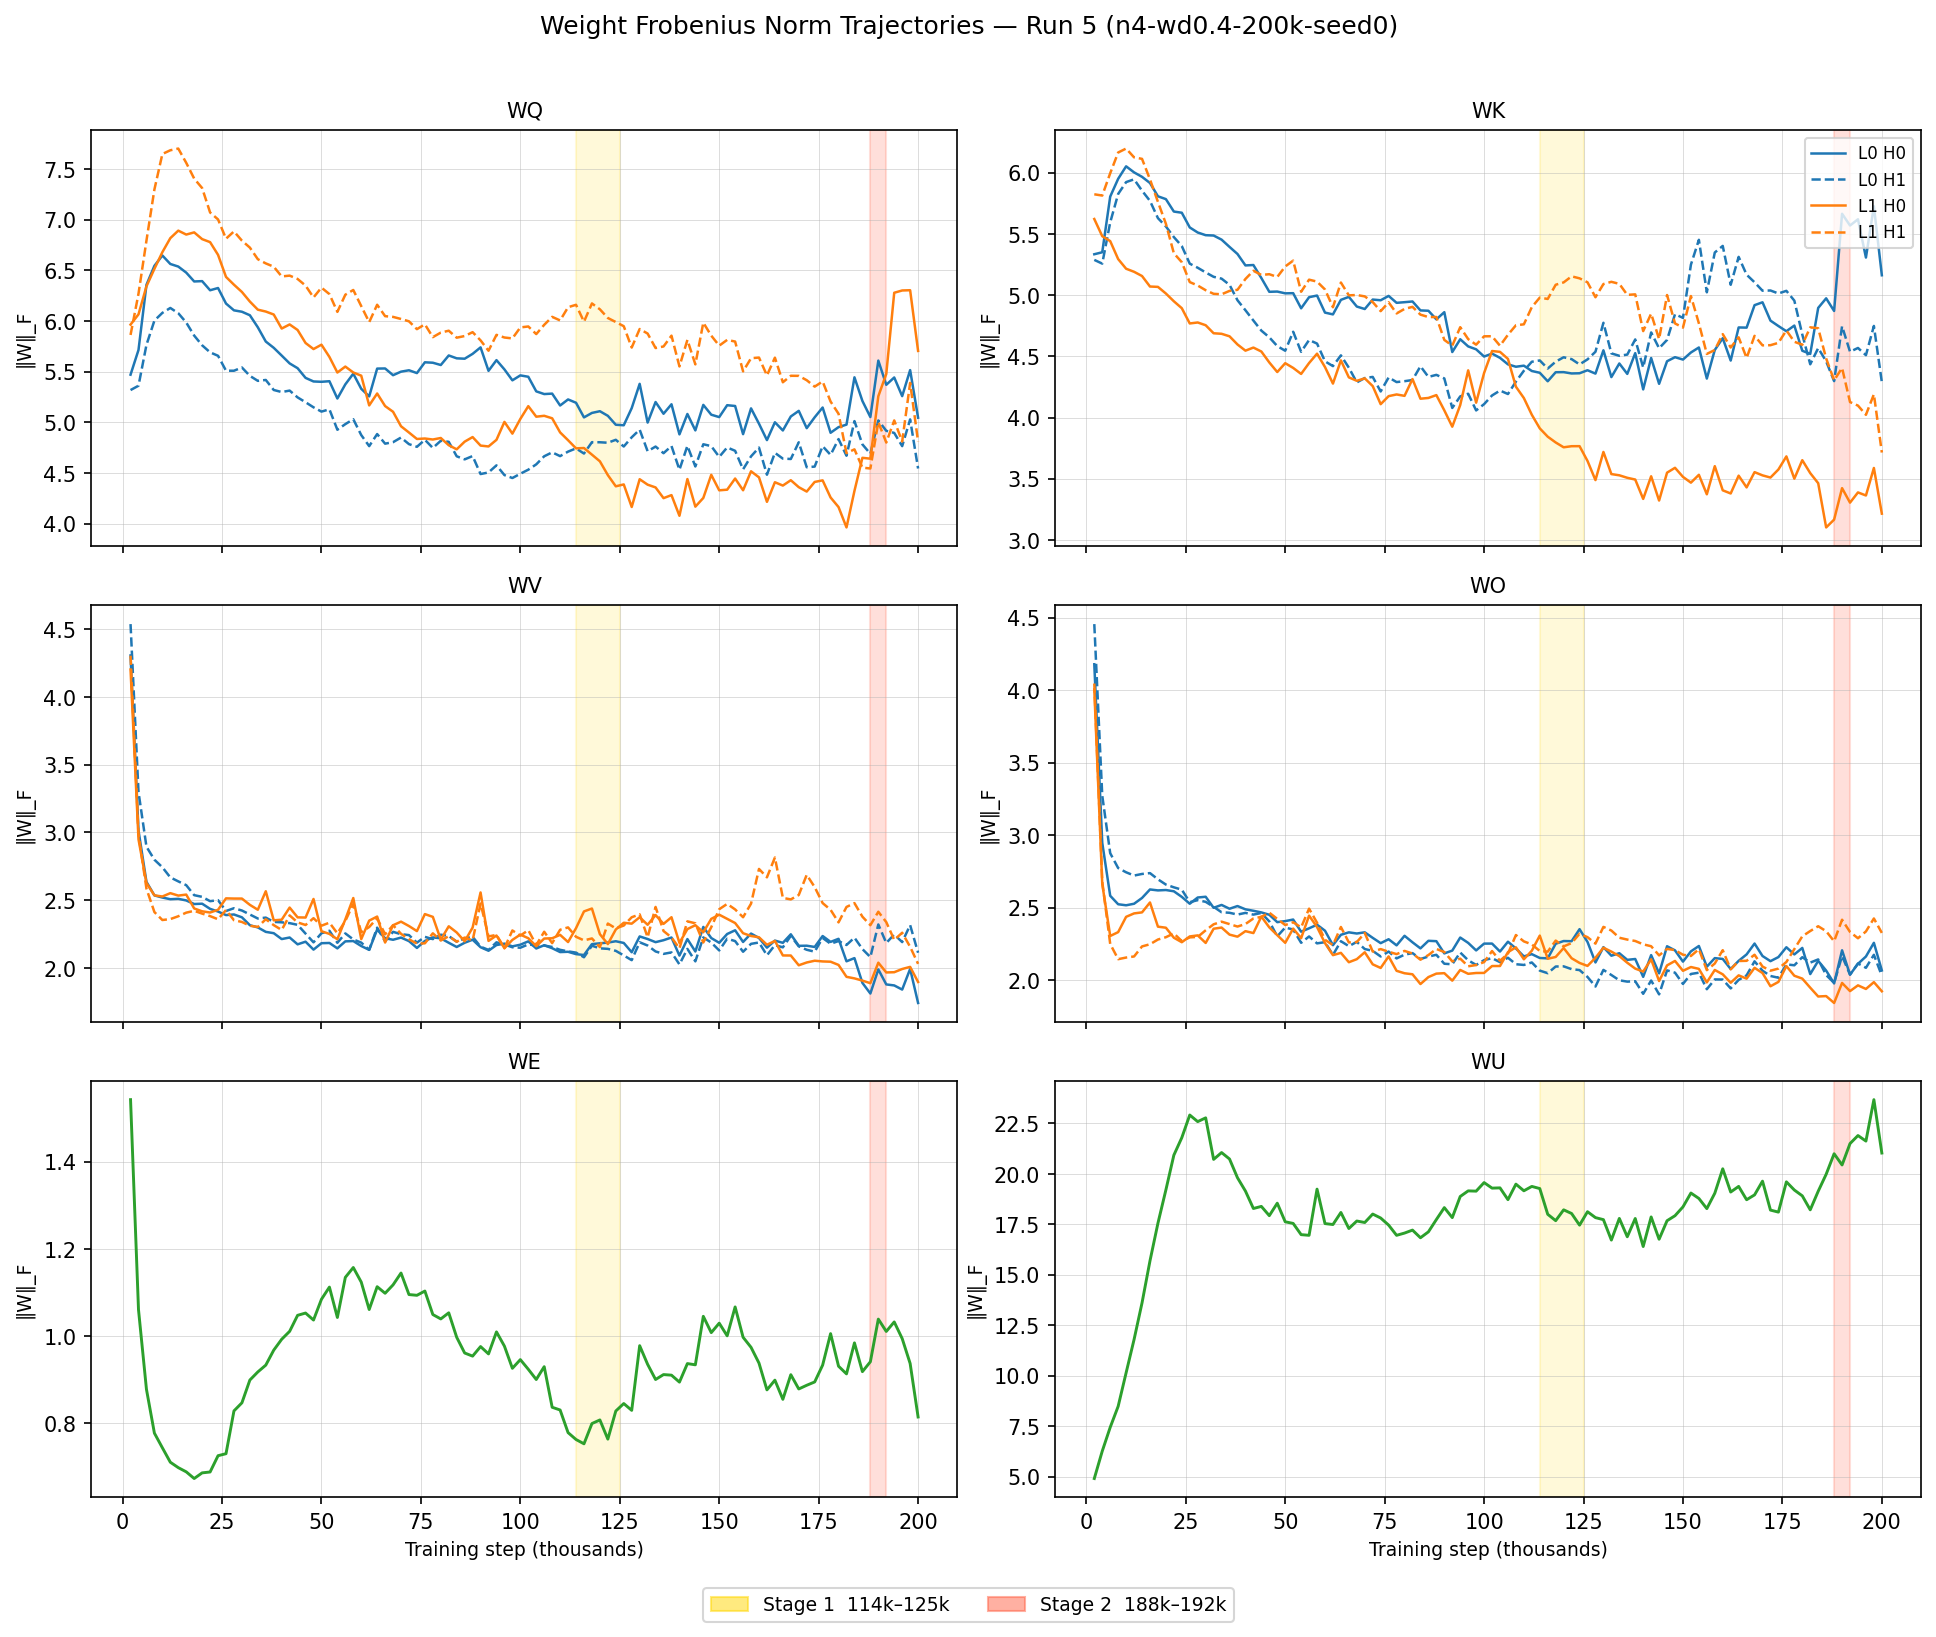
\includegraphics[width=\textwidth]{weight_norms.png}
\caption{Frobenius norm trajectories for all weight matrices over 200{,}000
  training steps (Run~5, \texttt{n4-wd0.4-200k-seed0}). Gold-shaded band:
  Stage~1 transition (114k--125k). Red-shaded band: Stage~2 transition
  (188k--192k). Blue lines: Layer~0 heads; orange lines: Layer~1 heads.
  Solid lines: Head~0; dashed lines: Head~1.}
\label{fig:weight-norms}
\end{figure}

Six patterns are visible in Figure~\ref{fig:weight-norms}:

\begin{enumerate}[noitemsep]
  \item \textbf{$W_U$ sharp rise at Stage~2.} The unembedding norm grows from
    $\sim$19.6 to $\sim$21.6 at the Stage~2 band --- the strongest signal in the
    plot. $W_U$ controls the sharpness of output class separation; sudden growth
    here means the model is differentiating output labels more aggressively,
    consistent with a circuit locking onto the correct algorithm.

  \item \textbf{$W_E$ rises at Stage~2.} Token embedding norm increases
    ($\sim$0.8$\to$$\sim$1.4 in the Stage~2 window), moving in concert with
    $W_U$. Embedding and unembedding strengthening simultaneously indicates the
    input$\to$output vocabulary pathway is being reinforced across both ends.

  \item \textbf{L1H0 $W_K$ monotone decline.} This head's key matrix decreases
    steadily from $\sim$4.4 at step 100k to $\sim$3.4 at step 196k, showing no
    response to either transition window. This is the clearest example of pure
    weight-decay compression in the data: the head is being uniformly suppressed
    throughout, suggesting its keys encode memorization-specific structure with no
    role in the generalizing algorithm.

  \item \textbf{L0H1 $W_K$ rises while L1H0 $W_K$ falls.} Two heads in
    different layers develop opposite norm trajectories under the same weight
    decay pressure: L0H1 $W_K$ grows from $\sim$4.1 to $\sim$5.4 between
    steps 30k and 160k. Two heads moving in opposite directions is inconsistent
    with smooth decay; it indicates one head being actively reinforced while the
    other is suppressed.

  \item \textbf{L1 $W_Q$ divergence at Stage~2.} In the $W_Q$ panel, L1H0
    (orange solid) and L1H1 (orange dashed) split sharply at the Stage~2 band:
    L1H0 rises from $\sim$4.7 to $\sim$6.3; L1H1 falls from $\sim$4.6 to
    $\sim$4.8. Both heads are in Layer~1. This is the primary candidate for a
    \emph{role swap} between the two Layer~1 heads at Stage~2; attention
    visualization (Section~\ref{sec:probes}) is the next tool to confirm or
    refute this.

  \item \textbf{Stage~1 is nearly invisible in weight space.} Despite producing
    a real $+7$ percentage-point accuracy improvement, Stage~1 shows no sharp
    inflections in any norm trajectory. All lines pass through the Stage~1 band
    with gradual, continuous slopes. This implies Stage~1 is not a
    weight-magnitude event --- the model's performance improved while weight
    norms changed minimally.
\end{enumerate}

\subsection{Stage 1: the direction hypothesis}
\label{sec:stage1-direction}

The Frobenius norm $\|W\|_F$ measures the \emph{magnitude} of a weight matrix
but is blind to its \emph{direction}. A weight matrix can rotate --- changing
which directions in input space it amplifies --- while keeping $\|W\|_F$
exactly constant. This is the direction hypothesis for Stage~1.

Formally: if $W_{t+\Delta t} \approx R W_t$ for some near-orthogonal $R \neq I$,
then $\|W_{t+\Delta t}\|_F = \|W_t\|_F$ but the head's functional behavior has
changed. The cosine similarity between flattened weight matrices at consecutive
checkpoints,
\[
  \cos(W_t,\, W_{t+\Delta t})
  = \frac{\langle \operatorname{vec}(W_t),\, \operatorname{vec}(W_{t+\Delta t})\rangle}
         {\|W_t\|_F\,\|W_{t+\Delta t}\|_F},
\]
would reveal a rotation as a drop toward zero. A diagnostic tool computing
this similarity across all 100 Run~5 checkpoints is planned as
\texttt{src/interp/weight\_cosine.py}.

\subsection{Probe inputs for attention visualization}
\label{sec:probes}

Attention patterns are computed fresh for every input: the same head produces
completely different patterns on different inputs. Probe design is hypothesis
control --- a carefully chosen input makes the head's algorithm legible, while
a random input may be dominated by padding or coincidental structure.

Three properties define a good probe for this task: (1) \textbf{structural
clarity} --- a minimal graph with an unambiguous ground-truth answer;
(2) \textbf{discriminative contrast} --- pairs differing in exactly one
structural feature; (3) \textbf{edge-order variation} --- the same graph
with different edge orderings, to separate content-driven attention from
position-driven attention.

Six specific probes are defined for 4-node graphs (nodes 0, 1, 2, 3):

\begin{table}[H]
\centering
\small
\begin{tabular}{@{}clccp{4.2cm}@{}}
\toprule
\# & Graph edges & Query & Answer & What it tests \\
\midrule
P1 & $(0{\to}1),(1{\to}2),(2{\to}3)$ & src=0, dst=3 & 3 &
  Single linear path --- does head attend to all path edges? \\[3pt]
P2 & $(0{\to}3),(0{\to}1),(1{\to}2)$ & src=0, dst=3 & 1 &
  Direct edge exists --- does head find the shortcut? \\[3pt]
P3 & $(1{\to}0),(2{\to}1),(3{\to}2)$ & src=0, dst=3 & INF &
  \textbf{Edges reversed} --- does attention collapse, revealing that the
  model understands edge directionality? \\[3pt]
P4 & P1 edges in reverse order & src=0, dst=3 & 3 &
  \textbf{Same graph, different positions} --- if pattern matches P1, head
  is content-driven; if different, it is position-driven. \\[3pt]
P5 & $(0{\to}1),(1{\to}3),(0{\to}2),(2{\to}3)$ & src=0, dst=3 & 2 &
  Two equal-length paths --- does head split attention or specialize? \\[3pt]
P6 & $(0{\to}1),(1{\to}2),(2{\to}3)$ & src=0, dst=1 & 1 &
  Same graph as P1, closer destination --- does attention re-orient to query? \\
\bottomrule
\end{tabular}
\caption{Six probe inputs for attention visualization. P3 tests edge
  directionality --- the core novelty of this task. P4 determines whether
  any attention-pattern conclusions are position-confounded; if patterns
  differ between P1 and P4, all head-pattern conclusions require re-examination.
  All six probes are evaluated at steps 126k, 190k, and 196k.}
\end{table}

\subsection{Attention visualization: initial findings}
\label{sec:attn-findings}

The full 6-probe $\times$ 3-checkpoint $\times$ 4-head grid was computed using
\texttt{attention\_viz.py} and saved as \texttt{notebooks/attention\_patterns.png}
(Figure~\ref{fig:attn-full}). A single-checkpoint zoom at step~190k
(Stage~2 transition peak) is in \texttt{notebooks/attention\_190k\_zoom.png}
(Figure~\ref{fig:attn-190k}).

\begin{figure}[H]
\centering
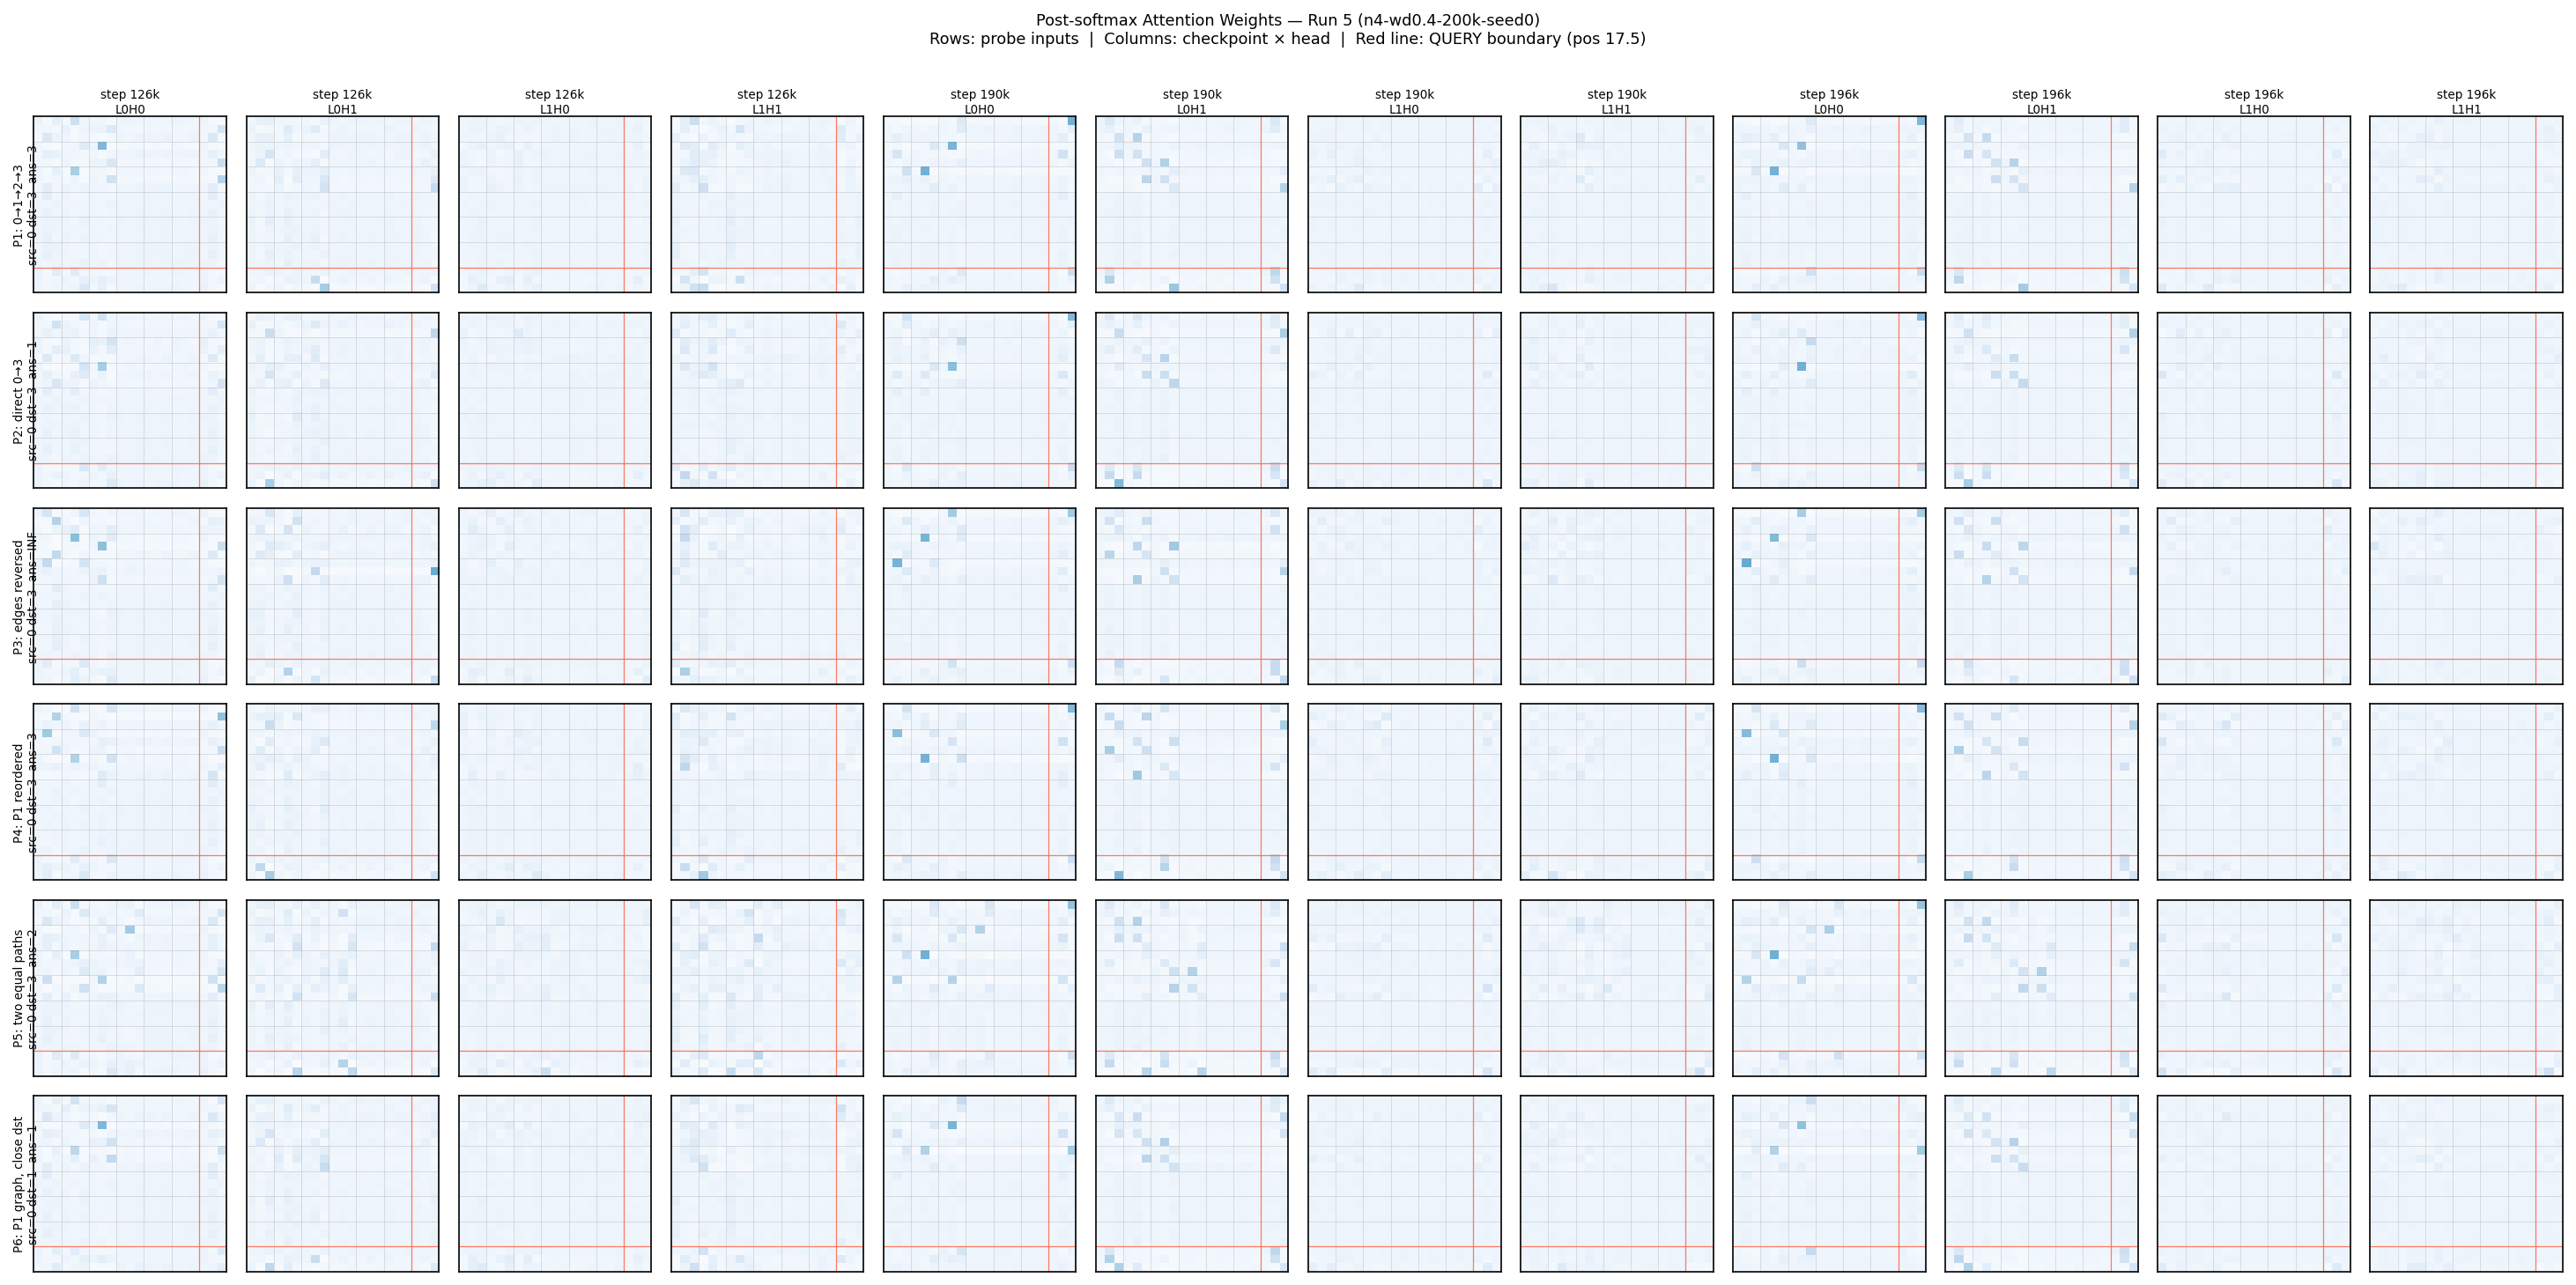
\includegraphics[width=\textwidth]{attention_patterns.png}
\caption{Post-softmax attention weights for all six probes at steps 126k, 190k,
  and 196k. Columns are grouped as checkpoint $\times$ head (L0H0, L0H1, L1H0,
  L1H1 per checkpoint). Gray lines mark 3-token EDGE triplet boundaries; red
  line marks the QUERY boundary at position 17.5. Color scale: 0 (white) to
  1 (dark blue), shared across all cells.}
\label{fig:attn-full}
\end{figure}

\begin{figure}[H]
\centering
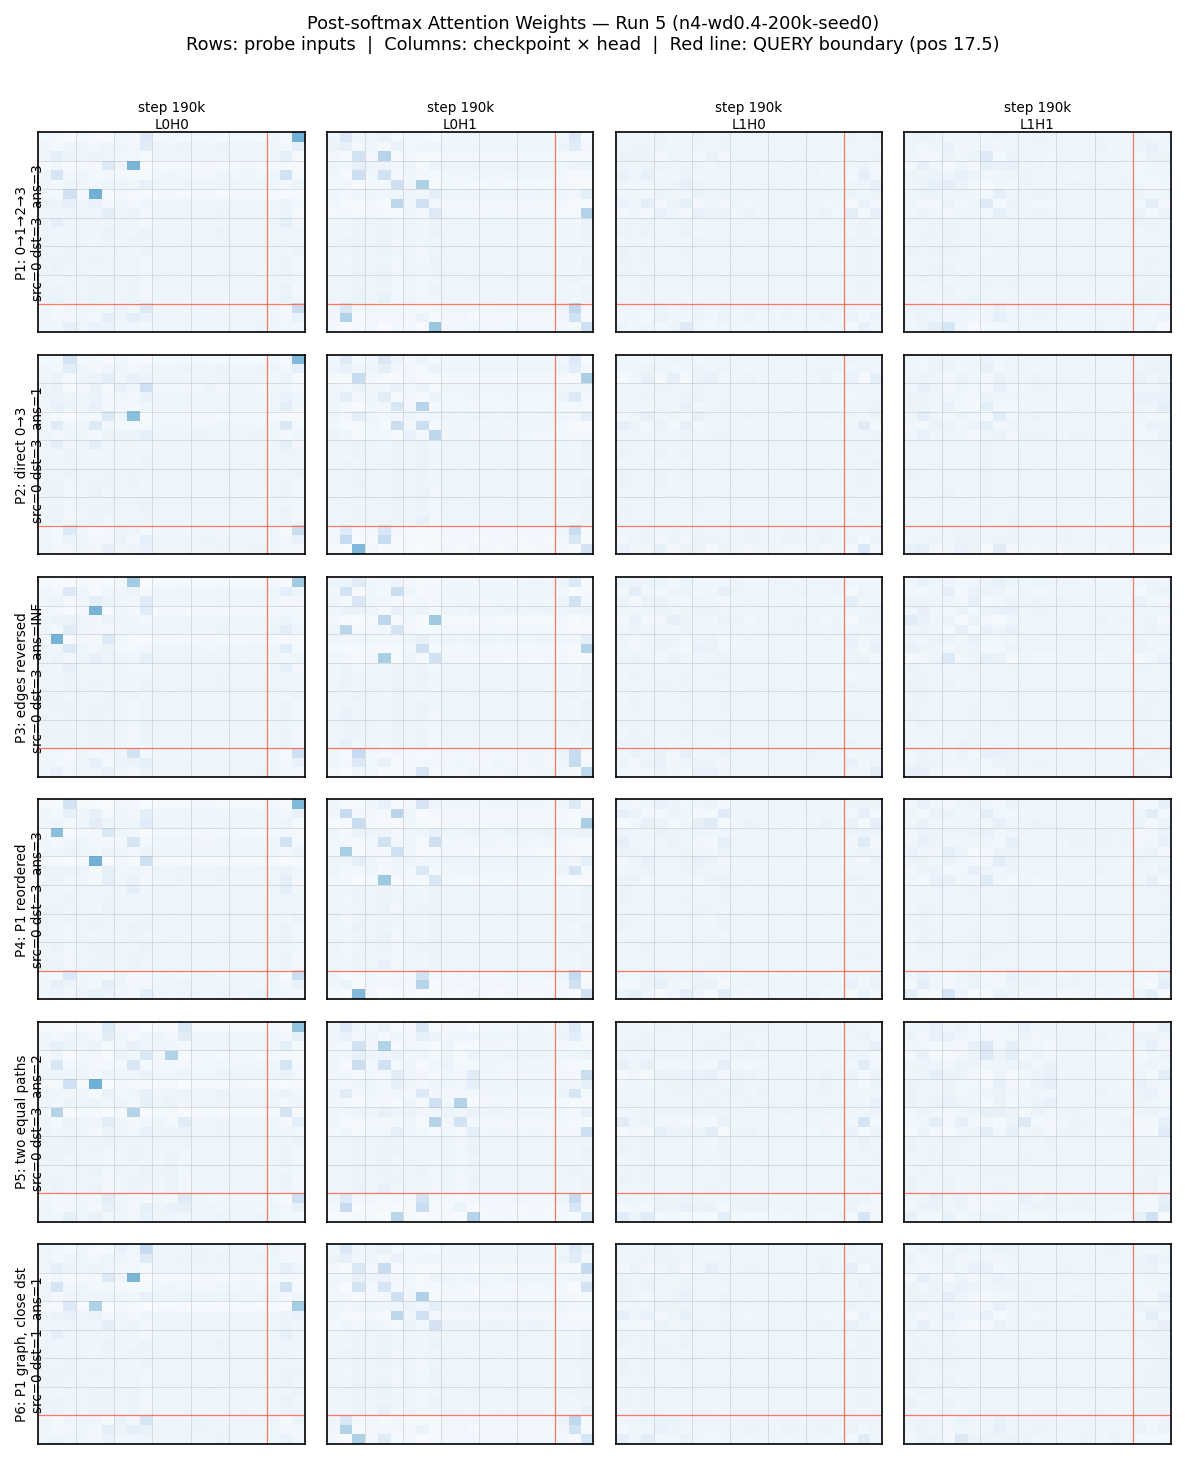
\includegraphics[width=0.85\textwidth]{attention_190k_zoom.png}
\caption{Zoom: step~190k (Stage~2 transition peak), all four heads, all six
  probes. At this checkpoint the L1H0/L1H1 WQ norm divergence from
  Figure~\ref{fig:weight-norms} is at its maximum.}
\label{fig:attn-190k}
\end{figure}

Three observations emerge from the initial grid.

\paragraph{Observation 1: L0H0 is the primary information-gathering head.}
L0H0 shows sharp, sparse attention patterns that vary systematically across
probe inputs. The bright spots --- individual query positions attending to a
small number of key positions at high weight --- change when the probe graph
changes. This is the signature of a head that is actively reading specific
edges from the sequence. L0H1 also shows structure but is more diffuse:
lighter and spread across more positions, suggesting a softer aggregation role.

\paragraph{Observation 2: L1 heads are near-uniform across all probes and
checkpoints.}
L1H0 and L1H1 both exhibit near-uniform attention at steps 126k, 190k, and
196k: attention mass is spread nearly evenly across all key positions,
regardless of probe input. For an attention-only model, near-uniform attention
means that head's output is approximately a fixed learned weighted average of
all residual-stream vectors --- not selective reading. This raises the
question of what role L1 plays: if it is not selecting specific tokens, its
contribution must be in the \emph{value} computation (what it reads and writes
back via $W_V$ and $W_O$) rather than the \emph{query-key} routing (which
positions to attend to). This is called the OV circuit hypothesis and is
the primary open question for Layer~1.

\paragraph{Observation 3: L0H0 shows a directionality signal in P1 vs.\ P3.}
The bright-spot locations in L0H0 shift between probe P1 (linear path
$0{\to}1{\to}2{\to}3$, answer~3) and probe P3 (same edges reversed,
$1{\to}0,\;2{\to}1,\;3{\to}2$, answer~INF). Because P1 and P3 encode the
same node tokens at the same sequence positions but with source and destination
swapped within each EDGE triplet, this shift is preliminary evidence that L0H0
encodes edge direction. A quantitative test is the next planned analysis step.

\subsubsection{Quantitative probe comparison: directionality and position vs.\ content}
\label{sec:probe-comparison}

The metric used is \textbf{symmetric KL divergence} and \textbf{cosine similarity}
between the QUERY-row attention submatrices of two probes, for one head at one
checkpoint. ``QUERY rows'' are positions 18--20 — the $[\text{QUERY},
\text{src}, \text{dst}]$ triplet — because those are the positions whose
attention patterns encode which edges the model uses to route toward its answer.

For a single query row (a 21-dim probability vector from softmax), the symmetric
KL is $\frac{1}{2}[\text{KL}(P\|Q) + \text{KL}(Q\|P)]$, averaged over the three
QUERY rows.  Cosine similarity is computed over the flattened $3 \times 21 = 63$
vector.  Interpretation: \textbf{high KL + low cosine} = the two probes produce
fundamentally different attention patterns in that head; \textbf{low KL + high
cosine} = the head is insensitive to the difference between the two probes.

For the position-vs-content test specifically: P1 and P4 encode identical edges
in reversed sequence order.  A \emph{content-driven} head follows the edge values
as they move, producing different patterns (high KL, low cosine).  A
\emph{position-driven} head attends to fixed slots regardless of content,
producing nearly identical patterns (low KL, high cosine).

\begin{table}[H]
\centering
\small
\begin{tabular}{@{}lcccccc@{}}
\toprule
 & \multicolumn{2}{c}{step 126k} & \multicolumn{2}{c}{step 190k} & \multicolumn{2}{c}{step 196k} \\
\cmidrule(lr){2-3}\cmidrule(lr){4-5}\cmidrule(lr){6-7}
Comparison & KL & cos & KL & cos & KL & cos \\
\midrule
P1 vs P3 \;L0H0\; (directionality)  & 0.207 & 0.802 & 0.136 & 0.871 & 0.147 & 0.837 \\
P1 vs P4 \;L0H0\; (pos vs content)  & 0.139 & 0.876 & 0.090 & 0.915 & 0.206 & 0.811 \\
\midrule
P1 vs P3 \;L0H1\; (directionality)  & 0.426 & 0.593 & 0.602 & 0.601 & 0.459 & 0.633 \\
P1 vs P4 \;L0H1\; (pos vs content)  & 0.354 & 0.561 & 0.692 & 0.493 & 0.538 & 0.535 \\
\midrule
P1 vs P3 \;L1H0\; (directionality)  & 0.079 & 0.915 & 0.068 & 0.926 & 0.095 & 0.895 \\
P1 vs P4 \;L1H0\; (pos vs content)  & 0.034 & 0.963 & 0.048 & 0.954 & 0.045 & 0.958 \\
\midrule
P1 vs P3 \;L1H1\; (directionality)  & 0.293 & 0.738 & 0.079 & 0.913 & 0.034 & 0.969 \\
P1 vs P4 \;L1H1\; (pos vs content)  & 0.122 & 0.890 & 0.095 & 0.918 & 0.047 & 0.955 \\
\bottomrule
\end{tabular}
\caption{Symmetric KL divergence and cosine similarity between probe pairs,
  measured on QUERY-row attention distributions (positions 18--20) for each
  head. High KL / low cosine = the head distinguishes the two probes. The
  directionality test compares P1 ($0{\to}1{\to}2{\to}3$, answer~3) with P3
  (edges reversed, answer~INF). The position-vs-content test compares P1 with
  P4 (same edges, reversed sequence order, same answer).}
\label{tab:probe-comparison}
\end{table}

Four findings emerge from Table~\ref{tab:probe-comparison}.

\paragraph{Finding 1: L0H1, not L0H0, carries the strongest directionality and
content signal.}
L0H1 has the highest KL values across both tests and the lowest cosine
similarities.  At step~190k its directionality KL reaches 0.602 and its
position-vs-content cosine falls to 0.493 --- nearly orthogonal, meaning P1 and
P4 produce almost completely different QUERY-row patterns.  The visual analysis
(Section~\ref{sec:attn-findings}) suggested L0H0 was primary because it appeared
sharper; the quantitative analysis reveals that L0H1's diffuse-looking patterns
are in fact more sensitive to semantic structure.  L0H1 is \emph{content-driven}:
it follows edge values as they move in the sequence rather than attending to fixed
positional slots.

\paragraph{Finding 2: L0H0 shows a mixed, moderate signal.}
L0H0's directionality KL (~0.14--0.21) and position-vs-content KL (~0.09--0.21)
are in a similar range to each other, with no clean separation.  This is
consistent with a head that performs a joint function of both position and content
--- the score $\text{score}(q, k) = q W_Q W_K^\top k$ mixes positional and token
information unless $W_Q$/$W_K$ perfectly disentangle them.

\paragraph{Finding 3: L1H0 is strongly position-invariant.}
L1H0's position-vs-content cosine stays at 0.95--0.96 across all three
checkpoints.  Reordering the edges has almost no effect on its QUERY-row
attention.  Combined with the near-uniform visual pattern, L1H0's QUERY-row
computation is essentially a fixed function of the query token's position, not
the edge content.  This is the quantitative confirmation that L1H0 is not doing
selective edge-reading.

\paragraph{Finding 4: L1H1 lost its sensitivity at Stage~2.}
At step~126k L1H1 has a non-trivial directionality KL of 0.293.  By step~196k
(post-Stage~2) both its directionality KL (0.034) and its position-vs-content KL
(0.047) are near zero, with cosines above 0.95.  Stage~2 drove L1H1 toward
complete probe-insensitivity --- a concrete signature of the L1H0/L1H1 role
divergence visible in the WQ norm plot (Figure~\ref{fig:weight-norms}).

\paragraph{Synthesis.}
The grokking transition at Stage~2 corresponds to a functional reorganization of
Layer~1: L1H1 loses its directionality sensitivity entirely while L1H0 settles
into a strongly position-invariant role.  Meanwhile L0H1, despite appearing
diffuse in the attention heatmaps, is the head most sensitive to both edge
direction and edge content --- a finding that only emerged from the quantitative
comparison and would have been missed by visual inspection alone.  The model
distributes graph reasoning across its four heads in a non-obvious way: Layer~0
handles content-sensitive reading (with L0H1 as the primary semantic head and
L0H0 playing a mixed role), while Layer~1's contribution after Stage~2 appears
to lie in what it writes to the residual stream rather than where it attends.
This motivates the OV circuit analysis as the next step.

\subsubsection{OV circuit analysis: findings}
\label{sec:ov-findings}

The full token-to-logit OV matrix $W_E W_V W_O W_U \in \mathbb{R}^{|\mathcal{V}| \times |\mathcal{V}|}$
was computed for all four heads at steps 126k, 190k, and 196k.
Figure~\ref{fig:ov-circuits} shows the 8$\times$8 heatmaps and the 196k$-$126k
difference row; Table~\ref{tab:ov-norms} gives the Frobenius norms.

\begin{figure}[H]
\centering
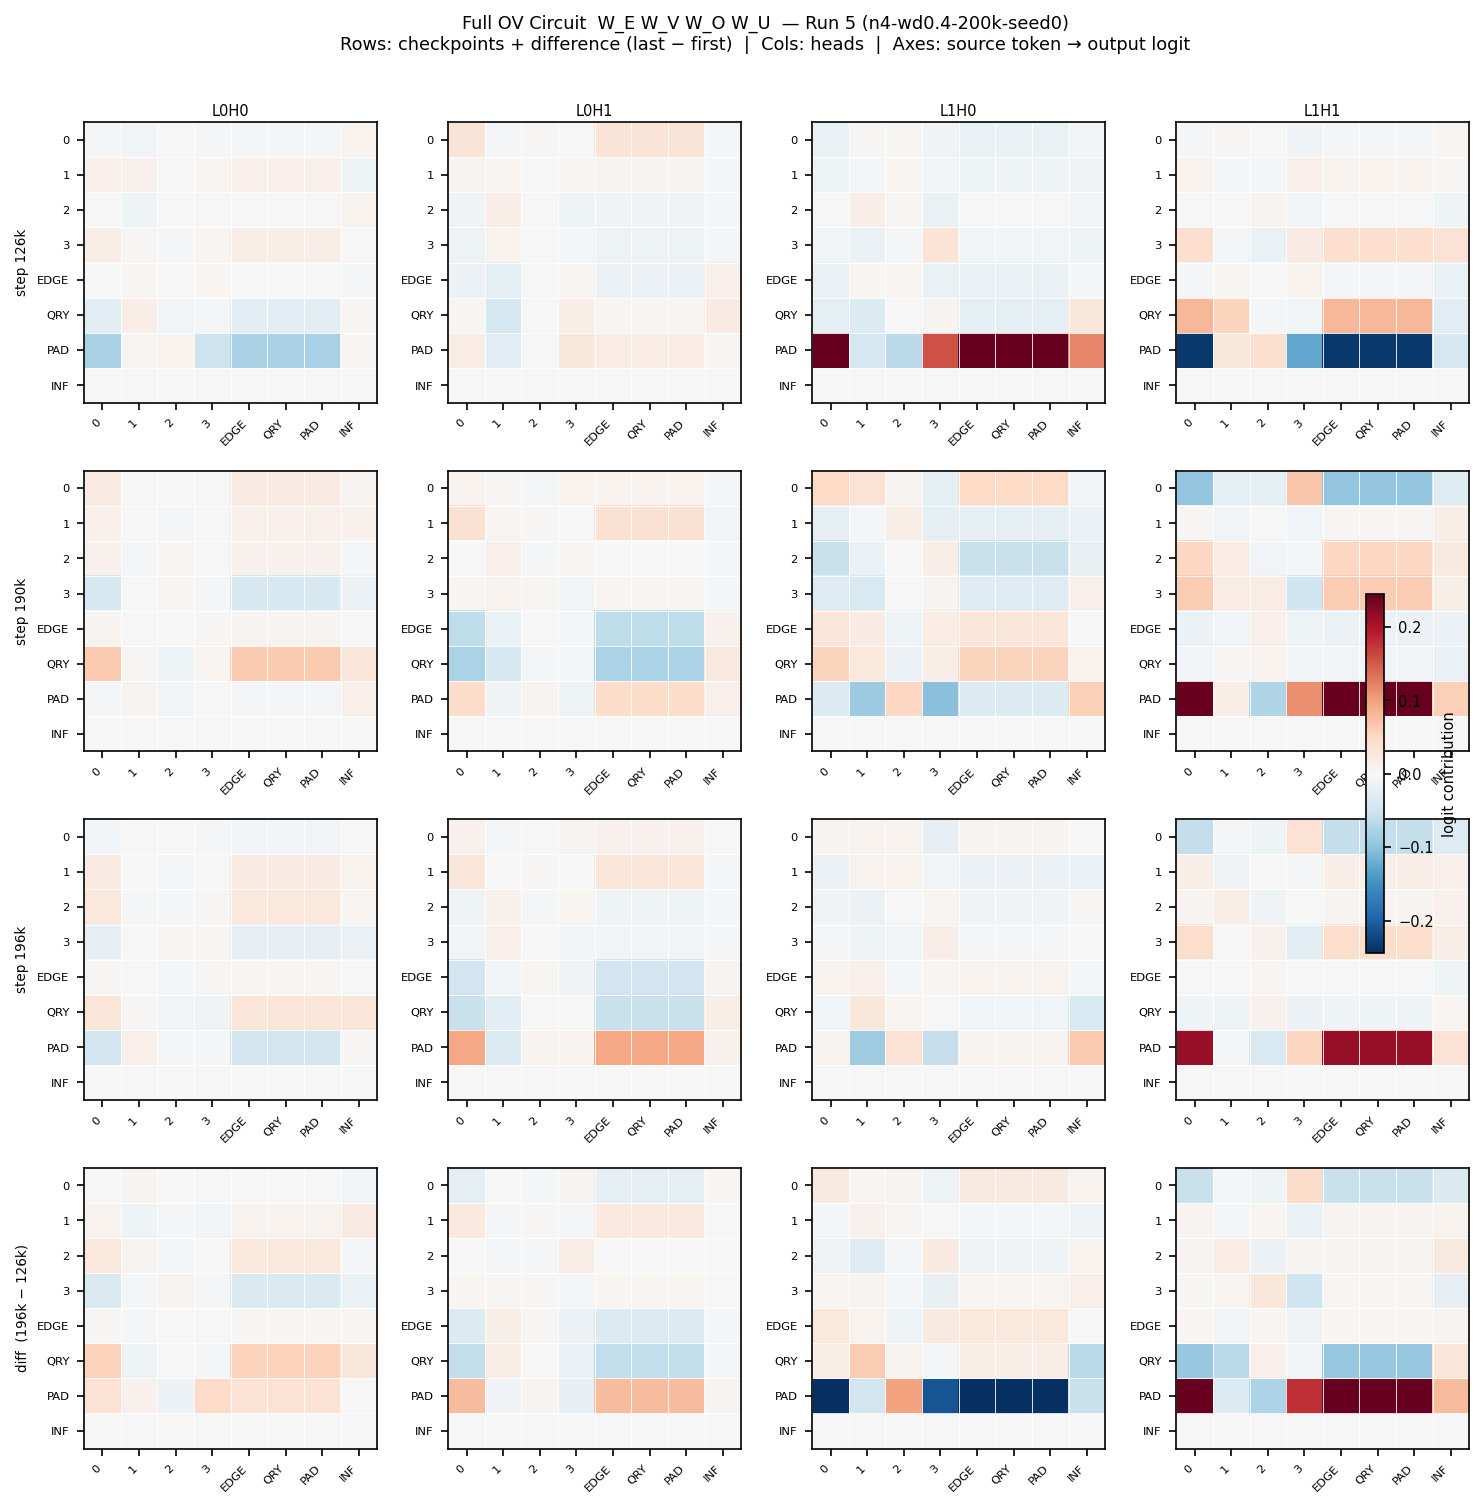
\includegraphics[width=\textwidth]{ov_circuits.png}
\caption{Full OV circuit matrices $W_E W_V W_O W_U$ for all four heads at
  steps 126k, 190k, and 196k, plus the difference (196k $-$ 126k).
  y-axis: source token (what is being attended to); x-axis: output logit.
  Diverging colormap: red = positive contribution, blue = negative.
  The PAD row dominates L1H0 and L1H1 at step~126k and largely disappears
  by step~196k.}
\label{fig:ov-circuits}
\end{figure}

\begin{table}[H]
\centering
\small
\begin{tabular}{@{}lcccccc@{}}
\toprule
Head & $\|OV_{126k}\|_F$ & $\|OV_{190k}\|_F$ & $\|OV_{196k}\|_F$
     & $\|\Delta OV\|_F$ & rel.\ change \\
\midrule
L0H0 & 0.183 & 0.165 & 0.139 & 0.173 & 0.94$\times$ \\
L0H1 & 0.112 & 0.237 & 0.255 & 0.221 & \textbf{1.98$\times$} \\
L1H0 & \textbf{0.576} & 0.281 & 0.149 & 0.583 & 1.01$\times$ \\
L1H1 & 0.531 & 0.651 & 0.461 & 0.952 & 1.79$\times$ \\
\bottomrule
\end{tabular}
\caption{Frobenius norms of the full OV circuit matrix at each checkpoint.
  $\|\Delta OV\|_F = \|OV_{196k} - OV_{126k}\|_F$.  Relative change is
  $\|\Delta OV\|_F / \|OV_{126k}\|_F$.  L1H0 starts with the largest OV
  circuit and undergoes the most dramatic collapse; L0H1 nearly doubles.}
\label{tab:ov-norms}
\end{table}

Four findings emerge.

\paragraph{Finding 5: L1H0's OV circuit was primarily a PAD-token bias and
Stage~2 eliminated it.}
At step~126k, L1H0's OV matrix shows a uniformly saturated positive row for
the PAD source token --- the PAD row dwarfs all others.  Because all PAD tokens
share the same embedding, attending to any PAD position produces the same value
vector.  Near-uniform attention over a sequence with $\sim$43\% PAD positions
(9 of 21 for a 3-edge graph) therefore injects a large constant offset into the
residual stream, regardless of the actual graph.  This is a learned bias
disguised as attention.  By step~196k the PAD row is nearly gone ($\|OV\|_F$
drops from 0.576 to 0.149), and the difference heatmap shows deep blue on the
PAD row.  Stage~2 was the point at which the model stopped relying on this
shortcut.

\paragraph{Finding 6: L1H1 was the negative counterpart to L1H0's PAD bias.}
L1H1's PAD row at step~126k is strongly negative (deep blue), the opposite sign
of L1H0's.  The two heads were jointly injecting a PAD-driven offset
(L1H0 positive, L1H1 negative); the net effect was a structured but
opaque bias term encoded in the difference of two large cancelling circuits.
After Stage~2 both circuits restructure, with L1H1's difference norm (0.952)
exceeding L1H0's (0.583) --- indicating a complex redistribution, not simply
zeroing out.

\paragraph{Finding 7: L0H1's OV circuit nearly doubled at Stage~2.}
L0H1's $\|OV\|_F$ grows from 0.112 to 0.255 (1.98$\times$) --- the only head
whose OV circuit strengthens substantially.  This is the OV-side complement of
Finding~1 (L0H1 is the most semantically sensitive head in the QK analysis):
Stage~2 simultaneously made L0H1's attention routing more content-sensitive
\emph{and} amplified what it writes when it attends.

\paragraph{Revised Stage~2 picture.}
Stage~2 is a functional redistribution across all four heads.  Before Stage~2,
Layer~1 is dominated by a large PAD-token OV bias (L1H0 positive, L1H1
negative) that likely acts as a coarse constant correction to the output
distribution.  After Stage~2, this PAD-bias is dismantled and replaced by a
more structured computation: L0H1's OV circuit grows, its QK routing becomes
more content-sensitive, and Layer~1 settles into a low-norm, nearly uniform
state.  The grokking accuracy jump corresponds to the model abandoning a
shortcut (constant PAD-based offset) and generalizing via a proper
content-sensitive circuit concentrated in L0H1.

\subsubsection{Stage 1 OV circuit and probe comparison analysis}
\label{sec:stage1-analysis}

The same analyses were run on the Stage~1 window (steps 100k, 116k, 126k) to
determine whether Stage~1 is also an OV-circuit event, and why it was invisible
in the individual weight-norm trajectories.

\begin{table}[H]
\centering
\small
\begin{tabular}{@{}lcccccc@{}}
\toprule
Head & $\|OV_{100k}\|_F$ & $\|OV_{116k}\|_F$ & $\|OV_{126k}\|_F$
     & $\|\Delta OV\|_F$ & rel.\ change \\
\midrule
L0H0 & 0.085 & \textbf{0.221} & 0.183 & 0.175 & 2.04$\times$ \\
L0H1 & 0.216 & 0.159 & 0.112 & 0.177 & 0.82$\times$ (shrank) \\
L1H0 & 0.295 & 0.524 & \textbf{0.576} & 0.609 & \textbf{2.06$\times$} \\
L1H1 & 0.364 & 0.618 & 0.531 & 0.418 & 1.15$\times$ \\
\bottomrule
\end{tabular}
\caption{OV circuit Frobenius norms across Stage~1.  L1H0 and L1H1 both grow
  substantially, the opposite direction from Stage~2.  L0H0 spikes at the
  transition onset (116k) then retreats.  L0H1 shrinks throughout.}
\label{tab:ov-norms-stage1}
\end{table}

\begin{figure}[H]
\centering
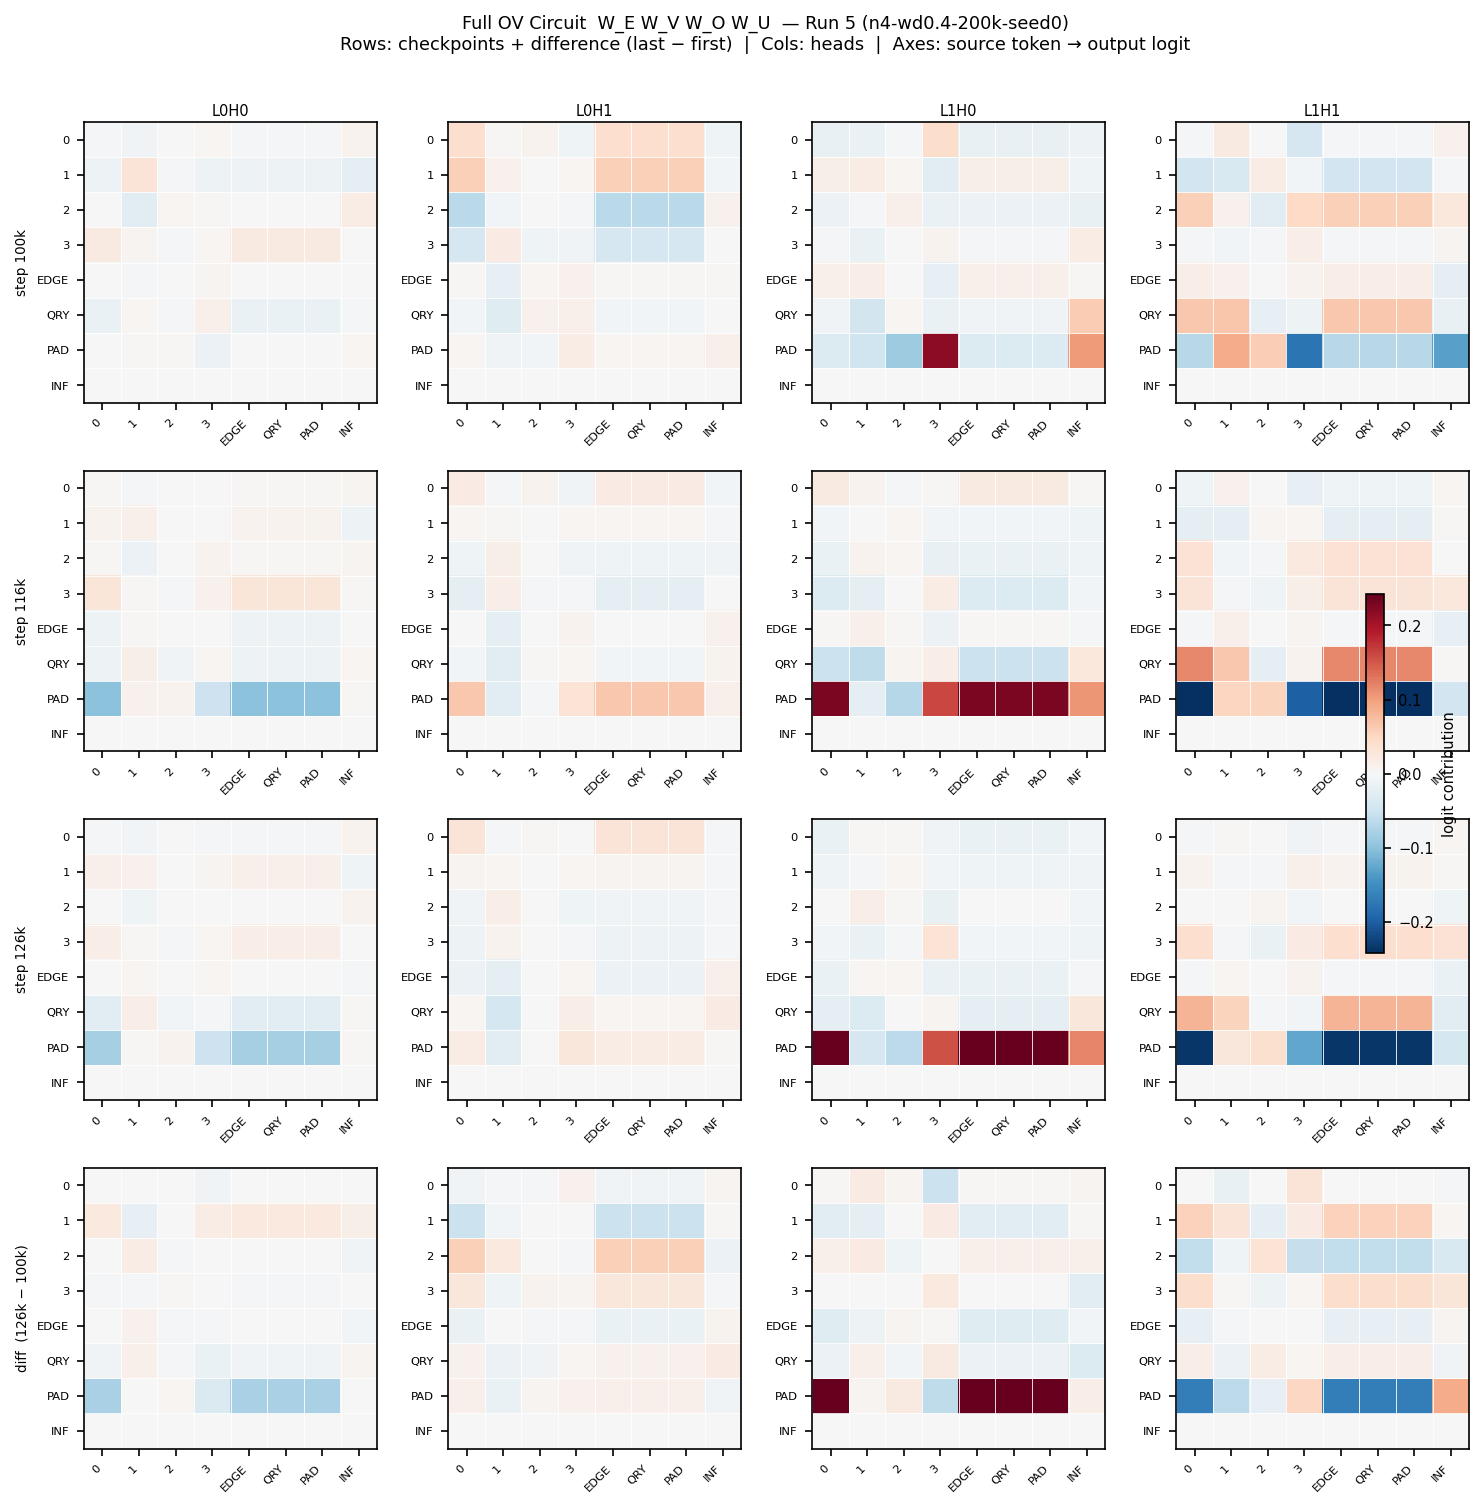
\includegraphics[width=\textwidth]{ov_circuits_stage1.png}
\caption{OV circuit matrices at steps 100k, 116k, 126k, and the 126k$-$100k
  difference.  The PAD row in L1H0 grows from a single bright cell (100k) into
  a full saturated band (116k), confirming the PAD-bias shortcut is built during
  Stage~1.  L1H1's negative PAD row forms simultaneously.}
\label{fig:ov-stage1}
\end{figure}

\begin{table}[H]
\centering
\small
\begin{tabular}{@{}lcccccc@{}}
\toprule
 & \multicolumn{2}{c}{step 100k} & \multicolumn{2}{c}{step 116k} & \multicolumn{2}{c}{step 126k} \\
\cmidrule(lr){2-3}\cmidrule(lr){4-5}\cmidrule(lr){6-7}
Comparison & KL & cos & KL & cos & KL & cos \\
\midrule
P1 vs P3 \;L0H0\; (directionality)  & 0.301 & 0.687 & 0.155 & 0.844 & 0.207 & 0.802 \\
P1 vs P4 \;L0H0\; (pos vs content)  & 0.193 & 0.857 & 0.132 & 0.876 & 0.139 & 0.876 \\
\midrule
P1 vs P3 \;L0H1\; (directionality)  & 0.351 & 0.638 & 0.466 & 0.632 & 0.426 & 0.593 \\
P1 vs P4 \;L0H1\; (pos vs content)  & 0.495 & 0.484 & 0.549 & 0.511 & 0.354 & 0.561 \\
\midrule
P1 vs P3 \;L1H0\; (directionality)  & 0.181 & 0.813 & 0.093 & 0.909 & 0.079 & 0.915 \\
P1 vs P4 \;L1H0\; (pos vs content)  & 0.041 & 0.965 & 0.047 & 0.948 & 0.034 & 0.963 \\
\midrule
P1 vs P3 \;L1H1\; (directionality)  & 0.442 & 0.611 & 0.571 & 0.485 & 0.293 & 0.738 \\
P1 vs P4 \;L1H1\; (pos vs content)  & 0.130 & 0.914 & 0.177 & 0.900 & 0.122 & 0.890 \\
\bottomrule
\end{tabular}
\caption{Probe comparison table across Stage~1.  Compare with
  Table~\ref{tab:probe-comparison} for Stage~2.  L0H0 loses directional
  sensitivity at Stage~1; L0H1 gains it.  L1H1 shows a transient peak in
  directionality KL at 116k.}
\label{tab:probe-stage1}
\end{table}

Four findings are specific to Stage~1.

\paragraph{Finding 8: Stage~1 and Stage~2 are symmetric events — Stage~1 builds
the PAD-bias shortcut that Stage~2 dismantles.}
L1H0's OV norm grows from 0.295 to 0.576 across Stage~1 (2.06$\times$), the
exact reverse of its 0.576$\to$0.149 collapse at Stage~2.  The OV figure
(Figure~\ref{fig:ov-stage1}) shows the PAD row in L1H0 forming during Stage~1:
at step~100k there is only a single bright cell; by step~116k the full saturated
red band is present.  L1H1's opposing negative PAD row forms simultaneously.
The model first discovered a coarse shortcut (inject a constant PAD-based
offset), used it to bootstrap a first generalization step, and then eventually
found a proper content-sensitive algorithm to replace it.

\paragraph{Finding 9: Stage~1 is invisible in individual weight norms because
it is a matrix-alignment event.}
Individual W\textsubscript{V} and W\textsubscript{O} norms barely changed across
Stage~1 (confirmed by the flat weight-norm trajectories at the 114k--125k band in
Figure~\ref{fig:weight-norms}).  Yet the OV product
$\|W_{E} W_V W_O W_U\|_F$ grew 2$\times$.  This is possible because
$\|AB\|_F \leq \|A\|_F\|B\|_F$: two matrices can become better-aligned ---
the right singular vectors of $W_V$ rotating to match the left singular vectors
of $W_O$ --- doubling their product's norm while leaving both individual norms
unchanged.  Stage~1 is thus a \emph{weight-rotation event} confined to the
$W_V$/$W_O$ subspace of Layer~1; the individual-norm view was genuinely blind to
it, not merely coarse-grained.

\paragraph{Finding 10: L0H0 loses directional sensitivity at Stage~1.}
L0H0's directionality KL falls from 0.301 to 0.155 at Stage~1 onset.  The head
becomes less able to distinguish P1 from P3 as the model's accuracy improves.
This is coherent: L0H0 is partially offloading its directional role to the
PAD-bias shortcut being constructed in Layer~1, allowing Layer~0 to shift
toward a more position-anchored reading strategy.

\paragraph{Finding 11: L1H1 shows a transient directionality peak at Stage~1
onset.}
L1H1's directionality KL spikes to 0.571 (cosine 0.485) at step~116k, the
highest it reaches in the entire 100k--196k range, then retreats to 0.293 by
126k.  This transient signal at the exact onset of the transition is consistent
with a head in mid-reorganization: briefly expressing content-sensitive behavior
before its final role as the negative counterpart to L1H0's PAD bias is
established.

\paragraph{Unified two-stage picture.}
The two grokking transitions are now mechanistically interpretable as a single
lifecycle of a shortcut:
\begin{enumerate}
  \item \textbf{Stage~1 (114k--126k):} Layer~1 builds a PAD-token OV bias
    (L1H0 positive, L1H1 negative).  The bias acts as a constant correction to
    the output distribution that improves accuracy without requiring the model to
    properly read graph structure.  This is a matrix-alignment event invisible to
    per-weight Frobenius norms.  L0H0 offloads some of its directional role;
    L0H1 gains directional sensitivity.
  \item \textbf{Stage~2 (188k--192k):} Layer~1's PAD-bias is dismantled.
    L0H1's OV circuit simultaneously doubles and its QK routing becomes more
    content-sensitive.  The shortcut is replaced by a proper content-sensitive
    circuit concentrated in L0H1.  The second, larger accuracy jump corresponds
    to this replacement.
\end{enumerate}
The model's path through weight space is: memorize $\to$ shortcut
(Stage~1) $\to$ proper generalization (Stage~2).  This is a three-phase grokking
trajectory, not a single phase transition as in the original Power et al.\
framing.

\subsubsection{PAD-position ablation: causal validation}
\label{sec:pad-ablation}

The correlation evidence above identifies the PAD-token OV bias as the Stage~1
shortcut. To test this causally, we zero the attention weight columns
corresponding to PAD key positions in Layer~1 before value aggregation, and
measure validation accuracy at four checkpoints spanning the full trajectory.
Two ablation variants are tested:

\begin{description}[noitemsep]
  \item[Renormalized.] PAD columns zeroed; surviving weights rescaled row-by-row
    to sum to~1. Tests whether PAD positions carry unique value information: if
    redistributing the full attention budget to non-PAD positions hurts, PAD's
    $V$ vectors are specifically useful, not just a neutral mass to absorb.
  \item[No-renorm.] PAD columns zeroed; row sums left at $\sim$0.79 (since
    $\sim$21\% of sequence positions are PAD for the typical 4-node graph). Tests
    whether the PAD contribution is a magnitude effect: shrinking Layer~1's
    total residual-stream contribution by 21\%.
\end{description}

\begin{table}[H]
\centering
\small
\begin{tabular}{@{}lcccccc@{}}
\toprule
Step & baseline & renorm & no-renorm & $\Delta$ renorm & $\Delta$ no-renorm \\
\midrule
100k (pre-Stage~1)  & 0.744 & 0.738 & 0.740 & $-0.006$ & $-0.004$ \\
126k (post-Stage~1) & 0.810 & 0.781 & 0.794 & $\mathbf{-0.029}$ & $-0.017$ \\
160k (inter-stage)  & 0.815 & 0.804 & 0.808 & $-0.010$ & $-0.006$ \\
196k (post-Stage~2) & 0.925 & 0.912 & 0.915 & $-0.013$ & $-0.010$ \\
\bottomrule
\end{tabular}
\caption{PAD-position ablation on Layer~1 across four checkpoints.  Ablation
  effect is largest at step~126k (shortcut fully built), confirming the causal
  role of PAD-routing in the Stage~1 accuracy plateau.  At 196k the effect
  shrinks substantially but does not return to the pre-shortcut (100k) level,
  indicating a partial rather than complete dismantling of PAD dependence.}
\label{tab:pad-ablation}
\end{table}

\paragraph{Finding 12: 126k has the largest PAD ablation effect, confirming the
causal role of the shortcut.}
Zeroing Layer~1's PAD attention columns costs 2.9\% validation accuracy at
step~126k (renorm variant), the highest effect across all four checkpoints.  At
step~100k the same ablation costs only 0.6\%, consistent with the shortcut not
yet being built.  The contrast (2.9\% vs.\ 0.6\%) provides direct causal support
for the PAD-bias shortcut narrative: the PAD-routing is specifically load-bearing
at the end of Stage~1.

\paragraph{Finding 13: Stage~2 substantially but not completely dismantles PAD
dependence.}
At step~196k the ablation effect is $-$1.3\% (renorm), much smaller than the
$-$2.9\% at 126k but still more than twice the pre-shortcut baseline of $-$0.6\%.
This indicates that Stage~2 removes most, but not all, of Layer~1's reliance on
PAD positions.  Residual PAD routing persists even after the main transition,
suggesting the dismantling is partial and gradual rather than a clean switch.

\paragraph{Finding 14: Renormalization hurts more than no-renorm at every checkpoint
--- PAD positions carry a specific beneficial value signal.}
If the PAD-bias were purely a magnitude effect (Layer~1 just happens to write
more to the residual stream by attending to many positions), shrinking the
output by 21\% (no-renorm) should hurt at least as much as redirecting to
non-PAD positions (renorm).  The opposite is observed at every checkpoint.
When attention is redistributed to non-PAD positions (edge tokens, query tokens),
Layer~1 writes something \emph{less} useful --- or slightly harmful --- to the
residual stream.  This means the PAD token's value vector
$W_{E}[\textsc{pad}] W_V$ encodes a genuinely beneficial direction for the model
at this stage, not just a neutral mass for attention.

\paragraph{Revised causal picture.}
The three-phase grokking narrative is supported by causal intervention:

\begin{enumerate}
  \item \textbf{Stage~1 builds a PAD-token shortcut} (Finding~8, confirmed by
    Finding~12). Layer~1 learns to attend to PAD positions and write a
    PAD-specific value direction into the residual stream. This is specifically
    useful (Finding~14), not incidental.
  \item \textbf{Stage~2 substantially dismantles PAD reliance} (confirmed by
    Findings~12 and~13). The OV circuit reorganization visible in the weight
    analysis corresponds to a real reduction in behavioral dependence on PAD
    routing --- but the dismantling is incomplete.
  \item \textbf{The PAD-bias signal is directional, not merely a bias amplitude.}
    The renorm/no-renorm comparison shows that what Layer~1 does with PAD
    attention is specific to the PAD embedding's value projection, not just
    a scaling effect on Layer~1's total contribution.
\end{enumerate}

\subsubsection{PAD value vector: what the shortcut encodes}
\label{sec:pad-value}

The ablation established that PAD routing is load-bearing at 126k. To identify
\emph{what} the shortcut encodes, we project $W_E[\textsc{pad}] W_{V,h} W_{O,h} W_U$
--- row 6 of the OV circuit matrix --- for each Layer~1 head at the key checkpoints.

\begin{table}[H]
\centering
\small
\setlength{\tabcolsep}{4pt}
\begin{tabular}{@{}llrrrrrrrr@{}}
\toprule
Step & Head & \texttt{0} & \texttt{1} & \texttt{2} & \texttt{3}
          & \textsc{edge} & \textsc{qry} & \textsc{pad} & \textsc{inf} \\
\midrule
100k & L1H0 & $-$0.032 & $-$0.048 & $-$0.086 & $+$\textbf{0.217}
             & $-$0.032 & $-$0.032 & $-$0.032 & $+$0.102 \\
     & L1H1 & $-$0.067 & $+$0.090 & $+$0.059 & $-$0.177
             & $-$0.067 & $-$0.067 & $-$0.067 & $-$0.131 \\
\midrule
126k & L1H0 & $+$0.264 & $-$0.041 & $-$0.064 & $+$0.155
             & $+$\textbf{0.264} & $+$\textbf{0.264} & $+$\textbf{0.264} & $+$0.119 \\
     & L1H1 & $-$0.235 & $+$0.028 & $+$0.039 & $-$0.126
             & $-$\textbf{0.235} & $-$\textbf{0.235} & $-$\textbf{0.235} & $-$0.042 \\
\midrule
196k & L1H0 & $+$0.007 & $-$0.087 & $+$0.035 & $-$0.057
             & $+$0.007 & $+$0.007 & $+$0.007 & $+$0.064 \\
     & L1H1 & $+$0.212 & $-$0.005 & $-$0.037 & $+$0.052
             & $+$0.212 & $+$0.212 & $+$0.212 & $+$0.035 \\
\bottomrule
\end{tabular}
\caption{PAD row of the OV circuit matrix for Layer~1 heads at three
  checkpoints. Bold: the four impossible-answer tokens (0, EDGE, QRY, PAD)
  receive identical values at 126k, indicating a common direction in logit space.
  Among valid answer tokens (1, 2, 3, INF), L1H0 and L1H1 are anti-correlated
  at every checkpoint.}
\label{tab:pad-row}
\end{table}

Four structural findings emerge from this table.

\paragraph{Finding 15: Impossible-answer tokens cluster in the PAD OV row.}
At step~126k, tokens \texttt{0}, \textsc{edge}, \textsc{qry}, and \textsc{pad}
all receive the same logit contribution ($+0.264$ for L1H0; $-0.235$ for L1H1).
These are precisely the tokens that can never be a correct shortest-path answer
in the training data: path length~0 never appears (src$\neq$dst always), and
the special tokens are not path lengths. Their identical values indicate that
the PAD embedding's projection through $W_V W_O$ has equal dot product with all
four of these columns of $W_U$ --- they occupy a common direction in unembedding
space, consistent with them all being \emph{non-answer} tokens.

\paragraph{Finding 16: The net valid-token PAD bias is a prior toward longer
distances and unreachability.}
Among valid answer tokens at 126k, the combined L1H0$+$L1H1 contribution pushes
\emph{toward} longer distances (\texttt{3}: net $+0.029$, \textsc{inf}: net
$+0.077$) and \emph{away from} shorter distances (\texttt{1}: net $-0.013$,
\texttt{2}: net $-0.025$). Scaled by the $\sim$21\% mean PAD attention fraction,
the effective logit bias is $\sim$0.016 toward \textsc{inf} and $\sim$0.006
toward \texttt{3}.  This is a learned default: \emph{when uncertain, prefer
longer paths and unreachability.}  In a 4-node directed graph, \textsc{inf} is
the most common single answer, making this prior sensible.

\paragraph{Finding 17: The early ``uniformly saturated'' description was imprecise.}
Earlier analysis described L1H0's PAD row as ``uniformly saturated.'' The
numerical values show this was inaccurate: the PAD row has clear token-level
structure (impossible-answer tokens at $+0.264$; valid tokens at $-0.086$ to
$+0.155$; range $0.327$). The visual saturation in the heatmap reflected the
absolute magnitude of the values, not token-level uniformity. The corrected
description: L1H0's PAD row is a structured vector that (i)~groups all
impossible-answer tokens at a common maximum, and (ii)~biases valid-answer
predictions toward longer distances.

\paragraph{Finding 18: The PAD value direction changes sign at Stage~2.}
By step~196k, the roles of L1H0 and L1H1 have partially swapped: L1H1 now
pushes toward impossible-answer tokens ($+0.212$ each) while L1H0 now pushes
toward \textsc{inf} and away from \texttt{1}.  The Stage~2 reorganization did
not simply reduce the magnitude of the PAD contribution --- it changed its
\emph{direction} in logit space, consistent with a fundamental restructuring of
the circuit rather than a scalar down-weighting.

% ---------------------------------------------------------------------------
\subsubsection{QK circuit analysis: L0H1 routing}
\label{sec:qk-analysis}
% ---------------------------------------------------------------------------

The token-type QK circuit $\text{scale} \cdot W_E W_Q W_K^\top W_E^\top$
(shape: vocab $\times$ vocab) captures the attention score contribution from
token-type affinity alone: entry $[i,j]$ is the raw score added when the query
position holds token type $i$ and the key position holds token type $j$,
independent of sequence position.  This is one of four bilinear terms in the
full attention score (the other three involve positional embeddings); it tells
us which token types are attracted to each other by identity.

For the prediction task, the query at the final sequence position holds the
destination node token (\texttt{dst} $\in \{0,1,2,3\}$).  What this head
attends to is determined by the overlap between \texttt{dst}'s QK contribution
and the key vectors of every upstream position.

\paragraph{Finding 19: L0H1 develops a token-identity QK circuit at Stage~2.}
At step~196k, the $4 \times 4$ node-token subblock of L0H1's QK matrix is
strongly diagonal-dominant:
\begin{center}
\begin{tabular}{lrrrr}
\toprule
query $\backslash$ key & node~0 & node~1 & node~2 & node~3 \\
\midrule
node~0 & $\mathbf{+0.018}$ & $-0.005$ & $-0.005$ & $-0.009$ \\
node~1 & $-0.004$ & $\mathbf{+0.014}$ & $-0.006$ & $-0.004$ \\
node~2 & $-0.008$ & $-0.006$ & $\mathbf{+0.017}$ & $-0.002$ \\
node~3 & $-0.010$ & $-0.003$ & $-0.003$ & $\mathbf{+0.015}$ \\
\bottomrule
\end{tabular}
\end{center}
Each node token type preferentially attends to positions that hold the
\emph{same} node token, and suppresses attention to positions with a different
node token.  At the prediction position, the query is \texttt{dst} (e.g., node
2); L0H1 therefore attends toward all sequence positions that also contain
token~2 --- precisely the edge triplets in which node~2 appears as either
source or destination.

In other words: \textbf{L0H1's QK circuit implements ``find edges involving
the destination node.''} This is the first step of a backward reachability
search from dst --- collecting the immediate neighborhood of the query target.

\paragraph{Finding 20: L0H1's QK circuit crystallizes at Stage~2, co-evolving
with its OV circuit.}
At step~126k the diagonal signal is present but weaker and noisier (strongest
diagonal entry: $+0.019$ for node~3 only; other node diagonals are small and
surrounded by inconsistent off-diagonals).  At step~196k the diagonal is clean
and consistent across all four node values ($+0.014$ to $+0.018$) with
uniformly negative off-diagonals.  The QK circuit does not crystallize before
Stage~2; it strengthens simultaneously with the $\sim$97\% OV norm growth.
Both the routing (QK) and the writing (OV) components of L0H1's computation
develop together during Stage~2.

\paragraph{Finding 21: L0H0 has no structured QK routing.}
L0H0's token-type QK entries are small ($\le 0.013$) and inconsistent across
checkpoints: max-key preferences shift (e.g., node~2 prefers key~3 at 126k
but key~1 at 196k).  L0H0 does not implement a clean token-type attention
circuit at either Stage, consistent with its mixed role in the probe
comparison analysis (Finding~2).

\paragraph{Finding 22: L1H0 and L1H1 show strong PAD self-preference in
token-type QK.}
L1H0's QK[PAD, PAD] grows from $+0.029$ at 126k to $+0.058$ at 196k, the
largest single entry in any head's QK matrix.  L1H1's QK[PAD, PAD] is $+0.044$
at 196k.  This PAD self-attraction in the QK circuit reinforces the OV
analysis: L1H0 and L1H1 route attention toward PAD positions not just through
the positional/magnitude structure of the sequence, but also through a learned
token-type affinity.

\paragraph{Open question answered: L0H1's OV circuit.}
See Section~\ref{sec:l0h1-ov} for the full analysis.  L0H1 writes a
node-conditioned distance prior (Findings~29--31).  The positional component
of its value vectors likely carries the richer structural signal.

% ---------------------------------------------------------------------------
\subsubsection{L0H1 OV circuit: what it writes}
\label{sec:l0h1-ov}
% ---------------------------------------------------------------------------

The token-type OV circuit $W_E W_{V,h} W_{O,h} W_U$ for L0H1 (layer~0,
head~1) answers: when this head attends to a position holding token type~$i$,
how much does it add to logit~$j$ at the query position?

The rows that actually fire via the QK circuit are the node-token rows (0--3),
since L0H1's token-identity QK routing selects positions holding the same node
token as dst.

\begin{table}[H]
\centering
\caption{L0H1 full OV circuit: node-token rows at step 196k.  Each row shows
the logit contribution when L0H1 attends to a position holding that node
token.  Impossible-answer tokens (0, EDGE, QRY, PAD) appear at identical
values within each row (marked as $c$) due to their shared direction in
$W_U$'s column space.  Only valid-answer logit offsets differ.}
\label{tab:l0h1-ov}
\begin{tabular}{@{}lrrrrr@{}}
\toprule
Attended token & dist=1 & dist=2 & dist=3 & INF & impossible-tok. ($c$) \\
\midrule
node~0 & $-0.003$ & $-0.002$ & $\mathbf{+0.008}$ & $-0.002$ & $+0.010$ \\
node~1 & $+0.002$ & $+0.002$ & $+0.000$ & $-0.004$ & $+0.029$ \\
node~2 & $\mathbf{+0.011}$ & $-0.004$ & $+0.005$ & $-0.006$ & $-0.010$ \\
node~3 & $\mathbf{+0.012}$ & $+0.001$ & $-0.007$ & $-0.003$ & $-0.007$ \\
\bottomrule
\end{tabular}
\end{table}

\paragraph{Finding 29: L0H1's token-type OV circuit writes a node-conditioned
distance prior.}
At step~196k, node tokens~2 and~3 push the dist=1 logit most strongly
($+0.011$ and $+0.012$); node~0 pushes toward dist=3 ($+0.008$); node~1 is
nearly neutral.  This is a learned per-destination prior: when dst is node~2
or node~3, attending to positions with that token nudges the output toward
``distance 1''; when dst is node~0, it nudges toward ``distance 3.''  This
reflects the statistical structure of the training distribution (node~0 is
more frequently at longer distances from the query source in the training
graphs) rather than a structural adjacency computation.

\paragraph{Finding 30: Impossible-answer tokens are grouped at identical
values in every node-token row.}
Tokens 0, EDGE, QRY, and PAD share a common direction in $W_U$'s column
space, so any head's output projects onto all four equally.  Within each
node-token row, these four values are always identical (e.g., all $+0.029$
for node~1 at 196k; all $-0.010$ for node~2).  The OV circuit therefore has
no differential contribution to the impossible-answer subspace --- it
influences only the relative logits among valid answer tokens.

\paragraph{Finding 31: L0H1's OV circuit was partially structured before
Stage~2; its QK circuit crystallized later.}
At step~126k, the impossible-answer clustering in the node-token rows is
already present, and rows~2 and~3 already push toward dist=1 ($+0.016$ and
$+0.009$).  By contrast, L0H1's QK circuit at 126k is noisy and only weakly
diagonal.  The two components of L0H1's circuit evolved on different
schedules: the \emph{value component} (what to write) was partially in place
at Stage~1, while the \emph{routing component} (where to look) crystallized
at Stage~2.

\paragraph{Limitation: token-type OV captures only part of the story.}
The formula $W_E W_V W_O W_U$ captures the token-type component of the value
vectors only.  The full value at an attended position is
$W_V(W_E[\text{token}] + W_{\text{pos}}[\text{position}])$; the positional
term $W_V W_{\text{pos}}[p]$ varies by where in the sequence the position
sits.  The token-type matrix has ranges of $0.013$--$0.034$ for node-token
rows --- modest compared to the PAD row (range $0.129$) or the EDGE row
(range $0.054$).  The $\sim$78\% dist=1 accuracy Layer~0 achieves (logit
lens, Finding~25) likely relies substantially on the positional component,
which discriminates between positions where dst is an edge destination
$[\text{EDGE},\, x,\, \text{dst}]$ (predecessors of dst, directly relevant
for path-finding) versus an edge source $[\text{EDGE},\, \text{dst},\, y]$
(successors of dst, less directly relevant).

% ---------------------------------------------------------------------------
\subsubsection{Logit lens: per-layer contribution and algorithmic decomposition}
\label{sec:logit-lens}
% ---------------------------------------------------------------------------

The logit lens \citep{nostalgebraist2020} projects the residual stream at
each layer through \texttt{ln\_final} and $W_U$ to read the model's partial
prediction at that depth.  For a 2-layer model:

\begin{itemize}[noitemsep]
  \item \textbf{embed\_only}: $\LN_{\text{final}}(W_E[\text{tokens}] +
    W_{\text{pos}})[\text{dst}] \cdot W_U$ --- no attention, raw embeddings.
  \item \textbf{after\_L0}: residual stream after Layer~0, before Layer~1.
  \item \textbf{full\_model}: residual stream after both layers (standard
    forward pass).
\end{itemize}

Applying \texttt{ln\_final} to intermediate states is a standard
approximation; it is exact only for the final layer.

\begin{table}[H]
\centering
\caption{Logit lens accuracy by layer depth and answer category, Run~5.
  Step~126k (shortcut phase) and 196k (full model).  $n$: number of validation
  examples per category ($n_{\text{val}}=480$).}
\label{tab:logit-lens}
\begin{tabular}{@{}llrrrrr@{}}
\toprule
Step & Depth & Overall & dist=1 ($n{=}181$) & dist=2 ($n{=}92$) &
      dist=3 ($n{=}21$) & INF ($n{=}186$) \\
\midrule
126k & embed\_only  & 0.377 & 1.000 & 0.000 & 0.000 & 0.000 \\
     & after\_L0    & 0.456 & 0.796 & 0.109 & 0.048 & 0.344 \\
     & full\_model  & 0.810 & 0.901 & 0.554 & 0.190 & 0.919 \\
     & $\Delta$ L1  &       & $+0.105$ & $+0.446$ & $+0.143$ & $+0.575$ \\
\midrule
196k & embed\_only  & 0.346 & 0.757 & 0.315 & 0.000 & 0.000 \\
     & after\_L0    & 0.575 & 0.779 & 0.174 & 0.476 & 0.586 \\
     & full\_model  & 0.925 & 0.994 & 0.870 & 0.238 & 0.962 \\
     & $\Delta$ L1  &       & $+0.215$ & $\mathbf{+0.696}$ &
       $\mathbf{-0.238}$ & $+0.376$ \\
\bottomrule
\end{tabular}
\end{table}

\paragraph{Finding 23: At 126k, the raw embedding predicts ``distance 1''
for all examples.}
The embed\_only row at 126k achieves exactly $181/480 = 37.7\%$ overall with
100\% on dist=1 and 0\% on all other categories.  This is a constant
prediction: $W_E[\text{dst}] + W_{\text{pos}}[21]$ projects to the highest
logit for token~1 regardless of the actual graph.  It is not real signal ---
it reflects the embedding geometry at the shortcut stage, where the model has
not yet developed structured embeddings.

\paragraph{Finding 24: By 196k, the embedding geometry carries partial
semantic content.}
At step~196k, embed\_only achieves 75.7\% on dist=1 and 31.5\% on dist=2,
with 0\% on dist=3 and INF.  The model is no longer making a constant
prediction: different dst token identities project to different predictions.
This reflects joint training of $W_E$ and $W_U$ --- by Stage~2 the embedding
of each node has learned a statistical prior over that node's typical distance
in the training distribution.  This is a property of the embeddings, not an
algorithmic computation.

\paragraph{Finding 25: Layer~0 alone handles $\sim$78\% of distance-1 cases
at 196k.}
After Layer~0 at step~196k, dist=1 accuracy is 77.9\%  --- far above the
34.6\% embed\_only baseline and only 21.5 percentage points below the full
model (99.4\%).  This confirms the QK analysis: L0H1's token-identity matching
routes the dst-position query toward edge triplets containing dst, and the
resulting OV contribution is sufficient to correctly answer most direct
adjacency queries.  Layer~0 is the primary circuit for distance-1.

\paragraph{Finding 26: Layer~1's largest contribution at 196k is distance-2
(+69.6 pp).}
Layer~0 alone achieves only 17.4\% on dist=2 examples; the full model
achieves 87.0\%.  Layer~1 provides essentially all of the 2-hop reasoning.
This is consistent with a two-step backward BFS: Layer~0 collects predecessors
of dst; Layer~1 checks whether src can reach any of those predecessors in one
hop (i.e., whether a path src $\to x \to$ dst exists).

\paragraph{Finding 27: Layer~1 hurts performance on distance-3 ($-23.8$ pp).}
After Layer~0 at step~196k, dist=3 accuracy is 47.6\% (10 of 21 examples
correct).  After adding Layer~1, dist=3 accuracy falls to 23.8\% (5 of 21).
Layer~1's computation --- optimized for distance-1 and distance-2 ---
actively misclassifies distance-3 paths.  The most likely cause: Layer~1
checks whether src can reach a direct predecessor of dst in one hop; for
paths src $\to x \to y \to$ dst, no such check succeeds (src cannot reach $y$
directly), so Layer~1 re-routes the prediction toward INF or a shorter
distance, producing the wrong answer.  Distance-3 requires a third BFS step
that the 2-layer architecture cannot perform.

\paragraph{Finding 28: At 126k, Layer~1's dominant contribution is the INF
shortcut (+57.5 pp).}
The logit lens quantifies the Stage-1 PAD-bias shortcut directly: Layer~1 at
126k contributes +57.5 percentage points on INF cases and +44.6 pp on dist=2,
both far larger than Layer~0's contribution to those categories.  The
ablation-confirmed PAD-bias (Findings~12--14) is the mechanism; the logit lens
shows its magnitude.

\paragraph{The learned algorithm: partial two-step backward BFS.}
Combining Findings~19--28 and the earlier circuit analyses, the most
parsimonious account of the fully-trained model (196k) is:

\begin{enumerate}
  \item \textbf{Layer~0 (L0H1)}: The dst-position query attends to all
    sequence positions containing the dst token (token-identity QK circuit,
    Finding~19).  The OV contribution writes information about dst's
    immediate neighborhood into the residual stream.  After this step,
    the model can answer $\sim$78\% of distance-1 queries correctly.
  \item \textbf{Layer~1}: Reads the residual stream (which now encodes dst's
    neighborhood) and checks whether src can reach any of dst's direct
    predecessors.  This handles:
    \begin{itemize}[noitemsep]
      \item Distance-1: confirms src is itself a direct predecessor of dst
        ($+21.5$ pp improvement).
      \item Distance-2: identifies whether src has a direct edge to a
        predecessor of dst ($+69.6$ pp improvement --- the main Layer~1
        contribution).
      \item INF: confirms that no predecessor of dst is reachable from src
        ($+37.6$ pp improvement).
    \end{itemize}
  \item \textbf{Distance-3 failure}: The model has no third layer to perform
    a third BFS step.  Layer~1's computation misclassifies distance-3 paths
    (src $\to x \to y \to$ dst) because it cannot verify that src can reach
    a second-order predecessor $y$ indirectly.  This is an architectural
    limitation, not a training failure.
\end{enumerate}

\textbf{Remaining uncertainty}: L0H1's positional-component value contribution
--- how the positional term $W_V W_{\text{pos}}[p]$ discriminates between
predecessor and non-predecessor edge positions --- has not been fully
characterized at the token-type level.  This is the one remaining piece for
a complete mechanistic account; the narrative below treats it as the mechanism
that delivers the 78\% dist=1 accuracy at Layer~0.

% ---------------------------------------------------------------------------
\subsection{The algorithm: a complete narrative}
\label{sec:algorithm-narrative}
% ---------------------------------------------------------------------------

The following is a step-by-step account of what the fully trained model
(step~196k) does when it processes a shortest-path query.  It synthesises
all Phase~3 findings into a single coherent description.

\subsubsection*{Input}

The model receives a sequence of 21 tokens encoding a random directed graph
on 4 nodes and a query.  Each directed edge $a \to b$ is encoded as the
triplet $[\textsc{edge},\, a,\, b]$; unused slots are filled with
$\textsc{pad}$.  The last three tokens are $[\textsc{qry},\, \text{src},\,
\text{dst}]$.  The prediction is read from the last token position (the
\texttt{dst} position).

\subsubsection*{Layer 0 --- collecting dst's neighborhood}

Head L0H1 implements a \textbf{token-identity QK circuit}: the dst position's
query vector attends preferentially to every sequence position that holds the
same node token as dst.  In the edge list, those are the triplets in which
the destination node appears as either an edge source or an edge destination.
L0H1 effectively scans the sequence and collects the positions in which dst
plays a role in any edge.

What L0H1 writes back to the residual stream (its OV contribution) has two
components.  The token-type component is a node-conditioned prior: for dst
$\in \{$node~2, node~3$\}$, it nudges the output toward dist=1; for dst =
node~0, it nudges toward dist=3.  This reflects statistical regularities in
the training data.  The positional component of the value vectors --- not
fully characterised at the token-type level --- discriminates between
positions where dst is an edge \emph{destination} (predecessors of dst,
directly useful for backward path-finding) versus an edge \emph{source}
(successors of dst).  Together, these contributions give Layer~0 the
information needed to answer approximately 78\% of distance-1 queries
correctly.

Head L0H0 has no clean token-type routing circuit and contributes a mixed,
weaker signal, likely dominated by positional terms.

\subsubsection*{Layer 1 --- completing the path check}

Layer 1 reads the residual stream at the dst position, which now contains:
the original token embedding, L0H1's edge-neighborhood information, and
L0H0's weaker contribution.

Layer 1 performs the critical second step: it checks whether src can reach
any of dst's direct predecessors.  Concretely:

\begin{itemize}[noitemsep]
  \item \textbf{Distance 1} (src $\to$ dst directly): src is itself a direct
    predecessor of dst.  Layer~1 confirms the connection, providing $+21.5$ pp
    improvement over Layer~0's already strong 77.9\% baseline.
  \item \textbf{Distance 2} (src $\to x \to$ dst): $x$ is a direct
    predecessor of dst (found by Layer~0); Layer~1 confirms that src has a
    direct edge to $x$.  This is Layer~1's primary contribution: $+69.6$ pp
    improvement over Layer~0's 17.4\% on distance-2 cases.
  \item \textbf{INF} (dst unreachable from src): no predecessor of dst is
    reachable from src in one hop.  Layer~1 confirms the absence of a
    connecting edge.  Improvement: $+37.6$ pp.
\end{itemize}

At step 126k (before Stage~2), Layer~1 used a different strategy for the INF
and longer-distance cases: the PAD-bias shortcut.  By attending to PAD
positions and injecting a constant logit bias toward INF and dist=3, it
achieved above-chance accuracy without performing any structural computation.
Stage~2 replaced this shortcut with the genuine path-checking circuit
described above.

\subsubsection*{Distance-3 and the architectural limit}

For a 3-hop path src $\to x \to y \to$ dst, the model fails systematically.
Layer~0 identifies $y$ as a predecessor of dst.  Layer~1 checks whether src
has a direct edge to $y$ --- it does not ($y$ is reachable from src only
through $x$).  Layer~1 therefore concludes that no predecessor of dst is
directly reachable from src, and pushes the prediction toward INF or a
shorter distance.  The full model achieves only 23.8\% on distance-3 examples,
compared to 47.6\% from Layer~0 alone --- Layer~1 actively degrades the
answer.  A two-layer backward BFS cannot handle a three-edge path; this is
an architectural limitation, not a training failure.

\subsubsection*{Summary}

This model implements a \textbf{partial two-step backward BFS from the
destination node}, one BFS step per layer.  Layer~0 collects the set of nodes
adjacent to dst; Layer~1 checks whether src can reach any of those nodes
directly.  Distances 1 and 2 are handled well; distance 3 exceeds the
architecture's depth.  The two accuracy jumps in the training curve are not
two instances of the same phenomenon: Stage~1 is the \emph{construction} of a
statistical shortcut (PAD-position logit bias), and Stage~2 is its
\emph{replacement} by a genuine graph-structural computation.

\subsection{Phase 3 toolkit (\texttt{src/interp/})}

\subsubsection{\texttt{weight\_analysis.py}}

\begin{lstlisting}
scan_checkpoints(checkpoint_dir, n_layers=2, n_heads=2, verbose=True)
    -> dict[str, np.ndarray]
\end{lstlisting}

Scans all checkpoints in \texttt{checkpoint\_dir} and returns per-head
Frobenius norm trajectories. Loads one checkpoint at a time and discards
params immediately after extraction to bound peak memory at $\sim$560\,KB.

Return dict keys: \texttt{'steps'}, \texttt{'L\{l\}H\{h\}\_WQ'},
\texttt{'L\{l\}H\{h\}\_WK'}, \texttt{'L\{l\}H\{h\}\_WV'},
\texttt{'L\{l\}H\{h\}\_WO'}, \texttt{'WE'}, \texttt{'WU'}.

\begin{lstlisting}
print_norm_table(data, key_steps=None, n_layers=2, n_heads=2, file=None)
\end{lstlisting}

Prints a formatted table of per-head norms at selected steps (defaults to the
eight Run~5 anchor checkpoints). Pass \texttt{file=<handle>} to write to disk
instead of stdout. Column headers are right-justified to match the 9-character
data column width.

\begin{lstlisting}
plot_norm_trajectories(data, save_path="notebooks/weight_norms.png",
    stage1_window=(114_000, 125_000), stage2_window=(188_000, 192_000))
\end{lstlisting}

Saves a six-panel figure ($W_Q$, $W_K$, $W_V$, $W_O$, $W_E$, $W_U$) of
Frobenius norm trajectories over all checkpoints, with gold/red shaded bands
for the two transition windows. Color scheme: blue = Layer~0, orange = Layer~1;
solid = Head~0, dashed = Head~1.

\begin{lstlisting}
load_params(path) -> dict
\end{lstlisting}

Loads a single checkpoint pickle and returns the Flax Linen params dict, ready
to pass to \texttt{model.apply(params, tokens)}.

\begin{lstlisting}
extract_head_norms(params, layer, head) -> HeadNorms(WQ, WK, WV, WO)
\end{lstlisting}

Extracts Frobenius norms for one head using the column/row slicing rules in
Section~\ref{sec:params-tree}.

\subsubsection{\texttt{attention\_viz.py}}

\begin{lstlisting}
PROBE_SPECS: list[dict]
\end{lstlisting}

Module-level list of six probe specifications (P1--P6). Each entry is a dict
with keys \texttt{label}, \texttt{edges}, \texttt{src}, \texttt{dst}. Can be
imported and reused by other analysis scripts.

\begin{lstlisting}
build_probe_tokens(edges, src, dst, max_edges=6) -> np.ndarray
\end{lstlisting}

Encodes a probe graph and query into a token array of shape
\texttt{(3*max\_edges+3,)}. Buffer is PAD-initialized; EDGE triplets are
written in order; the QUERY triplet occupies the final three positions.

\begin{lstlisting}
extract_attention_weights(params, tokens, n_layers=2, n_heads=2)
    -> list[np.ndarray]   # length n_layers, each shape (n_heads, seq_len, seq_len)
\end{lstlisting}

Re-implements the full forward pass in NumPy to extract post-softmax attention
weights. Flax Linen has no hook mechanism --- \texttt{model.apply} returns only
final logits. The re-implementation replicates: (1)~embedding lookup
$x = W_E[\text{tokens}] + W_{\text{pos}}[:T]$; (2)~for each layer, pre-norm
LayerNorm, $Q/K/V$ matmul and reshape to \texttt{(seq, heads, d\_head)}, scaled
dot-product attention via
$\texttt{einsum("qhd,khd->hqk", }Q, K\texttt{)} \times d_{\text{head}}^{-1/2}$,
stable softmax (row-max subtraction before \texttt{exp}), and residual update
$x \leftarrow x + (AV)\,W_O$. The residual update is required: Layer~1's
LayerNorm must receive the correct post-layer-0 residual stream, not the raw
embeddings.

\begin{lstlisting}
plot_attention_grid(checkpoint_paths, save_path="notebooks/attention_patterns.png",
                    probe_specs=None, n_layers=2, n_heads=2)
\end{lstlisting}

Produces the full $n_{\text{probes}} \times (n_{\text{ckpts}} \cdot n_{\text{layers}} \cdot n_{\text{heads}})$
heatmap grid. Shared color scale $[0, 1]$; gray triplet-boundary lines at
positions 2.5, 5.5, 8.5, 11.5, 14.5; red QUERY boundary at position 17.5.
\texttt{checkpoint\_paths} is a list of \texttt{(display\_label, .pkl~path)} pairs.

\subsubsection{\texttt{ov\_circuit.py}}

\begin{lstlisting}
compute_ov_circuit(params, layer, head) -> np.ndarray  # (vocab_size, vocab_size)
\end{lstlisting}

Computes the full token-to-logit OV circuit matrix $W_E W_V W_O W_U$ for one
head.  Uses the same column/row slicing convention as \texttt{weight\_analysis.py}:
$W_{V,h} = W_V\texttt{[:, lo:hi]}$ (shape $d_{\text{model}} \times d_{\text{head}}$);
$W_{O,h} = W_O\texttt{[lo:hi, :]}$ (shape $d_{\text{head}} \times d_{\text{model}}$).

\begin{lstlisting}
plot_ov_comparison(checkpoint_paths, save_path="notebooks/ov_circuits.png",
                   n_layers=2, n_heads=2)
\end{lstlisting}

Saves a grid of OV circuit heatmaps (rows = checkpoints + difference row,
cols = heads).  Diverging RdBu\_r colormap with a symmetric scale set to the
99th-percentile absolute value across all cells.

\begin{lstlisting}
print_ov_frobenius(checkpoint_paths, n_layers=2, n_heads=2)
\end{lstlisting}

Prints Frobenius norms of the full OV matrix at each checkpoint plus the
relative change $\|\Delta OV\|_F / \|OV_{\text{first}}\|_F$.

\begin{lstlisting}
print_pad_value_analysis(checkpoint_paths, layers=(1,), n_heads=2,
                         pad_token=6, mean_pad_fraction=0.21)
\end{lstlisting}

For each head in the specified layers, prints the PAD row of the OV circuit
matrix ($W_E[\textsc{pad}] W_V W_O W_U$, shape \texttt{(vocab\_size,)}), the
effective logit bias (\texttt{mean\_pad\_fraction} $\times$ raw row), the
softmax of the raw row (implied prediction under pure PAD attention), and the
peak/trough token.  See Table~\ref{tab:pad-row} and
Section~\ref{sec:pad-value} for interpretation.

\begin{lstlisting}
print_ov_full(checkpoint_paths, layer, head)
\end{lstlisting}

Prints the complete $8 \times 8$ OV circuit matrix for one (layer, head) pair
at each checkpoint, with per-row max/min annotations and range, plus a
row-max summary (top-3 output logits pushed by each attended token type).
Mirrors the format of \texttt{print\_qk\_analysis}.  See
Table~\ref{tab:l0h1-ov} and Section~\ref{sec:l0h1-ov} for the L0H1 result.

\begin{lstlisting}
compute_qk_circuit(params, layer, head) -> np.ndarray  # (vocab, vocab)
\end{lstlisting}

Compute the token-type QK circuit matrix
$\text{scale} \cdot W_E W_{Q,h} W_{K,h}^\top W_E^\top$ for one head.
Entry $[i,j]$: attention score contribution from token-type affinity when
the query position holds token $i$ and the key position holds token $j$.
Scale factor is $d_{\text{head}}^{-0.5}$.  Captures the token-identity term
only; positional-embedding cross-terms are excluded.

\begin{lstlisting}
plot_qk_comparison(checkpoint_paths,
                   save_path="notebooks/qk_circuits.png",
                   n_layers=2, n_heads=2)
\end{lstlisting}

Saves a grid of QK circuit heatmaps (rows = checkpoints + difference row,
cols = heads) to \texttt{save\_path}.  Same RdBu\_r diverging colormap
convention as \texttt{plot\_ov\_comparison}.  Axes: query token (row) vs.\
key token (column).

\begin{lstlisting}
print_qk_analysis(checkpoint_paths, layers=(0,), n_heads=2)
\end{lstlisting}

Prints the full $8 \times 8$ token-type QK matrix for each specified head at
each checkpoint, with per-row max/min annotations and a row-max summary
(top-3 key preferences per query token type).  See
Section~\ref{sec:qk-analysis} for interpretation of the L0H1 result.

\begin{lstlisting}
compare_probe_pair(params, spec_a, spec_b, layer, head,
                   n_layers=2, n_heads=2) -> dict
    # keys: 'kl_sym' (float), 'cos_sim' (float)
\end{lstlisting}

Computes symmetric KL divergence and cosine similarity between the QUERY-row
attention distributions (positions 18--20) of two probe specs for one
(layer, head) pair.  Symmetric KL is the mean of KL$(P\|Q)$ and KL$(Q\|P)$,
averaged over the three QUERY rows.  Cosine similarity treats the flattened
$3 \times \text{seq\_len}$ QUERY block as a single vector.

\begin{lstlisting}
run_probe_comparisons(checkpoint_paths, comparisons=None, n_layers=2, n_heads=2)
\end{lstlisting}

Prints a formatted table of KL and cosine results for a list of
\texttt{(name, probe\_idx\_a, probe\_idx\_b, layer, head)} tuples across all
supplied checkpoints.  Defaults to the two primary tests: P1~vs~P3 on L0H0
(directionality) and P1~vs~P4 on L0H0 (position vs.\ content).  See
Table~\ref{tab:probe-comparison} for full four-head results.

\subsubsection{\texttt{ablation.py}}

\begin{lstlisting}
run_pad_ablation(checkpoint_paths, val_tokens, val_labels, ablate_layer=1)
\end{lstlisting}

Evaluates Layer~\texttt{ablate\_layer} PAD-position ablation across all supplied
checkpoints. For each checkpoint, runs three conditions on the full validation
set (baseline, renorm, no-renorm) and prints a summary table with deltas.
Expected runtime: $\sim$10~seconds per checkpoint on Apple Silicon CPU.

\begin{lstlisting}
_numpy_forward_pass(params, tokens, n_layers=2, n_heads=2,
                    ablate_layer=None, renormalize=True) -> np.ndarray
\end{lstlisting}

Full single-example forward pass replicating \texttt{ShortestPathTransformer}
exactly: token embedding, positional embedding, per-layer pre-norm attention with
residual, final layer norm (\texttt{ln\_final}), unembedding via $W_U$.  Returns
\texttt{(vocab\_size,)} logits at the last (dst) sequence position.  If
\texttt{ablate\_layer} is set, PAD key columns in that layer's attention matrix
are zeroed before value aggregation; if \texttt{renormalize=True}, surviving row
weights are rescaled to sum~to~1.

\subsubsection{\texttt{logit\_lens.py}}

\begin{lstlisting}
run_logit_lens(checkpoint_paths, val_tokens, val_labels)
\end{lstlisting}

For each checkpoint, prints a table of per-category validation accuracy
(dist=1, dist=2, dist=3, INF) at three depths: embedding only (no attention),
after Layer~0, and full model.  Also prints the Layer~1 delta row.  See
Table~\ref{tab:logit-lens} and Section~\ref{sec:logit-lens}.

\begin{lstlisting}
_forward_to_depth(params, tokens, stop_after_layer, n_heads=2) -> np.ndarray
\end{lstlisting}

Full forward pass to a specified depth, returning logits via
$\LN_{\text{final}}(x[-1]) \cdot W_U$.  \texttt{stop\_after\_layer=-1}:
embedding only; \texttt{stop\_after\_layer=0}: Layer~0 only;
\texttt{stop\_after\_layer=None}: full model.  Applying \texttt{ln\_final} to
intermediate residual streams is the standard logit-lens approximation.

% =============================================================================
\section{Testing}
% =============================================================================

\subsection{Data tests (\texttt{tests/test\_data.py})}

\begin{table}[H]
\centering
\begin{tabular}{@{}ll@{}}
\toprule
Test & What it checks \\
\midrule
\texttt{test\_sample\_graph\_node\_count}     & graph has exactly $n$ nodes \\
\texttt{test\_sample\_graph\_no\_self\_loops} & no self-loops \\
\texttt{test\_sample\_graph\_edge\_count}     & edge count matches $\lfloor \rho \times n(n-1) \rfloor$ \\
\texttt{test\_labels\_match\_networkx}        & distances agree with NetworkX BFS on all pairs \\
\texttt{test\_unreachable\_returns\_none}     & edgeless graph $\Rightarrow$ all pairs \texttt{None} \\
\texttt{test\_known\_path\_length}            & chain $0\to1\to2\to3$: dist$(0,3)=3$, dist$(3,0)=$\texttt{None} \\
\texttt{test\_sequence\_length}              & encoded length $= 3E_{\max} + 3$ \\
\texttt{test\_tokenization\_roundtrip}       & encode $\to$ decode recovers original edges and query \\
\texttt{test\_node\_tokens\_are\_valid\_node\_ids} & node positions in triples are valid IDs \\
\texttt{test\_no\_graph\_leaks}              & train and val graph ID sets are disjoint \\
\texttt{test\_label\_values\_in\_range}      & labels $\in \{1,\ldots,n-1\} \cup \{\texttt{INF}\}$ \\
\texttt{test\_inf\_ratio}                    & $10\% \leq$ INF fraction $\leq 60\%$ \\
\texttt{test\_dataset\_tokens\_shape}        & token array shapes are consistent \\
\texttt{test\_total\_sample\_count}          & total $= n_{\text{graphs}} \times n(n-1)$ \\
\bottomrule
\end{tabular}
\caption{Data pipeline test suite (14 tests).}
\end{table}

\subsection{Model tests (\texttt{tests/test\_model.py})}

\begin{table}[H]
\centering
\begin{tabular}{@{}ll@{}}
\toprule
Test & What it checks \\
\midrule
\texttt{test\_output\_shape}              & logits shape $= (B, |\mathcal{V}|)$ \\
\texttt{test\_output\_is\_finite}         & no NaN or Inf in fresh-model logits \\
\texttt{test\_logits\_vary\_with\_input}  & different tokens $\Rightarrow$ different logits \\
\texttt{test\_parameter\_count}          & $100\text{k} \leq \theta \leq 200\text{k}$ \\
\texttt{test\_model\_accepts\_dataset\_tokens} & model input/output compatible with dataset \\
\bottomrule
\end{tabular}
\caption{Model test suite (5 tests).}
\end{table}

% =============================================================================
\section{Repository Structure}
% =============================================================================

\begin{lstlisting}[language=bash, keywordstyle={}]
.
|-- CLAUDE.md             project + collaboration instructions
|-- pyproject.toml        dependencies + build config
|-- refs/                 foundational papers (gitignored PDFs)
|-- src/
|   |-- data/
|   |   |-- graphs.py     graph sampling + BFS ground truth
|   |   |-- tokenizer.py  Vocab, encode, decode
|   |   `-- dataset.py    generate_dataset, Dataset dataclass
|   |-- model/
|   |   `-- transformer.py  ModelConfig, MultiHeadAttention,
|   |                       TransformerLayer, ShortestPathTransformer
|   |-- train/
|   |   `-- trainer.py    TrainConfig, train_step, eval_step,
|   |                     save/load_checkpoint, train
|   `-- interp/
|       |-- weight_analysis.py  scan_checkpoints, print_norm_table,
|       |                       plot_norm_trajectories, extract_head_norms
|       |-- attention_viz.py    PROBE_SPECS, build_probe_tokens,
|       |                       extract_attention_weights, plot_attention_grid,
|       |                       compare_probe_pair, run_probe_comparisons
|       |-- ov_circuit.py       compute_ov_circuit, plot_ov_comparison,
|       |                       print_ov_frobenius, print_pad_value_analysis,
|       |                       compute_qk_circuit, plot_qk_comparison,
|       |                       print_qk_analysis
|       |-- ablation.py         _numpy_forward_pass, run_pad_ablation
|       `-- logit_lens.py       _forward_to_depth, run_logit_lens
|-- scripts/
|   |-- train.py          CLI entry point for training
|   |-- diagnose.py       pipeline diagnostic: 6 isolated tests to locate XLA bugs
|   |-- run_ablation.py   PAD-position ablation experiment (Layer 1, 4 checkpoints)
|   |-- run_qk_analysis.py  QK circuit analysis (L0H1 at 126k/196k)
|   |-- run_logit_lens.py   logit lens per-category accuracy (126k/196k)
|   `-- run_l0h1_ov.py      L0H1 full OV circuit analysis (126k/196k)
|-- notebooks/
|   |-- documentation.tex         this file
|   |-- weight_norms.png          norm trajectory plot (Run 5, all 100 checkpoints)
|   |-- weight_norms_table.txt    anchor checkpoint norm table (8 checkpoints)
|   |-- attention_patterns.png    6-probe x 3-checkpoint x 4-head attention grid
|   |-- attention_190k_zoom.png   zoom: step 190k, all four heads
|   |-- ov_circuits.png           OV circuit heatmaps + diff row (Stage 2 window)
|   |-- ov_circuits_stage1.png   OV circuit heatmaps + diff row (Stage 1 window)
|   |-- qk_circuits.png          QK circuit heatmaps + diff row (126k vs 196k)
|   `-- ov_l0_circuits.png       L0 OV circuit heatmaps + diff row (126k vs 196k)
|-- tests/
|   |-- test_data.py      14 data pipeline tests
|   `-- test_model.py     5 model tests
`-- checkpoints/          saved model states (gitignored)
\end{lstlisting}

% =============================================================================
\section{Roadmap}
\label{sec:roadmap}
% =============================================================================

\begin{description}
  \item[Phase 1 (Done)] Read both foundational papers; understand grokking and
    the circuits framework.
  \item[Phase 2 (Current)] Train a working model.
    \begin{description}
      \item[2.0 (Done)] Environment + repo skeleton.
      \item[2.1 (Done)] Dataset generator with tests.
      \item[2.2 (Done)] Tokenisation scheme, finalised and documented.
      \item[2.3 (Done)] Transformer: 2-layer, attention-only, $\sim$140k params.
      \item[2.4 (Done)] Training loop: JAX/Optax, W\&B logging, checkpointing.
      \item[2.5 (Done)] Verified $>91\%$ val accuracy across two runs (wd=0.2 and wd=0.4);
        grokking confirmed; multi-stage dynamics documented.
    \end{description}
  \item[Phase 3 (In progress)] Interpretability toolkit.
    \begin{description}
      \item[3.1 (Done)] Weight-space analysis: Frobenius norm trajectories across
        all 100 checkpoints; two transition windows confirmed; six norm patterns
        documented; weight\_norms.png saved.
      \item[3.2 (Done)] Attention visualization: \texttt{attention\_viz.py} built
        and run; full grid saved; quantitative probe comparisons (KL + cosine)
        run across all four heads; four findings documented: L0H1 is the
        strongest directionality/content head, L0H0 mixed, L1H0
        position-invariant, L1H1 lost sensitivity at Stage~2
        (see Section~\ref{sec:probe-comparison}).
      \item[3.3 (Done)] OV circuit analysis: full $W_E W_V W_O W_U$ matrices
        computed for all heads at Stage~1 (100k/116k/126k) and Stage~2
        (126k/190k/196k); PAD-bias shortcut built at Stage~1 and dismantled at
        Stage~2; three-phase grokking trajectory established; matrix-alignment
        hypothesis confirmed for Stage~1 invisibility in weight norms
        (Sections~\ref{sec:ov-findings}, \ref{sec:stage1-analysis}).
      \item[3.4 (Done)] Causal validation: PAD-position ablation on Layer~1
        across four checkpoints (100k/126k/160k/196k); both renormalized and
        no-renorm variants; largest effect at 126k ($-$2.9\%), smallest at
        100k ($-$0.6\%); Stage~2 substantially reduces but does not eliminate PAD
        dependence; renorm consistently hurts more than no-renorm, indicating
        PAD key positions carry a specific beneficial value signal
        (Section~\ref{sec:pad-ablation}).
      \item[3.5 (Done)] PAD value vector: projected $W_E[\textsc{pad}] W_V W_O W_U$
        for all Layer~1 heads at 100k/126k/196k; impossible-answer tokens cluster
        at a common maximum; net valid-token bias is a prior toward longer distances
        and \textsc{inf}; Stage~2 changes the direction (not just magnitude) of the
        PAD value projection; corrected earlier ``uniformly saturated'' description
        (Findings~15--18, Section~\ref{sec:pad-value}).
      \item[3.6 (Done)] QK circuit analysis: token-type QK matrix
        $\text{scale} \cdot W_E W_Q W_K^\top W_E^\top$ computed for all heads
        at 126k and 196k; L0H1 develops a token-identity matching circuit at
        Stage~2 (diagonal-dominant node-token subblock); routing interpreted as
        ``find edges involving the destination node'' --- the backward search
        first step; crystallization is simultaneous with L0H1's OV growth;
        L0H0 has no structured routing; L1H0/L1H1 show PAD self-attraction
        (Findings~19--22, Section~\ref{sec:qk-analysis}).
      \item[3.7 (Done)] Logit lens: per-category accuracy (dist=1/2/3/INF) at
        embed\_only, after\_L0, and full\_model depths; 126k and 196k;
        Layer~0 alone handles 77.9\% of dist=1; Layer~1 is decisive for
        dist=2 (+69.6 pp) and hurts dist=3 ($-23.8$ pp); partial
        two-step backward BFS hypothesis confirmed as the best algorithmic
        account the data support (Findings~23--28,
        Section~\ref{sec:logit-lens}).
      \item[3.8 (Done)] L0H1 OV circuit at 196k: full $8 \times 8$ token-type
        matrix computed; node-conditioned distance prior (nodes~2/3 push
        toward dist=1; node~0 toward dist=3); impossible-answer tokens
        (0, EDGE, QRY, PAD) grouped at identical values in every row; value
        component partially structured before Stage~2 while QK crystallized
        at Stage~2 (components evolved on different schedules); token-type
        magnitudes are small (ranges 0.013--0.034) indicating positional
        value-vector component carries the richer structural signal
        (Findings~29--31, Section~\ref{sec:l0h1-ov}).
        Complete algorithmic narrative written in
        Section~\ref{sec:algorithm-narrative}: partial two-step backward BFS
        confirmed.  \textbf{Phase~3 complete.}
    \end{description}
  \item[Phase 4 (TODO)] Writeup: the answer to ``does the model learn BFS?''
    is yes --- a partial two-step backward BFS, one layer per step.  Phase~4
    should structure the Phase~3 findings into a paper-format narrative:
    Introduction, Related Work (grokking + circuits framework), Method, the
    two-stage grokking story, the algorithmic characterization, limitations
    (distance-3, positional OV component uncharacterized), and Discussion.
\end{description}

% =============================================================================
\begin{thebibliography}{9}
\bibitem{power2022grokking}
  A.\ Power, Y.\ Burda, H.\ Edwards, I.\ Babuschkin, V.\ Misra.
  \textit{Grokking: Generalization Beyond Overfitting on Small Algorithmic
  Datasets.}
  arXiv:2201.02177, 2022.

\bibitem{elhage2021mathematical}
  N.\ Elhage, N.\ Nanda, C.\ Olsson, T.\ Henighan, N.\ Joseph, B.\ Mann,
  A.\ Askell, Y.\ Bai, A.\ Chen, T.\ Conerly, et al.
  \textit{A Mathematical Framework for Transformer Circuits.}
  Transformer Circuits Thread, 2021.
  \url{https://transformer-circuits.pub/2021/framework/index.html}

\bibitem{nostalgebraist2020}
  nostalgebraist.
  \textit{Interpreting GPT: the logit lens.}
  LessWrong, 2020.
  \url{https://www.lesswrong.com/posts/AcKRB8wDpdaN6v6ru/interpreting-gpt-the-logit-lens}
\end{thebibliography}

\end{document}
